\documentclass[twoside]{book}

% Packages required by doxygen
\usepackage{fixltx2e}
\usepackage{calc}
\usepackage{doxygen}
\usepackage{graphicx}
\usepackage[utf8]{inputenc}
\usepackage{makeidx}
\usepackage{multicol}
\usepackage{multirow}
\PassOptionsToPackage{warn}{textcomp}
\usepackage{textcomp}
\usepackage[nointegrals]{wasysym}
\usepackage[table]{xcolor}

% Font selection
\usepackage[T1]{fontenc}
\usepackage{mathptmx}
\usepackage[scaled=.90]{helvet}
\usepackage{courier}
\usepackage{amssymb}
\usepackage{sectsty}
\renewcommand{\familydefault}{\sfdefault}
\allsectionsfont{%
  \fontseries{bc}\selectfont%
  \color{darkgray}%
}
\renewcommand{\DoxyLabelFont}{%
  \fontseries{bc}\selectfont%
  \color{darkgray}%
}
\newcommand{\+}{\discretionary{\mbox{\scriptsize$\hookleftarrow$}}{}{}}

% Page & text layout
\usepackage{geometry}
\geometry{%
  a4paper,%
  top=2.5cm,%
  bottom=2.5cm,%
  left=2.5cm,%
  right=2.5cm%
}
\tolerance=750
\hfuzz=15pt
\hbadness=750
\setlength{\emergencystretch}{15pt}
\setlength{\parindent}{0cm}
\setlength{\parskip}{0.2cm}
\makeatletter
\renewcommand{\paragraph}{%
  \@startsection{paragraph}{4}{0ex}{-1.0ex}{1.0ex}{%
    \normalfont\normalsize\bfseries\SS@parafont%
  }%
}
\renewcommand{\subparagraph}{%
  \@startsection{subparagraph}{5}{0ex}{-1.0ex}{1.0ex}{%
    \normalfont\normalsize\bfseries\SS@subparafont%
  }%
}
\makeatother

% Headers & footers
\usepackage{fancyhdr}
\pagestyle{fancyplain}
\fancyhead[LE]{\fancyplain{}{\bfseries\thepage}}
\fancyhead[CE]{\fancyplain{}{}}
\fancyhead[RE]{\fancyplain{}{\bfseries\leftmark}}
\fancyhead[LO]{\fancyplain{}{\bfseries\rightmark}}
\fancyhead[CO]{\fancyplain{}{}}
\fancyhead[RO]{\fancyplain{}{\bfseries\thepage}}
\fancyfoot[LE]{\fancyplain{}{}}
\fancyfoot[CE]{\fancyplain{}{}}
\fancyfoot[RE]{\fancyplain{}{\bfseries\scriptsize Generated on Mon Sep 22 2014 17\+:00\+:42 for D\+S\+G by Doxygen }}
\fancyfoot[LO]{\fancyplain{}{\bfseries\scriptsize Generated on Mon Sep 22 2014 17\+:00\+:42 for D\+S\+G by Doxygen }}
\fancyfoot[CO]{\fancyplain{}{}}
\fancyfoot[RO]{\fancyplain{}{}}
\renewcommand{\footrulewidth}{0.4pt}
\renewcommand{\chaptermark}[1]{%
  \markboth{#1}{}%
}
\renewcommand{\sectionmark}[1]{%
  \markright{\thesection\ #1}%
}

% Indices & bibliography
\usepackage{natbib}
\usepackage[titles]{tocloft}
\setcounter{tocdepth}{3}
\setcounter{secnumdepth}{5}
\makeindex

% Hyperlinks (required, but should be loaded last)
\usepackage{ifpdf}
\ifpdf
  \usepackage[pdftex,pagebackref=true]{hyperref}
\else
  \usepackage[ps2pdf,pagebackref=true]{hyperref}
\fi
\hypersetup{%
  colorlinks=true,%
  linkcolor=blue,%
  citecolor=blue,%
  unicode%
}

% Custom commands
\newcommand{\clearemptydoublepage}{%
  \newpage{\pagestyle{empty}\cleardoublepage}%
}


%===== C O N T E N T S =====

\begin{document}

% Titlepage & ToC
\hypersetup{pageanchor=false,
             bookmarks=true,
             bookmarksnumbered=true,
             pdfencoding=unicode
            }
\pagenumbering{roman}
\begin{titlepage}
\vspace*{7cm}
\begin{center}%
{\Large D\+S\+G }\\
\vspace*{1cm}
{\large Generated by Doxygen 1.8.8}\\
\vspace*{0.5cm}
{\small Mon Sep 22 2014 17:00:42}\\
\end{center}
\end{titlepage}
\clearemptydoublepage
\tableofcontents
\clearemptydoublepage
\pagenumbering{arabic}
\hypersetup{pageanchor=true}

%--- Begin generated contents ---
\chapter{Namespace Index}
\section{Namespace List}
Here is a list of all documented namespaces with brief descriptions\+:\begin{DoxyCompactList}
\item\contentsline{section}{\hyperlink{namespace_d_s_g_1_1_analog}{D\+S\+G\+::\+Analog} \\*\hyperlink{namespace_d_s_g_1_1_analog}{D\+S\+G\+::\+Analog} -\/ Namespace Containing \hyperlink{namespace_d_s_g_1_1_analog}{Analog} Style Oscillators }{\pageref{namespace_d_s_g_1_1_analog}}{}
\item\contentsline{section}{\hyperlink{namespace_d_s_g_1_1_b_l_i_t}{D\+S\+G\+::\+B\+L\+I\+T} \\*\hyperlink{namespace_d_s_g_1_1_b_l_i_t}{D\+S\+G\+::\+B\+L\+I\+T} -\/ Namespace Containing \hyperlink{namespace_d_s_g_1_1_b_l_i_t}{B\+L\+I\+T} Based Oscillators }{\pageref{namespace_d_s_g_1_1_b_l_i_t}}{}
\item\contentsline{section}{\hyperlink{namespace_d_s_g_1_1_fourier}{D\+S\+G\+::\+Fourier} \\*\hyperlink{namespace_d_s_g_1_1_fourier}{D\+S\+G\+::\+Fourier} -\/ Namespace Containing \hyperlink{namespace_d_s_g_1_1_fourier}{Fourier} Series Based Oscillators }{\pageref{namespace_d_s_g_1_1_fourier}}{}
\end{DoxyCompactList}

\chapter{Hierarchical Index}
\section{Class Hierarchy}
This inheritance list is sorted roughly, but not completely, alphabetically\+:\begin{DoxyCompactList}
\item \contentsline{section}{D\+S\+G\+:\+:Audio\+Settings}{\pageref{class_d_s_g_1_1_audio_settings}}{}
\item \contentsline{section}{D\+S\+G\+:\+:Buffer}{\pageref{class_d_s_g_1_1_buffer}}{}
\begin{DoxyCompactList}
\item \contentsline{section}{D\+S\+G\+:\+:Ring\+Buffer}{\pageref{class_d_s_g_1_1_ring_buffer}}{}
\end{DoxyCompactList}
\item \contentsline{section}{D\+S\+G\+:\+:L\+U\+T$<$ element, size $>$}{\pageref{class_d_s_g_1_1_l_u_t}}{}
\begin{DoxyCompactList}
\item \contentsline{section}{D\+S\+G\+:\+:Sine\+L\+U\+T$<$ element, size $>$}{\pageref{class_d_s_g_1_1_sine_l_u_t}}{}
\item \contentsline{section}{D\+S\+G\+:\+:Small\+Sine\+L\+U\+T$<$ element, size $>$}{\pageref{class_d_s_g_1_1_small_sine_l_u_t}}{}
\end{DoxyCompactList}
\item \contentsline{section}{D\+S\+G\+:\+:L\+U\+T$<$ int32\+\_\+t, size $>$}{\pageref{class_d_s_g_1_1_l_u_t}}{}
\begin{DoxyCompactList}
\item \contentsline{section}{D\+S\+G\+:\+:Small\+Sine\+L\+U\+T$<$ int32\+\_\+t, size $>$}{\pageref{class_d_s_g_1_1_small_sine_l_u_t_3_01int32__t_00_01size_01_4}}{}
\end{DoxyCompactList}
\item \contentsline{section}{D\+S\+G\+:\+:Signal\+Process}{\pageref{class_d_s_g_1_1_signal_process}}{}
\begin{DoxyCompactList}
\item \contentsline{section}{D\+S\+G\+:\+:Signal\+Generator}{\pageref{class_d_s_g_1_1_signal_generator}}{}
\begin{DoxyCompactList}
\item \contentsline{section}{D\+S\+G\+:\+:Analog\+:\+:Analog\+Saw}{\pageref{class_d_s_g_1_1_analog_1_1_analog_saw}}{}
\item \contentsline{section}{D\+S\+G\+:\+:Analog\+:\+:Analog\+Square}{\pageref{class_d_s_g_1_1_analog_1_1_analog_square}}{}
\item \contentsline{section}{D\+S\+G\+:\+:Analog\+:\+:Analog\+Triangle}{\pageref{class_d_s_g_1_1_analog_1_1_analog_triangle}}{}
\item \contentsline{section}{D\+S\+G\+:\+:B\+L\+I\+T\+:\+:Blit}{\pageref{class_d_s_g_1_1_b_l_i_t_1_1_blit}}{}
\begin{DoxyCompactList}
\item \contentsline{section}{D\+S\+G\+:\+:B\+L\+I\+T\+:\+:Blit\+Saw}{\pageref{class_d_s_g_1_1_b_l_i_t_1_1_blit_saw}}{}
\end{DoxyCompactList}
\item \contentsline{section}{D\+S\+G\+:\+:Fourier\+:\+:Fourier\+Saw}{\pageref{class_d_s_g_1_1_fourier_1_1_fourier_saw}}{}
\item \contentsline{section}{D\+S\+G\+:\+:Fourier\+:\+:Fourier\+Square}{\pageref{class_d_s_g_1_1_fourier_1_1_fourier_square}}{}
\item \contentsline{section}{D\+S\+G\+:\+:Fourier\+:\+:Fourier\+Triangle}{\pageref{class_d_s_g_1_1_fourier_1_1_fourier_triangle}}{}
\end{DoxyCompactList}
\end{DoxyCompactList}
\end{DoxyCompactList}

\chapter{Class Index}
\section{Class List}
Here are the classes, structs, unions and interfaces with brief descriptions\+:\begin{DoxyCompactList}
\item\contentsline{section}{\hyperlink{class_d_s_g_1_1_analog_1_1_analog_saw}{D\+S\+G\+::\+Analog\+::\+Analog\+Saw} \\*\hyperlink{class_d_s_g_1_1_analog_1_1_analog_saw}{D\+S\+G\+::\+Analog\+::\+Analog\+Saw} -\/ \hyperlink{namespace_d_s_g_1_1_analog}{Analog} Syle Saw Wave Generator }{\pageref{class_d_s_g_1_1_analog_1_1_analog_saw}}{}
\item\contentsline{section}{\hyperlink{class_d_s_g_1_1_analog_1_1_analog_square}{D\+S\+G\+::\+Analog\+::\+Analog\+Square} \\*\hyperlink{class_d_s_g_1_1_analog_1_1_analog_square}{D\+S\+G\+::\+Analog\+::\+Analog\+Square} -\/ \hyperlink{namespace_d_s_g_1_1_analog}{Analog} Syle Square Wave Generator }{\pageref{class_d_s_g_1_1_analog_1_1_analog_square}}{}
\item\contentsline{section}{\hyperlink{class_d_s_g_1_1_analog_1_1_analog_triangle}{D\+S\+G\+::\+Analog\+::\+Analog\+Triangle} \\*\hyperlink{class_d_s_g_1_1_analog_1_1_analog_triangle}{D\+S\+G\+::\+Analog\+::\+Analog\+Triangle} -\/ \hyperlink{namespace_d_s_g_1_1_analog}{Analog} Syle Triangle Wave Generator }{\pageref{class_d_s_g_1_1_analog_1_1_analog_triangle}}{}
\item\contentsline{section}{\hyperlink{class_d_s_g_1_1_audio_settings}{D\+S\+G\+::\+Audio\+Settings} \\*\hyperlink{class_d_s_g_1_1_audio_settings}{D\+S\+G\+::\+Audio\+Settings} -\/ Global Storage For Audio Settings Such As Sample Rate }{\pageref{class_d_s_g_1_1_audio_settings}}{}
\item\contentsline{section}{\hyperlink{class_d_s_g_1_1_b_l_i_t_1_1_blit}{D\+S\+G\+::\+B\+L\+I\+T\+::\+Blit} \\*\hyperlink{class_d_s_g_1_1_b_l_i_t_1_1_blit}{D\+S\+G\+::\+B\+L\+I\+T\+::\+Blit} -\/ Band-\/\+Limited Impulse Train Generator }{\pageref{class_d_s_g_1_1_b_l_i_t_1_1_blit}}{}
\item\contentsline{section}{\hyperlink{class_d_s_g_1_1_b_l_i_t_1_1_blit_saw}{D\+S\+G\+::\+B\+L\+I\+T\+::\+Blit\+Saw} \\*\hyperlink{class_d_s_g_1_1_b_l_i_t_1_1_blit_saw}{D\+S\+G\+::\+B\+L\+I\+T\+::\+Blit\+Saw} -\/ Saw Wave Generator Based on \hyperlink{namespace_d_s_g_1_1_b_l_i_t}{B\+L\+I\+T} Algorithm }{\pageref{class_d_s_g_1_1_b_l_i_t_1_1_blit_saw}}{}
\item\contentsline{section}{\hyperlink{class_d_s_g_1_1_b_l_i_t_1_1_blit_square}{D\+S\+G\+::\+B\+L\+I\+T\+::\+Blit\+Square} }{\pageref{class_d_s_g_1_1_b_l_i_t_1_1_blit_square}}{}
\item\contentsline{section}{\hyperlink{class_d_s_g_1_1_b_l_i_t_1_1_blit_triangle}{D\+S\+G\+::\+B\+L\+I\+T\+::\+Blit\+Triangle} }{\pageref{class_d_s_g_1_1_b_l_i_t_1_1_blit_triangle}}{}
\item\contentsline{section}{\hyperlink{class_d_s_g_1_1_buffer}{D\+S\+G\+::\+Buffer} \\*\hyperlink{class_d_s_g_1_1_buffer}{D\+S\+G\+::\+Buffer} -\/ Base Class For \hyperlink{class_d_s_g_1_1_ring_buffer}{D\+S\+G\+::\+Ring\+Buffer}. Not For Direct Use }{\pageref{class_d_s_g_1_1_buffer}}{}
\item\contentsline{section}{\hyperlink{class_d_s_g_1_1_filter_1_1_d_c_blocker}{D\+S\+G\+::\+Filter\+::\+D\+C\+Blocker} \\*\hyperlink{class_d_s_g_1_1_filter_1_1_d_c_blocker}{D\+S\+G\+::\+Filter\+::\+D\+C\+Blocker} -\/ D\+C blocking filter }{\pageref{class_d_s_g_1_1_filter_1_1_d_c_blocker}}{}
\item\contentsline{section}{\hyperlink{class_d_s_g_1_1_delay}{D\+S\+G\+::\+Delay$<$ max\+Length $>$} \\*\hyperlink{class_d_s_g_1_1_delay}{D\+S\+G\+::\+Delay} -\/ General purpose delay line }{\pageref{class_d_s_g_1_1_delay}}{}
\item\contentsline{section}{\hyperlink{class_d_s_g_1_1_d_p_w_1_1_d_p_w___differentiator}{D\+S\+G\+::\+D\+P\+W\+::\+D\+P\+W\+\_\+\+Differentiator$<$ order $>$} \\*\hyperlink{class_d_s_g_1_1_d_p_w_1_1_d_p_w___differentiator}{D\+S\+G\+::\+D\+P\+W\+::\+D\+P\+W\+\_\+\+Differentiator} -\/ Class Performing Differentiation for the \hyperlink{namespace_d_s_g_1_1_d_p_w}{D\+P\+W} Algorithm }{\pageref{class_d_s_g_1_1_d_p_w_1_1_d_p_w___differentiator}}{}
\item\contentsline{section}{\hyperlink{class_d_s_g_1_1_d_p_w_1_1_d_p_w___differentiator_3_011_01_4}{D\+S\+G\+::\+D\+P\+W\+::\+D\+P\+W\+\_\+\+Differentiator$<$ 1 $>$} \\*\hyperlink{class_d_s_g_1_1_d_p_w_1_1_d_p_w___differentiator}{D\+S\+G\+::\+D\+P\+W\+::\+D\+P\+W\+\_\+\+Differentiator} -\/ Class Performing Differentiation for the 1st order \hyperlink{namespace_d_s_g_1_1_d_p_w}{D\+P\+W} Algorithm }{\pageref{class_d_s_g_1_1_d_p_w_1_1_d_p_w___differentiator_3_011_01_4}}{}
\item\contentsline{section}{\hyperlink{class_d_s_g_1_1_d_p_w_1_1_d_p_w___differentiator_3_012_01_4}{D\+S\+G\+::\+D\+P\+W\+::\+D\+P\+W\+\_\+\+Differentiator$<$ 2 $>$} \\*\hyperlink{class_d_s_g_1_1_d_p_w_1_1_d_p_w___differentiator}{D\+S\+G\+::\+D\+P\+W\+::\+D\+P\+W\+\_\+\+Differentiator} -\/ Class Performing Differentiation for the 2nd order \hyperlink{namespace_d_s_g_1_1_d_p_w}{D\+P\+W} Algorithm }{\pageref{class_d_s_g_1_1_d_p_w_1_1_d_p_w___differentiator_3_012_01_4}}{}
\item\contentsline{section}{\hyperlink{class_d_s_g_1_1_d_p_w_1_1_d_p_w___differentiator_3_013_01_4}{D\+S\+G\+::\+D\+P\+W\+::\+D\+P\+W\+\_\+\+Differentiator$<$ 3 $>$} \\*\hyperlink{class_d_s_g_1_1_d_p_w_1_1_d_p_w___differentiator}{D\+S\+G\+::\+D\+P\+W\+::\+D\+P\+W\+\_\+\+Differentiator} -\/ Class Performing Differentiation for the 3rd order \hyperlink{namespace_d_s_g_1_1_d_p_w}{D\+P\+W} Algorithm }{\pageref{class_d_s_g_1_1_d_p_w_1_1_d_p_w___differentiator_3_013_01_4}}{}
\item\contentsline{section}{\hyperlink{class_d_s_g_1_1_d_p_w_1_1_d_p_w___differentiator_3_014_01_4}{D\+S\+G\+::\+D\+P\+W\+::\+D\+P\+W\+\_\+\+Differentiator$<$ 4 $>$} \\*\hyperlink{class_d_s_g_1_1_d_p_w_1_1_d_p_w___differentiator}{D\+S\+G\+::\+D\+P\+W\+::\+D\+P\+W\+\_\+\+Differentiator} -\/ Class Performing Differentiation for the 4th order \hyperlink{namespace_d_s_g_1_1_d_p_w}{D\+P\+W} Algorithm }{\pageref{class_d_s_g_1_1_d_p_w_1_1_d_p_w___differentiator_3_014_01_4}}{}
\item\contentsline{section}{\hyperlink{class_d_s_g_1_1_d_p_w_1_1_d_p_w___differentiator_3_015_01_4}{D\+S\+G\+::\+D\+P\+W\+::\+D\+P\+W\+\_\+\+Differentiator$<$ 5 $>$} \\*\hyperlink{class_d_s_g_1_1_d_p_w_1_1_d_p_w___differentiator}{D\+S\+G\+::\+D\+P\+W\+::\+D\+P\+W\+\_\+\+Differentiator} -\/ Class Performing Differentiation for the 5th order \hyperlink{namespace_d_s_g_1_1_d_p_w}{D\+P\+W} Algorithm }{\pageref{class_d_s_g_1_1_d_p_w_1_1_d_p_w___differentiator_3_015_01_4}}{}
\item\contentsline{section}{\hyperlink{class_d_s_g_1_1_d_p_w_1_1_d_p_w___differentiator_3_016_01_4}{D\+S\+G\+::\+D\+P\+W\+::\+D\+P\+W\+\_\+\+Differentiator$<$ 6 $>$} \\*\hyperlink{class_d_s_g_1_1_d_p_w_1_1_d_p_w___differentiator}{D\+S\+G\+::\+D\+P\+W\+::\+D\+P\+W\+\_\+\+Differentiator} -\/ Class Performing Differentiation for the 6th order \hyperlink{namespace_d_s_g_1_1_d_p_w}{D\+P\+W} Algorithm }{\pageref{class_d_s_g_1_1_d_p_w_1_1_d_p_w___differentiator_3_016_01_4}}{}
\item\contentsline{section}{\hyperlink{class_d_s_g_1_1_d_p_w_1_1_d_p_w_saw}{D\+S\+G\+::\+D\+P\+W\+::\+D\+P\+W\+Saw$<$ order $>$} \\*\hyperlink{class_d_s_g_1_1_d_p_w_1_1_d_p_w_saw}{D\+S\+G\+::\+D\+P\+W\+::\+D\+P\+W\+Saw} -\/ Sawtooth Generator using the Nth Order \hyperlink{namespace_d_s_g_1_1_d_p_w}{D\+P\+W} algorithm }{\pageref{class_d_s_g_1_1_d_p_w_1_1_d_p_w_saw}}{}
\item\contentsline{section}{\hyperlink{class_d_s_g_1_1_e_p_t_r_1_1_e_p_t_r_saw}{D\+S\+G\+::\+E\+P\+T\+R\+::\+E\+P\+T\+R\+Saw} \\*\hyperlink{class_d_s_g_1_1_e_p_t_r_1_1_e_p_t_r_saw}{D\+S\+G\+::\+E\+P\+T\+R\+::\+E\+P\+T\+R\+Saw}-\/\+Sawtooth Wave Generator Using The Efficienct Polynomial Transfer Region Algorithm }{\pageref{class_d_s_g_1_1_e_p_t_r_1_1_e_p_t_r_saw}}{}
\item\contentsline{section}{\hyperlink{struct_d_s_g_1_1_factorial}{D\+S\+G\+::\+Factorial$<$ N $>$} \\*\hyperlink{struct_d_s_g_1_1_factorial}{D\+S\+G\+::\+Factorial} -\/ Compute integer factorial }{\pageref{struct_d_s_g_1_1_factorial}}{}
\item\contentsline{section}{\hyperlink{struct_d_s_g_1_1_factorial_3_010_01_4}{D\+S\+G\+::\+Factorial$<$ 0 $>$} \\*\hyperlink{struct_d_s_g_1_1_factorial}{D\+S\+G\+::\+Factorial} -\/ Compute integer factorial }{\pageref{struct_d_s_g_1_1_factorial_3_010_01_4}}{}
\item\contentsline{section}{\hyperlink{class_d_s_g_1_1_filter_1_1_filter_base}{D\+S\+G\+::\+Filter\+::\+Filter\+Base} \\*\hyperlink{class_d_s_g_1_1_filter_1_1_filter_base}{D\+S\+G\+::\+Filter\+::\+Filter\+Base} -\/ \hyperlink{namespace_d_s_g_1_1_filter}{Filter} Base Class, implements interface for cutoff frequency }{\pageref{class_d_s_g_1_1_filter_1_1_filter_base}}{}
\item\contentsline{section}{\hyperlink{class_d_s_g_1_1_fourier_1_1_fourier_saw}{D\+S\+G\+::\+Fourier\+::\+Fourier\+Saw} \\*\hyperlink{class_d_s_g_1_1_fourier_1_1_fourier_saw}{D\+S\+G\+::\+Fourier\+::\+Fourier\+Saw} -\/ \hyperlink{namespace_d_s_g_1_1_fourier}{Fourier} Series Sawtooth Wave Generator }{\pageref{class_d_s_g_1_1_fourier_1_1_fourier_saw}}{}
\item\contentsline{section}{\hyperlink{class_d_s_g_1_1_fourier_1_1_fourier_series_generator}{D\+S\+G\+::\+Fourier\+::\+Fourier\+Series\+Generator} \\*\hyperlink{class_d_s_g_1_1_fourier_1_1_fourier_series_generator}{D\+S\+G\+::\+Fourier\+::\+Fourier\+Series\+Generator} -\/ Generates a wave form using a user specified \hyperlink{namespace_d_s_g_1_1_fourier}{Fourier} Series }{\pageref{class_d_s_g_1_1_fourier_1_1_fourier_series_generator}}{}
\item\contentsline{section}{\hyperlink{class_d_s_g_1_1_fourier_1_1_fourier_square}{D\+S\+G\+::\+Fourier\+::\+Fourier\+Square} \\*\hyperlink{class_d_s_g_1_1_fourier_1_1_fourier_square}{D\+S\+G\+::\+Fourier\+::\+Fourier\+Square} -\/ \hyperlink{namespace_d_s_g_1_1_fourier}{Fourier} Series Square Wave Generator }{\pageref{class_d_s_g_1_1_fourier_1_1_fourier_square}}{}
\item\contentsline{section}{\hyperlink{class_d_s_g_1_1_fourier_1_1_fourier_triangle}{D\+S\+G\+::\+Fourier\+::\+Fourier\+Triangle} \\*\hyperlink{class_d_s_g_1_1_fourier_1_1_fourier_triangle}{D\+S\+G\+::\+Fourier\+::\+Fourier\+Triangle} -\/ \hyperlink{namespace_d_s_g_1_1_fourier}{Fourier} Series Triangle Wave Generator }{\pageref{class_d_s_g_1_1_fourier_1_1_fourier_triangle}}{}
\item\contentsline{section}{\hyperlink{class_d_s_g_1_1_generic_generator}{D\+S\+G\+::\+Generic\+Generator} \\*\hyperlink{class_d_s_g_1_1_generic_generator}{D\+S\+G\+::\+Generic\+Generator} -\/ Generator designed to use a stateless generator function such as \hyperlink{namespace_d_s_g_aad63d316081c7d13a551acf346ee2749}{D\+S\+G\+::\+Sin()} }{\pageref{class_d_s_g_1_1_generic_generator}}{}
\item\contentsline{section}{\hyperlink{class_d_s_g_1_1_fourier_1_1_harmonic}{D\+S\+G\+::\+Fourier\+::\+Harmonic} \\*\hyperlink{class_d_s_g_1_1_fourier_1_1_harmonic}{D\+S\+G\+::\+Fourier\+::\+Harmonic} -\/ Represents a single harmonic in a \hyperlink{namespace_d_s_g_1_1_fourier}{Fourier} Series }{\pageref{class_d_s_g_1_1_fourier_1_1_harmonic}}{}
\item\contentsline{section}{\hyperlink{class_d_s_g_1_1_filter_1_1_leaky_integrator}{D\+S\+G\+::\+Filter\+::\+Leaky\+Integrator} \\*\hyperlink{class_d_s_g_1_1_filter_1_1_leaky_integrator}{D\+S\+G\+::\+Filter\+::\+Leaky\+Integrator} -\/ Leaky integrator }{\pageref{class_d_s_g_1_1_filter_1_1_leaky_integrator}}{}
\item\contentsline{section}{\hyperlink{class_d_s_g_1_1_l_u_t}{D\+S\+G\+::\+L\+U\+T$<$ element, size $>$} \\*\hyperlink{class_d_s_g_1_1_l_u_t}{D\+S\+G\+::\+L\+U\+T} -\/ Look Up Table }{\pageref{class_d_s_g_1_1_l_u_t}}{}
\item\contentsline{section}{\hyperlink{class_d_s_g_1_1_noise_generator}{D\+S\+G\+::\+Noise\+Generator} \\*\hyperlink{class_d_s_g_1_1_noise_generator}{D\+S\+G\+::\+Noise\+Generator} -\/ Generator that uses noise functions such as \hyperlink{namespace_d_s_g_1_1_noise_a0d1c4b4522d2e56b1aa604e45ab92066}{D\+S\+G\+::\+White()} to generate signal }{\pageref{class_d_s_g_1_1_noise_generator}}{}
\item\contentsline{section}{\hyperlink{class_d_s_g_1_1_ring_buffer}{D\+S\+G\+::\+Ring\+Buffer} \\*\hyperlink{class_d_s_g_1_1_ring_buffer}{D\+S\+G\+::\+Ring\+Buffer} -\/ Circular \hyperlink{class_d_s_g_1_1_buffer}{Buffer} of Audio }{\pageref{class_d_s_g_1_1_ring_buffer}}{}
\item\contentsline{section}{\hyperlink{class_d_s_g_1_1_signal_generator}{D\+S\+G\+::\+Signal\+Generator} \\*\hyperlink{class_d_s_g_1_1_signal_generator}{D\+S\+G\+::\+Signal\+Generator} -\/ Extends D\+S\+G\+::\+Signal Process With Tools For Signal Generation }{\pageref{class_d_s_g_1_1_signal_generator}}{}
\item\contentsline{section}{\hyperlink{class_d_s_g_1_1_signal_process}{D\+S\+G\+::\+Signal\+Process} \\*\hyperlink{class_d_s_g_1_1_signal_process}{D\+S\+G\+::\+Signal\+Process} -\/ Defines Base Interface For Audio Processing }{\pageref{class_d_s_g_1_1_signal_process}}{}
\end{DoxyCompactList}

\chapter{Namespace Documentation}
\hypertarget{namespace_d_s_g_1_1_analog}{\section{D\+S\+G\+:\+:Analog Namespace Reference}
\label{namespace_d_s_g_1_1_analog}\index{D\+S\+G\+::\+Analog@{D\+S\+G\+::\+Analog}}
}


\hyperlink{namespace_d_s_g_1_1_analog}{D\+S\+G\+::\+Analog} -\/ Namespace Containing \hyperlink{namespace_d_s_g_1_1_analog}{Analog} Style Oscillators.  


\subsection*{Classes}
\begin{DoxyCompactItemize}
\item 
class \hyperlink{class_d_s_g_1_1_analog_1_1_analog_saw}{Analog\+Saw}
\begin{DoxyCompactList}\small\item\em D\+S\+G\+::\+Analog\+Saw -\/ \hyperlink{namespace_d_s_g_1_1_analog}{Analog} Syle Saw Wave Generator. \end{DoxyCompactList}\item 
class \hyperlink{class_d_s_g_1_1_analog_1_1_analog_square}{Analog\+Square}
\begin{DoxyCompactList}\small\item\em D\+S\+G\+::\+Analog\+Square -\/ \hyperlink{namespace_d_s_g_1_1_analog}{Analog} Syle Square Wave Generator. \end{DoxyCompactList}\item 
class \hyperlink{class_d_s_g_1_1_analog_1_1_analog_triangle}{Analog\+Triangle}
\begin{DoxyCompactList}\small\item\em D\+S\+G\+::\+Analog\+Triangle -\/ \hyperlink{namespace_d_s_g_1_1_analog}{Analog} Syle Triangle Wave Generator. \end{DoxyCompactList}\end{DoxyCompactItemize}


\subsection{Detailed Description}
\hyperlink{namespace_d_s_g_1_1_analog}{D\+S\+G\+::\+Analog} -\/ Namespace Containing \hyperlink{namespace_d_s_g_1_1_analog}{Analog} Style Oscillators. 
\hypertarget{namespace_d_s_g_1_1_b_l_i_t}{\section{D\+S\+G\+:\+:B\+L\+I\+T Namespace Reference}
\label{namespace_d_s_g_1_1_b_l_i_t}\index{D\+S\+G\+::\+B\+L\+I\+T@{D\+S\+G\+::\+B\+L\+I\+T}}
}


\hyperlink{namespace_d_s_g_1_1_b_l_i_t}{D\+S\+G\+::\+B\+L\+I\+T} -\/ Namespace Containing \hyperlink{namespace_d_s_g_1_1_b_l_i_t}{B\+L\+I\+T} Based Oscillators.  


\subsection*{Classes}
\begin{DoxyCompactItemize}
\item 
class \hyperlink{class_d_s_g_1_1_b_l_i_t_1_1_blit}{Blit}
\begin{DoxyCompactList}\small\item\em \hyperlink{class_d_s_g_1_1_b_l_i_t_1_1_blit}{D\+S\+G\+::\+B\+L\+I\+T\+::\+Blit} -\/ Band-\/\+Limited Impulse Train Generator. \end{DoxyCompactList}\item 
class \hyperlink{class_d_s_g_1_1_b_l_i_t_1_1_blit_saw}{Blit\+Saw}
\begin{DoxyCompactList}\small\item\em \hyperlink{class_d_s_g_1_1_b_l_i_t_1_1_blit_saw}{D\+S\+G\+::\+B\+L\+I\+T\+::\+Blit\+Saw} -\/ Saw Wave Generator Based on \hyperlink{namespace_d_s_g_1_1_b_l_i_t}{B\+L\+I\+T} Algorithm. \end{DoxyCompactList}\end{DoxyCompactItemize}


\subsection{Detailed Description}
\hyperlink{namespace_d_s_g_1_1_b_l_i_t}{D\+S\+G\+::\+B\+L\+I\+T} -\/ Namespace Containing \hyperlink{namespace_d_s_g_1_1_b_l_i_t}{B\+L\+I\+T} Based Oscillators. 
\hypertarget{namespace_d_s_g_1_1_fourier}{\section{D\+S\+G\+:\+:Fourier Namespace Reference}
\label{namespace_d_s_g_1_1_fourier}\index{D\+S\+G\+::\+Fourier@{D\+S\+G\+::\+Fourier}}
}


\hyperlink{namespace_d_s_g_1_1_fourier}{D\+S\+G\+::\+Fourier} -\/ Namespace Containing \hyperlink{namespace_d_s_g_1_1_fourier}{Fourier} Series Based Oscillators.  


\subsection*{Classes}
\begin{DoxyCompactItemize}
\item 
class \hyperlink{class_d_s_g_1_1_fourier_1_1_fourier_saw}{Fourier\+Saw}
\begin{DoxyCompactList}\small\item\em \hyperlink{class_d_s_g_1_1_fourier_1_1_fourier_saw}{D\+S\+G\+::\+Fourier\+::\+Fourier\+Saw} -\/ \hyperlink{namespace_d_s_g_1_1_fourier}{Fourier} Series Sawtooth Wave Generator. \end{DoxyCompactList}\item 
class \hyperlink{class_d_s_g_1_1_fourier_1_1_fourier_series_generator}{Fourier\+Series\+Generator}
\begin{DoxyCompactList}\small\item\em \hyperlink{class_d_s_g_1_1_fourier_1_1_fourier_series_generator}{D\+S\+G\+::\+Fourier\+::\+Fourier\+Series\+Generator} -\/ Generates a wave form using a user specified \hyperlink{namespace_d_s_g_1_1_fourier}{Fourier} Series. \end{DoxyCompactList}\item 
class \hyperlink{class_d_s_g_1_1_fourier_1_1_fourier_square}{Fourier\+Square}
\begin{DoxyCompactList}\small\item\em \hyperlink{class_d_s_g_1_1_fourier_1_1_fourier_square}{D\+S\+G\+::\+Fourier\+::\+Fourier\+Square} -\/ \hyperlink{namespace_d_s_g_1_1_fourier}{Fourier} Series Square Wave Generator. \end{DoxyCompactList}\item 
class \hyperlink{class_d_s_g_1_1_fourier_1_1_fourier_triangle}{Fourier\+Triangle}
\begin{DoxyCompactList}\small\item\em \hyperlink{class_d_s_g_1_1_fourier_1_1_fourier_triangle}{D\+S\+G\+::\+Fourier\+::\+Fourier\+Triangle} -\/ \hyperlink{namespace_d_s_g_1_1_fourier}{Fourier} Series Triangle Wave Generator. \end{DoxyCompactList}\item 
class \hyperlink{class_d_s_g_1_1_fourier_1_1_harmonic}{Harmonic}
\begin{DoxyCompactList}\small\item\em \hyperlink{class_d_s_g_1_1_fourier_1_1_harmonic}{D\+S\+G\+::\+Fourier\+::\+Harmonic} -\/ Represents a single harmonic in a \hyperlink{namespace_d_s_g_1_1_fourier}{Fourier} Series. \end{DoxyCompactList}\end{DoxyCompactItemize}


\subsection{Detailed Description}
\hyperlink{namespace_d_s_g_1_1_fourier}{D\+S\+G\+::\+Fourier} -\/ Namespace Containing \hyperlink{namespace_d_s_g_1_1_fourier}{Fourier} Series Based Oscillators. 
\chapter{Class Documentation}
\hypertarget{class_d_s_g_1_1_analog_1_1_analog_saw}{\section{D\+S\+G\+:\+:Analog\+:\+:Analog\+Saw Class Reference}
\label{class_d_s_g_1_1_analog_1_1_analog_saw}\index{D\+S\+G\+::\+Analog\+::\+Analog\+Saw@{D\+S\+G\+::\+Analog\+::\+Analog\+Saw}}
}


\hyperlink{class_d_s_g_1_1_analog_1_1_analog_saw}{D\+S\+G\+::\+Analog\+::\+Analog\+Saw} -\/ \hyperlink{namespace_d_s_g_1_1_analog}{Analog} Syle Saw Wave Generator.  




{\ttfamily \#include $<$Analog\+Saw.\+h$>$}

Inheritance diagram for D\+S\+G\+:\+:Analog\+:\+:Analog\+Saw\+:\begin{figure}[H]
\begin{center}
\leavevmode
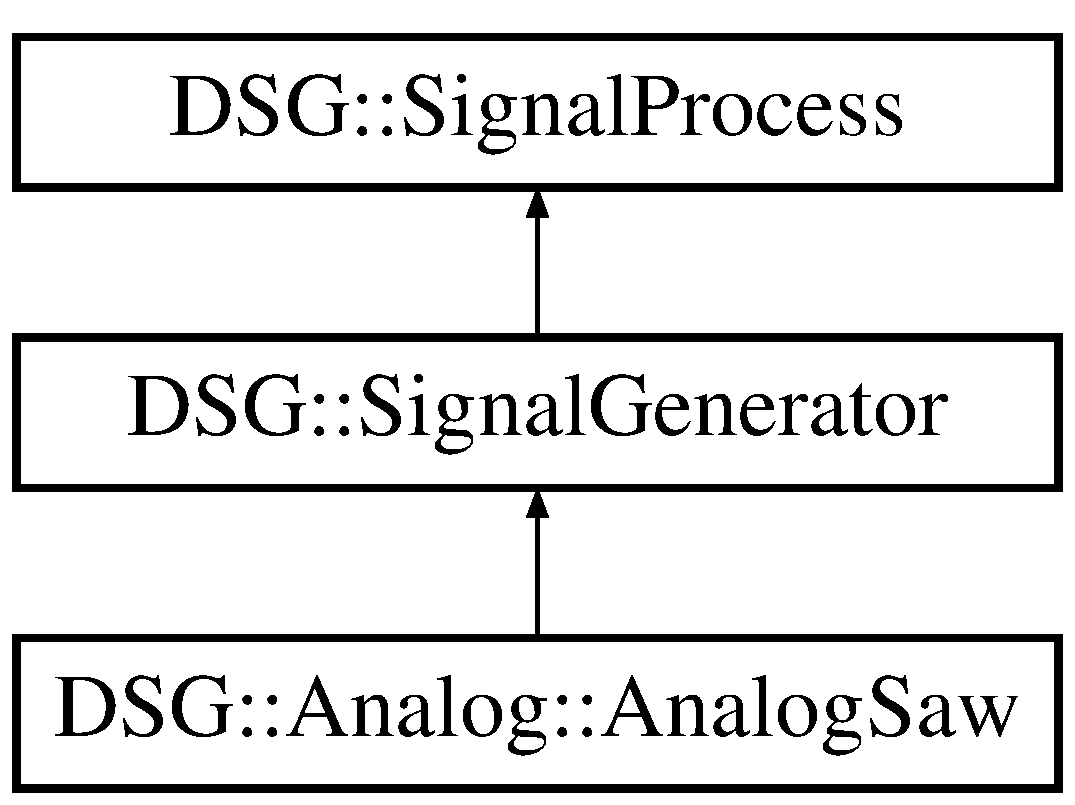
\includegraphics[height=3.000000cm]{class_d_s_g_1_1_analog_1_1_analog_saw}
\end{center}
\end{figure}
\subsection*{Public Member Functions}
\begin{DoxyCompactItemize}
\item 
\hyperlink{class_d_s_g_1_1_analog_1_1_analog_saw_abcb0b997be32413da0d14b93aeeb9c17}{Analog\+Saw} ()
\item 
\hyperlink{class_d_s_g_1_1_analog_1_1_analog_saw_ad110da0b337948fb70ecdfad7dbb5ddf}{Analog\+Saw} (\hyperlink{namespace_d_s_g_a4315a061386fa1014fda09b15d3a6973}{D\+S\+G\+::\+D\+S\+G\+Frequency} const \&frequency, \hyperlink{namespace_d_s_g_a44431ce1eb0a7300efdd207bc879e52c}{D\+S\+G\+::\+D\+S\+G\+Phase} const \&offset)
\item 
virtual \hyperlink{class_d_s_g_1_1_analog_1_1_analog_saw_a42a5fe22e0c3b9d1bd3996fe5bbd24ba}{$\sim$\+Analog\+Saw} ()
\item 
virtual bool \hyperlink{class_d_s_g_1_1_analog_1_1_analog_saw_a8d36e77c09ba84128e786c7bb14cddda}{Perform} (\hyperlink{namespace_d_s_g_ac39a94cd27ebcd9c1e7502d0c624894a}{D\+S\+G\+::\+D\+S\+G\+Sample} \&signal)
\item 
virtual bool \hyperlink{class_d_s_g_1_1_analog_1_1_analog_saw_a38f091059d924c9141fee3e27522e7e1}{Perform} (\hyperlink{class_d_s_g_1_1_ring_buffer}{D\+S\+G\+::\+Ring\+Buffer} \&signal)
\end{DoxyCompactItemize}
\subsection*{Protected Attributes}
\begin{DoxyCompactItemize}
\item 
\hyperlink{namespace_d_s_g_ac39a94cd27ebcd9c1e7502d0c624894a}{D\+S\+G\+::\+D\+S\+G\+Sample} \hyperlink{class_d_s_g_1_1_analog_1_1_analog_saw_a81a923800bb8ba0f788d3567d2965d2a}{\+\_\+stor}
\end{DoxyCompactItemize}
\subsection*{Additional Inherited Members}


\subsection{Detailed Description}
\hyperlink{class_d_s_g_1_1_analog_1_1_analog_saw}{D\+S\+G\+::\+Analog\+::\+Analog\+Saw} -\/ \hyperlink{namespace_d_s_g_1_1_analog}{Analog} Syle Saw Wave Generator. 

Definition at line \hyperlink{_analog_saw_8h_source_l00034}{34} of file \hyperlink{_analog_saw_8h_source}{Analog\+Saw.\+h}.



\subsection{Constructor \& Destructor Documentation}
\hypertarget{class_d_s_g_1_1_analog_1_1_analog_saw_abcb0b997be32413da0d14b93aeeb9c17}{\index{D\+S\+G\+::\+Analog\+::\+Analog\+Saw@{D\+S\+G\+::\+Analog\+::\+Analog\+Saw}!Analog\+Saw@{Analog\+Saw}}
\index{Analog\+Saw@{Analog\+Saw}!D\+S\+G\+::\+Analog\+::\+Analog\+Saw@{D\+S\+G\+::\+Analog\+::\+Analog\+Saw}}
\subsubsection[{Analog\+Saw}]{\setlength{\rightskip}{0pt plus 5cm}D\+S\+G\+::\+Analog\+::\+Analog\+Saw\+::\+Analog\+Saw (
\begin{DoxyParamCaption}
{}
\end{DoxyParamCaption}
)}}\label{class_d_s_g_1_1_analog_1_1_analog_saw_abcb0b997be32413da0d14b93aeeb9c17}


Definition at line \hyperlink{_analog_saw_8cpp_source_l00025}{25} of file \hyperlink{_analog_saw_8cpp_source}{Analog\+Saw.\+cpp}.


\begin{DoxyCode}
00025 :\hyperlink{class_d_s_g_1_1_signal_generator}{DSG::SignalGenerator}()\{\}
\end{DoxyCode}
\hypertarget{class_d_s_g_1_1_analog_1_1_analog_saw_ad110da0b337948fb70ecdfad7dbb5ddf}{\index{D\+S\+G\+::\+Analog\+::\+Analog\+Saw@{D\+S\+G\+::\+Analog\+::\+Analog\+Saw}!Analog\+Saw@{Analog\+Saw}}
\index{Analog\+Saw@{Analog\+Saw}!D\+S\+G\+::\+Analog\+::\+Analog\+Saw@{D\+S\+G\+::\+Analog\+::\+Analog\+Saw}}
\subsubsection[{Analog\+Saw}]{\setlength{\rightskip}{0pt plus 5cm}D\+S\+G\+::\+Analog\+::\+Analog\+Saw\+::\+Analog\+Saw (
\begin{DoxyParamCaption}
\item[{{\bf D\+S\+G\+::\+D\+S\+G\+Frequency} const \&}]{frequency, }
\item[{{\bf D\+S\+G\+::\+D\+S\+G\+Phase} const \&}]{offset}
\end{DoxyParamCaption}
)}}\label{class_d_s_g_1_1_analog_1_1_analog_saw_ad110da0b337948fb70ecdfad7dbb5ddf}


Definition at line \hyperlink{_analog_saw_8cpp_source_l00026}{26} of file \hyperlink{_analog_saw_8cpp_source}{Analog\+Saw.\+cpp}.


\begin{DoxyCode}
00026 :\hyperlink{class_d_s_g_1_1_signal_generator}{DSG::SignalGenerator}(frequency,offset)\{\}
\end{DoxyCode}
\hypertarget{class_d_s_g_1_1_analog_1_1_analog_saw_a42a5fe22e0c3b9d1bd3996fe5bbd24ba}{\index{D\+S\+G\+::\+Analog\+::\+Analog\+Saw@{D\+S\+G\+::\+Analog\+::\+Analog\+Saw}!````~Analog\+Saw@{$\sim$\+Analog\+Saw}}
\index{````~Analog\+Saw@{$\sim$\+Analog\+Saw}!D\+S\+G\+::\+Analog\+::\+Analog\+Saw@{D\+S\+G\+::\+Analog\+::\+Analog\+Saw}}
\subsubsection[{$\sim$\+Analog\+Saw}]{\setlength{\rightskip}{0pt plus 5cm}D\+S\+G\+::\+Analog\+::\+Analog\+Saw\+::$\sim$\+Analog\+Saw (
\begin{DoxyParamCaption}
{}
\end{DoxyParamCaption}
)\hspace{0.3cm}{\ttfamily [virtual]}}}\label{class_d_s_g_1_1_analog_1_1_analog_saw_a42a5fe22e0c3b9d1bd3996fe5bbd24ba}


Definition at line \hyperlink{_analog_saw_8cpp_source_l00027}{27} of file \hyperlink{_analog_saw_8cpp_source}{Analog\+Saw.\+cpp}.


\begin{DoxyCode}
00027 \{\}\end{DoxyCode}


\subsection{Member Function Documentation}
\hypertarget{class_d_s_g_1_1_analog_1_1_analog_saw_a8d36e77c09ba84128e786c7bb14cddda}{\index{D\+S\+G\+::\+Analog\+::\+Analog\+Saw@{D\+S\+G\+::\+Analog\+::\+Analog\+Saw}!Perform@{Perform}}
\index{Perform@{Perform}!D\+S\+G\+::\+Analog\+::\+Analog\+Saw@{D\+S\+G\+::\+Analog\+::\+Analog\+Saw}}
\subsubsection[{Perform}]{\setlength{\rightskip}{0pt plus 5cm}bool D\+S\+G\+::\+Analog\+::\+Analog\+Saw\+::\+Perform (
\begin{DoxyParamCaption}
\item[{{\bf D\+S\+G\+::\+D\+S\+G\+Sample} \&}]{signal}
\end{DoxyParamCaption}
)\hspace{0.3cm}{\ttfamily [inline]}, {\ttfamily [virtual]}}}\label{class_d_s_g_1_1_analog_1_1_analog_saw_a8d36e77c09ba84128e786c7bb14cddda}


Reimplemented from \hyperlink{class_d_s_g_1_1_signal_generator_a46fe75a81a242e191c5049d33ddf4155}{D\+S\+G\+::\+Signal\+Generator}.



Definition at line \hyperlink{_analog_saw_8h_source_l00044}{44} of file \hyperlink{_analog_saw_8h_source}{Analog\+Saw.\+h}.


\begin{DoxyCode}
00044                                                                    \{
00045             \hyperlink{class_d_s_g_1_1_analog_1_1_analog_saw_a81a923800bb8ba0f788d3567d2965d2a}{\_stor}=\hyperlink{class_d_s_g_1_1_phasor_a82c148d71128cfc518fc8e7e131c3a38}{\_phasor};
00046             \hyperlink{class_d_s_g_1_1_analog_1_1_analog_saw_a81a923800bb8ba0f788d3567d2965d2a}{\_stor}+=0.5;
00047             \textcolor{keywordflow}{if} (\hyperlink{class_d_s_g_1_1_analog_1_1_analog_saw_a81a923800bb8ba0f788d3567d2965d2a}{\_stor}>1.0) \{
00048                 --\hyperlink{class_d_s_g_1_1_analog_1_1_analog_saw_a81a923800bb8ba0f788d3567d2965d2a}{\_stor};
00049             \}
00050             \hyperlink{class_d_s_g_1_1_analog_1_1_analog_saw_a81a923800bb8ba0f788d3567d2965d2a}{\_stor}-=0.5;
00051             \hyperlink{class_d_s_g_1_1_analog_1_1_analog_saw_a81a923800bb8ba0f788d3567d2965d2a}{\_stor}*=2.0;
00052             signal=\hyperlink{class_d_s_g_1_1_analog_1_1_analog_saw_a81a923800bb8ba0f788d3567d2965d2a}{\_stor};
00053             \hyperlink{class_d_s_g_1_1_phasor_a6a088b29e506fb5e99d73f4f0160c583}{step}();
00054             \textcolor{keywordflow}{return} \textcolor{keyword}{true};
00055         \}
\end{DoxyCode}
\hypertarget{class_d_s_g_1_1_analog_1_1_analog_saw_a38f091059d924c9141fee3e27522e7e1}{\index{D\+S\+G\+::\+Analog\+::\+Analog\+Saw@{D\+S\+G\+::\+Analog\+::\+Analog\+Saw}!Perform@{Perform}}
\index{Perform@{Perform}!D\+S\+G\+::\+Analog\+::\+Analog\+Saw@{D\+S\+G\+::\+Analog\+::\+Analog\+Saw}}
\subsubsection[{Perform}]{\setlength{\rightskip}{0pt plus 5cm}bool D\+S\+G\+::\+Analog\+::\+Analog\+Saw\+::\+Perform (
\begin{DoxyParamCaption}
\item[{{\bf D\+S\+G\+::\+Ring\+Buffer} \&}]{signal}
\end{DoxyParamCaption}
)\hspace{0.3cm}{\ttfamily [inline]}, {\ttfamily [virtual]}}}\label{class_d_s_g_1_1_analog_1_1_analog_saw_a38f091059d924c9141fee3e27522e7e1}


Reimplemented from \hyperlink{class_d_s_g_1_1_signal_generator_ab050f80e84e6c8b3e354b56930d6a02b}{D\+S\+G\+::\+Signal\+Generator}.



Definition at line \hyperlink{_analog_saw_8h_source_l00056}{56} of file \hyperlink{_analog_saw_8h_source}{Analog\+Saw.\+h}.


\begin{DoxyCode}
00056                                                                     \{
00057             signal.\hyperlink{class_d_s_g_1_1_ring_buffer_ab23c8003d2857809a816068eeb209d60}{Flush}();
00058             \textcolor{keywordflow}{while} (!signal.\hyperlink{class_d_s_g_1_1_ring_buffer_a53ddb04ffcbb5470a8d2b0a3c65b70cb}{Full}()) \{
00059                 \textcolor{keywordflow}{if} (\hyperlink{class_d_s_g_1_1_analog_1_1_analog_saw_a8d36e77c09ba84128e786c7bb14cddda}{Perform}(\hyperlink{class_d_s_g_1_1_signal_generator_a28a9b47a1aa0783029f11a19ba0363f2}{\_storage})) \{
00060                     \textcolor{keywordflow}{if}(signal.\hyperlink{class_d_s_g_1_1_ring_buffer_aa5dd2caa0a270173251faee40a43d692}{Write}(\hyperlink{class_d_s_g_1_1_signal_generator_a28a9b47a1aa0783029f11a19ba0363f2}{\_storage}))\{
00061                     \}\textcolor{keywordflow}{else} \textcolor{keywordflow}{return} \textcolor{keyword}{false};
00062                 \}\textcolor{keywordflow}{else} \textcolor{keywordflow}{return} \textcolor{keyword}{false};
00063             \}\textcolor{keywordflow}{return} \textcolor{keyword}{true};
00064         \}
\end{DoxyCode}


\subsection{Member Data Documentation}
\hypertarget{class_d_s_g_1_1_analog_1_1_analog_saw_a81a923800bb8ba0f788d3567d2965d2a}{\index{D\+S\+G\+::\+Analog\+::\+Analog\+Saw@{D\+S\+G\+::\+Analog\+::\+Analog\+Saw}!\+\_\+stor@{\+\_\+stor}}
\index{\+\_\+stor@{\+\_\+stor}!D\+S\+G\+::\+Analog\+::\+Analog\+Saw@{D\+S\+G\+::\+Analog\+::\+Analog\+Saw}}
\subsubsection[{\+\_\+stor}]{\setlength{\rightskip}{0pt plus 5cm}{\bf D\+S\+G\+::\+D\+S\+G\+Sample} D\+S\+G\+::\+Analog\+::\+Analog\+Saw\+::\+\_\+stor\hspace{0.3cm}{\ttfamily [protected]}}}\label{class_d_s_g_1_1_analog_1_1_analog_saw_a81a923800bb8ba0f788d3567d2965d2a}


Definition at line \hyperlink{_analog_saw_8h_source_l00042}{42} of file \hyperlink{_analog_saw_8h_source}{Analog\+Saw.\+h}.



The documentation for this class was generated from the following files\+:\begin{DoxyCompactItemize}
\item 
\hyperlink{_analog_saw_8h}{Analog\+Saw.\+h}\item 
\hyperlink{_analog_saw_8cpp}{Analog\+Saw.\+cpp}\end{DoxyCompactItemize}

\hypertarget{class_d_s_g_1_1_analog_1_1_analog_square}{\section{D\+S\+G\+:\+:Analog\+:\+:Analog\+Square Class Reference}
\label{class_d_s_g_1_1_analog_1_1_analog_square}\index{D\+S\+G\+::\+Analog\+::\+Analog\+Square@{D\+S\+G\+::\+Analog\+::\+Analog\+Square}}
}


D\+S\+G\+::\+Analog\+Square -\/ \hyperlink{namespace_d_s_g_1_1_analog}{Analog} Syle Square Wave Generator.  




{\ttfamily \#include $<$Analog\+Square.\+h$>$}

Inheritance diagram for D\+S\+G\+:\+:Analog\+:\+:Analog\+Square\+:\begin{figure}[H]
\begin{center}
\leavevmode
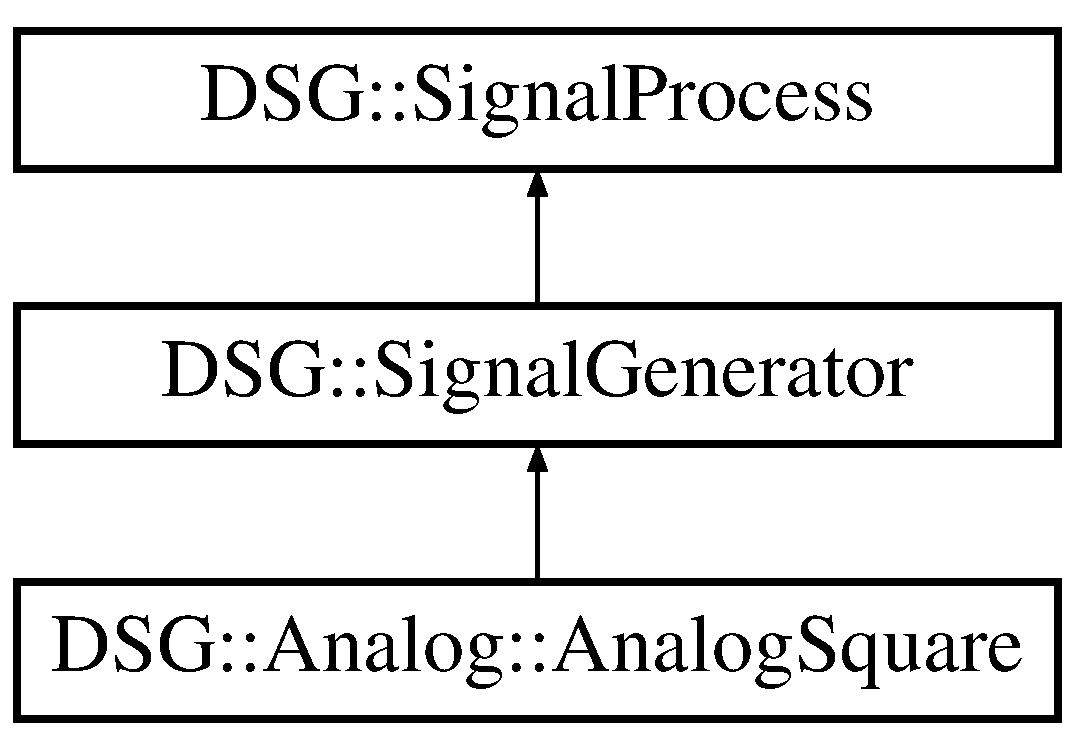
\includegraphics[height=3.000000cm]{class_d_s_g_1_1_analog_1_1_analog_square}
\end{center}
\end{figure}
\subsection*{Public Member Functions}
\begin{DoxyCompactItemize}
\item 
\hypertarget{class_d_s_g_1_1_analog_1_1_analog_square_a886eb67edded43efca895741559a55f4}{{\bfseries Analog\+Square} (D\+S\+G\+::\+D\+S\+G\+Frequency const \&frequency, D\+S\+G\+::\+D\+S\+G\+Phase const \&offset)}\label{class_d_s_g_1_1_analog_1_1_analog_square_a886eb67edded43efca895741559a55f4}

\item 
\hypertarget{class_d_s_g_1_1_analog_1_1_analog_square_a784aa17d266704647789b972cf880e9f}{virtual bool {\bfseries Perform} (D\+S\+G\+::\+D\+S\+G\+Sample \&signal)}\label{class_d_s_g_1_1_analog_1_1_analog_square_a784aa17d266704647789b972cf880e9f}

\item 
\hypertarget{class_d_s_g_1_1_analog_1_1_analog_square_af4d41d5894ae02e920c61e06cf041c60}{virtual bool {\bfseries Perform} (\hyperlink{class_d_s_g_1_1_ring_buffer}{D\+S\+G\+::\+Ring\+Buffer} \&signal)}\label{class_d_s_g_1_1_analog_1_1_analog_square_af4d41d5894ae02e920c61e06cf041c60}

\end{DoxyCompactItemize}
\subsection*{Additional Inherited Members}


\subsection{Detailed Description}
D\+S\+G\+::\+Analog\+Square -\/ \hyperlink{namespace_d_s_g_1_1_analog}{Analog} Syle Square Wave Generator. 

The documentation for this class was generated from the following files\+:\begin{DoxyCompactItemize}
\item 
/\+Users/alexanderzywicki/\+Documents/\+D\+S\+G/src/Analog\+Square.\+h\item 
/\+Users/alexanderzywicki/\+Documents/\+D\+S\+G/src/Analog\+Square.\+cpp\end{DoxyCompactItemize}

\hypertarget{class_d_s_g_1_1_analog_1_1_analog_triangle}{\section{D\+S\+G\+:\+:Analog\+:\+:Analog\+Triangle Class Reference}
\label{class_d_s_g_1_1_analog_1_1_analog_triangle}\index{D\+S\+G\+::\+Analog\+::\+Analog\+Triangle@{D\+S\+G\+::\+Analog\+::\+Analog\+Triangle}}
}


\hyperlink{class_d_s_g_1_1_analog_1_1_analog_triangle}{D\+S\+G\+::\+Analog\+::\+Analog\+Triangle} -\/ \hyperlink{namespace_d_s_g_1_1_analog}{Analog} Syle Triangle Wave Generator.  




{\ttfamily \#include $<$Analog\+Triangle.\+h$>$}

Inheritance diagram for D\+S\+G\+:\+:Analog\+:\+:Analog\+Triangle\+:\begin{figure}[H]
\begin{center}
\leavevmode
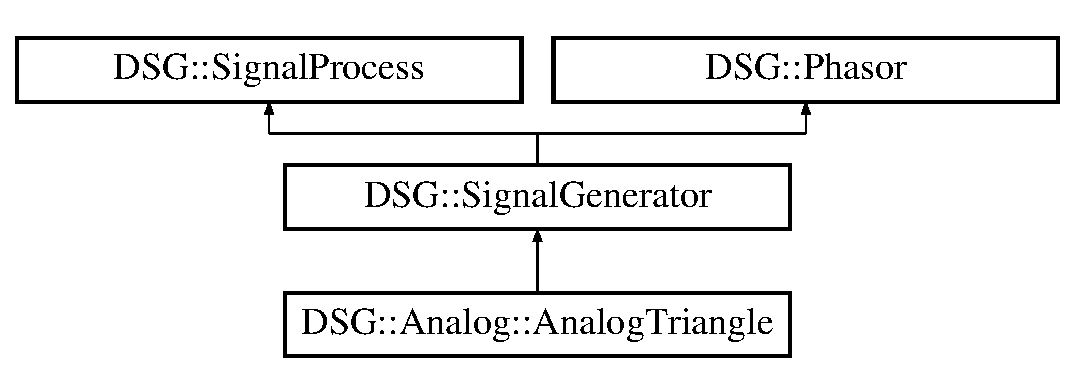
\includegraphics[height=3.000000cm]{class_d_s_g_1_1_analog_1_1_analog_triangle}
\end{center}
\end{figure}
\subsection*{Public Member Functions}
\begin{DoxyCompactItemize}
\item 
\hyperlink{class_d_s_g_1_1_analog_1_1_analog_triangle_a2fe1a7a29eb9472323a2a1c0d0696e55}{Analog\+Triangle} ()
\item 
\hyperlink{class_d_s_g_1_1_analog_1_1_analog_triangle_a75c0a8b20e1843b35de3944da11c75ed}{Analog\+Triangle} (\hyperlink{namespace_d_s_g_a4315a061386fa1014fda09b15d3a6973}{D\+S\+G\+::\+D\+S\+G\+Frequency} const \&frequency, \hyperlink{namespace_d_s_g_a44431ce1eb0a7300efdd207bc879e52c}{D\+S\+G\+::\+D\+S\+G\+Phase} const \&offset)
\item 
virtual \hyperlink{class_d_s_g_1_1_analog_1_1_analog_triangle_af6e127d2fb623afad9b172e7c8b3c656}{$\sim$\+Analog\+Triangle} ()
\item 
virtual bool \hyperlink{class_d_s_g_1_1_analog_1_1_analog_triangle_a9b2484f3eb4c4ad545cb88b8833be124}{Perform} (\hyperlink{namespace_d_s_g_ac39a94cd27ebcd9c1e7502d0c624894a}{D\+S\+G\+::\+D\+S\+G\+Sample} \&signal)
\item 
virtual bool \hyperlink{class_d_s_g_1_1_analog_1_1_analog_triangle_a568c994e0f83f6a01d813357259a8f37}{Perform} (\hyperlink{class_d_s_g_1_1_ring_buffer}{D\+S\+G\+::\+Ring\+Buffer} \&signal)
\end{DoxyCompactItemize}
\subsection*{Protected Attributes}
\begin{DoxyCompactItemize}
\item 
\hyperlink{namespace_d_s_g_ac39a94cd27ebcd9c1e7502d0c624894a}{D\+S\+G\+::\+D\+S\+G\+Sample} \hyperlink{class_d_s_g_1_1_analog_1_1_analog_triangle_ac93bccb7e366491f45ea9c3af04072ae}{\+\_\+stor}
\end{DoxyCompactItemize}
\subsection*{Additional Inherited Members}


\subsection{Detailed Description}
\hyperlink{class_d_s_g_1_1_analog_1_1_analog_triangle}{D\+S\+G\+::\+Analog\+::\+Analog\+Triangle} -\/ \hyperlink{namespace_d_s_g_1_1_analog}{Analog} Syle Triangle Wave Generator. 

Definition at line \hyperlink{_analog_triangle_8h_source_l00034}{34} of file \hyperlink{_analog_triangle_8h_source}{Analog\+Triangle.\+h}.



\subsection{Constructor \& Destructor Documentation}
\hypertarget{class_d_s_g_1_1_analog_1_1_analog_triangle_a2fe1a7a29eb9472323a2a1c0d0696e55}{\index{D\+S\+G\+::\+Analog\+::\+Analog\+Triangle@{D\+S\+G\+::\+Analog\+::\+Analog\+Triangle}!Analog\+Triangle@{Analog\+Triangle}}
\index{Analog\+Triangle@{Analog\+Triangle}!D\+S\+G\+::\+Analog\+::\+Analog\+Triangle@{D\+S\+G\+::\+Analog\+::\+Analog\+Triangle}}
\subsubsection[{Analog\+Triangle}]{\setlength{\rightskip}{0pt plus 5cm}D\+S\+G\+::\+Analog\+::\+Analog\+Triangle\+::\+Analog\+Triangle (
\begin{DoxyParamCaption}
{}
\end{DoxyParamCaption}
)}}\label{class_d_s_g_1_1_analog_1_1_analog_triangle_a2fe1a7a29eb9472323a2a1c0d0696e55}


Definition at line \hyperlink{_analog_triangle_8cpp_source_l00025}{25} of file \hyperlink{_analog_triangle_8cpp_source}{Analog\+Triangle.\+cpp}.


\begin{DoxyCode}
00025 :\hyperlink{class_d_s_g_1_1_signal_generator}{DSG::SignalGenerator}()\{\}
\end{DoxyCode}
\hypertarget{class_d_s_g_1_1_analog_1_1_analog_triangle_a75c0a8b20e1843b35de3944da11c75ed}{\index{D\+S\+G\+::\+Analog\+::\+Analog\+Triangle@{D\+S\+G\+::\+Analog\+::\+Analog\+Triangle}!Analog\+Triangle@{Analog\+Triangle}}
\index{Analog\+Triangle@{Analog\+Triangle}!D\+S\+G\+::\+Analog\+::\+Analog\+Triangle@{D\+S\+G\+::\+Analog\+::\+Analog\+Triangle}}
\subsubsection[{Analog\+Triangle}]{\setlength{\rightskip}{0pt plus 5cm}D\+S\+G\+::\+Analog\+::\+Analog\+Triangle\+::\+Analog\+Triangle (
\begin{DoxyParamCaption}
\item[{{\bf D\+S\+G\+::\+D\+S\+G\+Frequency} const \&}]{frequency, }
\item[{{\bf D\+S\+G\+::\+D\+S\+G\+Phase} const \&}]{offset}
\end{DoxyParamCaption}
)}}\label{class_d_s_g_1_1_analog_1_1_analog_triangle_a75c0a8b20e1843b35de3944da11c75ed}


Definition at line \hyperlink{_analog_triangle_8cpp_source_l00026}{26} of file \hyperlink{_analog_triangle_8cpp_source}{Analog\+Triangle.\+cpp}.


\begin{DoxyCode}
00026 :\hyperlink{class_d_s_g_1_1_signal_generator}{DSG::SignalGenerator}(frequency,offset)\{\}
\end{DoxyCode}
\hypertarget{class_d_s_g_1_1_analog_1_1_analog_triangle_af6e127d2fb623afad9b172e7c8b3c656}{\index{D\+S\+G\+::\+Analog\+::\+Analog\+Triangle@{D\+S\+G\+::\+Analog\+::\+Analog\+Triangle}!````~Analog\+Triangle@{$\sim$\+Analog\+Triangle}}
\index{````~Analog\+Triangle@{$\sim$\+Analog\+Triangle}!D\+S\+G\+::\+Analog\+::\+Analog\+Triangle@{D\+S\+G\+::\+Analog\+::\+Analog\+Triangle}}
\subsubsection[{$\sim$\+Analog\+Triangle}]{\setlength{\rightskip}{0pt plus 5cm}D\+S\+G\+::\+Analog\+::\+Analog\+Triangle\+::$\sim$\+Analog\+Triangle (
\begin{DoxyParamCaption}
{}
\end{DoxyParamCaption}
)\hspace{0.3cm}{\ttfamily [virtual]}}}\label{class_d_s_g_1_1_analog_1_1_analog_triangle_af6e127d2fb623afad9b172e7c8b3c656}


Definition at line \hyperlink{_analog_triangle_8cpp_source_l00027}{27} of file \hyperlink{_analog_triangle_8cpp_source}{Analog\+Triangle.\+cpp}.


\begin{DoxyCode}
00027 \{\}\end{DoxyCode}


\subsection{Member Function Documentation}
\hypertarget{class_d_s_g_1_1_analog_1_1_analog_triangle_a9b2484f3eb4c4ad545cb88b8833be124}{\index{D\+S\+G\+::\+Analog\+::\+Analog\+Triangle@{D\+S\+G\+::\+Analog\+::\+Analog\+Triangle}!Perform@{Perform}}
\index{Perform@{Perform}!D\+S\+G\+::\+Analog\+::\+Analog\+Triangle@{D\+S\+G\+::\+Analog\+::\+Analog\+Triangle}}
\subsubsection[{Perform}]{\setlength{\rightskip}{0pt plus 5cm}bool D\+S\+G\+::\+Analog\+::\+Analog\+Triangle\+::\+Perform (
\begin{DoxyParamCaption}
\item[{{\bf D\+S\+G\+::\+D\+S\+G\+Sample} \&}]{signal}
\end{DoxyParamCaption}
)\hspace{0.3cm}{\ttfamily [inline]}, {\ttfamily [virtual]}}}\label{class_d_s_g_1_1_analog_1_1_analog_triangle_a9b2484f3eb4c4ad545cb88b8833be124}


Reimplemented from \hyperlink{class_d_s_g_1_1_signal_generator_a46fe75a81a242e191c5049d33ddf4155}{D\+S\+G\+::\+Signal\+Generator}.



Definition at line \hyperlink{_analog_triangle_8h_source_l00044}{44} of file \hyperlink{_analog_triangle_8h_source}{Analog\+Triangle.\+h}.


\begin{DoxyCode}
00044                                                                         \{
00045             \hyperlink{class_d_s_g_1_1_analog_1_1_analog_triangle_ac93bccb7e366491f45ea9c3af04072ae}{\_stor} = \hyperlink{class_d_s_g_1_1_phasor_a82c148d71128cfc518fc8e7e131c3a38}{\_phasor};
00046             \hyperlink{class_d_s_g_1_1_analog_1_1_analog_triangle_ac93bccb7e366491f45ea9c3af04072ae}{\_stor}+=0.25;
00047             \textcolor{keywordflow}{while} (\hyperlink{class_d_s_g_1_1_analog_1_1_analog_triangle_ac93bccb7e366491f45ea9c3af04072ae}{\_stor}>1.0) \{
00048                 \hyperlink{class_d_s_g_1_1_analog_1_1_analog_triangle_ac93bccb7e366491f45ea9c3af04072ae}{\_stor}-=1.0;
00049             \}
00050             \hyperlink{class_d_s_g_1_1_analog_1_1_analog_triangle_ac93bccb7e366491f45ea9c3af04072ae}{\_stor}-=0.5;
00051             \textcolor{keywordflow}{if} (\hyperlink{class_d_s_g_1_1_analog_1_1_analog_triangle_ac93bccb7e366491f45ea9c3af04072ae}{\_stor}<0) \{
00052                 \hyperlink{class_d_s_g_1_1_analog_1_1_analog_triangle_ac93bccb7e366491f45ea9c3af04072ae}{\_stor}*=-1.0;
00053             \}
00054             \hyperlink{class_d_s_g_1_1_analog_1_1_analog_triangle_ac93bccb7e366491f45ea9c3af04072ae}{\_stor}-=0.25;
00055             \hyperlink{class_d_s_g_1_1_analog_1_1_analog_triangle_ac93bccb7e366491f45ea9c3af04072ae}{\_stor}*=-4.0;
00056             signal = \hyperlink{class_d_s_g_1_1_analog_1_1_analog_triangle_ac93bccb7e366491f45ea9c3af04072ae}{\_stor};
00057             \hyperlink{class_d_s_g_1_1_phasor_a6a088b29e506fb5e99d73f4f0160c583}{step}();\textcolor{comment}{//always last}
00058             \textcolor{keywordflow}{return} \textcolor{keyword}{true};
00059         \}
\end{DoxyCode}
\hypertarget{class_d_s_g_1_1_analog_1_1_analog_triangle_a568c994e0f83f6a01d813357259a8f37}{\index{D\+S\+G\+::\+Analog\+::\+Analog\+Triangle@{D\+S\+G\+::\+Analog\+::\+Analog\+Triangle}!Perform@{Perform}}
\index{Perform@{Perform}!D\+S\+G\+::\+Analog\+::\+Analog\+Triangle@{D\+S\+G\+::\+Analog\+::\+Analog\+Triangle}}
\subsubsection[{Perform}]{\setlength{\rightskip}{0pt plus 5cm}bool D\+S\+G\+::\+Analog\+::\+Analog\+Triangle\+::\+Perform (
\begin{DoxyParamCaption}
\item[{{\bf D\+S\+G\+::\+Ring\+Buffer} \&}]{signal}
\end{DoxyParamCaption}
)\hspace{0.3cm}{\ttfamily [inline]}, {\ttfamily [virtual]}}}\label{class_d_s_g_1_1_analog_1_1_analog_triangle_a568c994e0f83f6a01d813357259a8f37}


Reimplemented from \hyperlink{class_d_s_g_1_1_signal_generator_ab050f80e84e6c8b3e354b56930d6a02b}{D\+S\+G\+::\+Signal\+Generator}.



Definition at line \hyperlink{_analog_triangle_8h_source_l00060}{60} of file \hyperlink{_analog_triangle_8h_source}{Analog\+Triangle.\+h}.


\begin{DoxyCode}
00060                                                                          \{
00061             signal.\hyperlink{class_d_s_g_1_1_ring_buffer_ab23c8003d2857809a816068eeb209d60}{Flush}();
00062             \textcolor{keywordflow}{while} (!signal.\hyperlink{class_d_s_g_1_1_ring_buffer_a53ddb04ffcbb5470a8d2b0a3c65b70cb}{Full}()) \{
00063                 \textcolor{keywordflow}{if} (\hyperlink{class_d_s_g_1_1_analog_1_1_analog_triangle_a9b2484f3eb4c4ad545cb88b8833be124}{Perform}(\hyperlink{class_d_s_g_1_1_signal_generator_a28a9b47a1aa0783029f11a19ba0363f2}{\_storage})) \{
00064                     \textcolor{keywordflow}{if}(signal.\hyperlink{class_d_s_g_1_1_ring_buffer_aa5dd2caa0a270173251faee40a43d692}{Write}(\hyperlink{class_d_s_g_1_1_signal_generator_a28a9b47a1aa0783029f11a19ba0363f2}{\_storage}))\{
00065                     \}\textcolor{keywordflow}{else} \textcolor{keywordflow}{return} \textcolor{keyword}{false};
00066                 \}\textcolor{keywordflow}{else} \textcolor{keywordflow}{return} \textcolor{keyword}{false};
00067             \}\textcolor{keywordflow}{return} \textcolor{keyword}{true};
00068         \}
\end{DoxyCode}


\subsection{Member Data Documentation}
\hypertarget{class_d_s_g_1_1_analog_1_1_analog_triangle_ac93bccb7e366491f45ea9c3af04072ae}{\index{D\+S\+G\+::\+Analog\+::\+Analog\+Triangle@{D\+S\+G\+::\+Analog\+::\+Analog\+Triangle}!\+\_\+stor@{\+\_\+stor}}
\index{\+\_\+stor@{\+\_\+stor}!D\+S\+G\+::\+Analog\+::\+Analog\+Triangle@{D\+S\+G\+::\+Analog\+::\+Analog\+Triangle}}
\subsubsection[{\+\_\+stor}]{\setlength{\rightskip}{0pt plus 5cm}{\bf D\+S\+G\+::\+D\+S\+G\+Sample} D\+S\+G\+::\+Analog\+::\+Analog\+Triangle\+::\+\_\+stor\hspace{0.3cm}{\ttfamily [protected]}}}\label{class_d_s_g_1_1_analog_1_1_analog_triangle_ac93bccb7e366491f45ea9c3af04072ae}


Definition at line \hyperlink{_analog_triangle_8h_source_l00042}{42} of file \hyperlink{_analog_triangle_8h_source}{Analog\+Triangle.\+h}.



The documentation for this class was generated from the following files\+:\begin{DoxyCompactItemize}
\item 
\hyperlink{_analog_triangle_8h}{Analog\+Triangle.\+h}\item 
\hyperlink{_analog_triangle_8cpp}{Analog\+Triangle.\+cpp}\end{DoxyCompactItemize}

\hypertarget{class_d_s_g_1_1_audio_settings}{\section{D\+S\+G\+:\+:Audio\+Settings Class Reference}
\label{class_d_s_g_1_1_audio_settings}\index{D\+S\+G\+::\+Audio\+Settings@{D\+S\+G\+::\+Audio\+Settings}}
}


\hyperlink{class_d_s_g_1_1_audio_settings}{D\+S\+G\+::\+Audio\+Settings} -\/ Global Storage For Audio Settings Such As Sample Rate.  




{\ttfamily \#include $<$Audio\+Settings.\+h$>$}

\subsection*{Static Public Member Functions}
\begin{DoxyCompactItemize}
\item 
static \hyperlink{namespace_d_s_g_a4315a061386fa1014fda09b15d3a6973}{D\+S\+G\+::\+D\+S\+G\+Frequency} const \& \hyperlink{class_d_s_g_1_1_audio_settings_a4f459c389b10c11828e2f2f00c012c49}{Sample\+Rate} ()
\item 
static \hyperlink{namespace_d_s_g_a4315a061386fa1014fda09b15d3a6973}{D\+S\+G\+::\+D\+S\+G\+Frequency} const \& \hyperlink{class_d_s_g_1_1_audio_settings_a9c5640e47b6eaa4331a0e5053abb1314}{Sample\+Rate} (\hyperlink{namespace_d_s_g_a4315a061386fa1014fda09b15d3a6973}{D\+S\+G\+::\+D\+S\+G\+Frequency} const \&value)
\item 
static \hyperlink{namespace_d_s_g_a4315a061386fa1014fda09b15d3a6973}{D\+S\+G\+::\+D\+S\+G\+Frequency} const \& \hyperlink{class_d_s_g_1_1_audio_settings_a8cb4afd7b58e927300ff46fbeb71bec7}{Nyquist} ()
\end{DoxyCompactItemize}
\subsection*{Static Protected Attributes}
\begin{DoxyCompactItemize}
\item 
static \hyperlink{namespace_d_s_g_a4315a061386fa1014fda09b15d3a6973}{D\+S\+G\+::\+D\+S\+G\+Frequency} \hyperlink{class_d_s_g_1_1_audio_settings_a56869b51933f102b197f54001c8a1d27}{\+\_\+sample\+Rate}
\item 
static \hyperlink{namespace_d_s_g_a4315a061386fa1014fda09b15d3a6973}{D\+S\+G\+::\+D\+S\+G\+Frequency} \hyperlink{class_d_s_g_1_1_audio_settings_af3c7cbd15390d9bcbe39983c069390b5}{\+\_\+nyquist}
\end{DoxyCompactItemize}


\subsection{Detailed Description}
\hyperlink{class_d_s_g_1_1_audio_settings}{D\+S\+G\+::\+Audio\+Settings} -\/ Global Storage For Audio Settings Such As Sample Rate. 

Definition at line \hyperlink{_audio_settings_8h_source_l00014}{14} of file \hyperlink{_audio_settings_8h_source}{Audio\+Settings.\+h}.



\subsection{Member Function Documentation}
\hypertarget{class_d_s_g_1_1_audio_settings_a8cb4afd7b58e927300ff46fbeb71bec7}{\index{D\+S\+G\+::\+Audio\+Settings@{D\+S\+G\+::\+Audio\+Settings}!Nyquist@{Nyquist}}
\index{Nyquist@{Nyquist}!D\+S\+G\+::\+Audio\+Settings@{D\+S\+G\+::\+Audio\+Settings}}
\subsubsection[{Nyquist}]{\setlength{\rightskip}{0pt plus 5cm}{\bf D\+S\+G\+::\+D\+S\+G\+Frequency} const \& D\+S\+G\+::\+Audio\+Settings\+::\+Nyquist (
\begin{DoxyParamCaption}
{}
\end{DoxyParamCaption}
)\hspace{0.3cm}{\ttfamily [static]}}}\label{class_d_s_g_1_1_audio_settings_a8cb4afd7b58e927300ff46fbeb71bec7}


Definition at line \hyperlink{_audio_settings_8cpp_source_l00019}{19} of file \hyperlink{_audio_settings_8cpp_source}{Audio\+Settings.\+cpp}.


\begin{DoxyCode}
00019                                                 \{
00020     \textcolor{keywordflow}{return} \hyperlink{class_d_s_g_1_1_audio_settings_af3c7cbd15390d9bcbe39983c069390b5}{\_nyquist};
00021 \}\end{DoxyCode}
\hypertarget{class_d_s_g_1_1_audio_settings_a4f459c389b10c11828e2f2f00c012c49}{\index{D\+S\+G\+::\+Audio\+Settings@{D\+S\+G\+::\+Audio\+Settings}!Sample\+Rate@{Sample\+Rate}}
\index{Sample\+Rate@{Sample\+Rate}!D\+S\+G\+::\+Audio\+Settings@{D\+S\+G\+::\+Audio\+Settings}}
\subsubsection[{Sample\+Rate}]{\setlength{\rightskip}{0pt plus 5cm}{\bf D\+S\+G\+::\+D\+S\+G\+Frequency} const \& D\+S\+G\+::\+Audio\+Settings\+::\+Sample\+Rate (
\begin{DoxyParamCaption}
{}
\end{DoxyParamCaption}
)\hspace{0.3cm}{\ttfamily [static]}}}\label{class_d_s_g_1_1_audio_settings_a4f459c389b10c11828e2f2f00c012c49}


Definition at line \hyperlink{_audio_settings_8cpp_source_l00011}{11} of file \hyperlink{_audio_settings_8cpp_source}{Audio\+Settings.\+cpp}.


\begin{DoxyCode}
00011                                                    \{
00012     \textcolor{keywordflow}{return} \hyperlink{class_d_s_g_1_1_audio_settings_a56869b51933f102b197f54001c8a1d27}{\_sampleRate};
00013 \}
\end{DoxyCode}
\hypertarget{class_d_s_g_1_1_audio_settings_a9c5640e47b6eaa4331a0e5053abb1314}{\index{D\+S\+G\+::\+Audio\+Settings@{D\+S\+G\+::\+Audio\+Settings}!Sample\+Rate@{Sample\+Rate}}
\index{Sample\+Rate@{Sample\+Rate}!D\+S\+G\+::\+Audio\+Settings@{D\+S\+G\+::\+Audio\+Settings}}
\subsubsection[{Sample\+Rate}]{\setlength{\rightskip}{0pt plus 5cm}{\bf D\+S\+G\+::\+D\+S\+G\+Frequency} const \& D\+S\+G\+::\+Audio\+Settings\+::\+Sample\+Rate (
\begin{DoxyParamCaption}
\item[{{\bf D\+S\+G\+::\+D\+S\+G\+Frequency} const \&}]{value}
\end{DoxyParamCaption}
)\hspace{0.3cm}{\ttfamily [static]}}}\label{class_d_s_g_1_1_audio_settings_a9c5640e47b6eaa4331a0e5053abb1314}


Definition at line \hyperlink{_audio_settings_8cpp_source_l00014}{14} of file \hyperlink{_audio_settings_8cpp_source}{Audio\+Settings.\+cpp}.


\begin{DoxyCode}
00014                                                                                \{
00015     \hyperlink{class_d_s_g_1_1_audio_settings_a56869b51933f102b197f54001c8a1d27}{\_sampleRate} = value;
00016     \hyperlink{class_d_s_g_1_1_audio_settings_af3c7cbd15390d9bcbe39983c069390b5}{\_nyquist} = \hyperlink{class_d_s_g_1_1_audio_settings_a56869b51933f102b197f54001c8a1d27}{\_sampleRate}*0.5;
00017     \textcolor{keywordflow}{return} \hyperlink{class_d_s_g_1_1_audio_settings_a56869b51933f102b197f54001c8a1d27}{\_sampleRate};
00018 \}
\end{DoxyCode}


\subsection{Member Data Documentation}
\hypertarget{class_d_s_g_1_1_audio_settings_af3c7cbd15390d9bcbe39983c069390b5}{\index{D\+S\+G\+::\+Audio\+Settings@{D\+S\+G\+::\+Audio\+Settings}!\+\_\+nyquist@{\+\_\+nyquist}}
\index{\+\_\+nyquist@{\+\_\+nyquist}!D\+S\+G\+::\+Audio\+Settings@{D\+S\+G\+::\+Audio\+Settings}}
\subsubsection[{\+\_\+nyquist}]{\setlength{\rightskip}{0pt plus 5cm}{\bf D\+S\+G\+::\+D\+S\+G\+Frequency} D\+S\+G\+::\+Audio\+Settings\+::\+\_\+nyquist\hspace{0.3cm}{\ttfamily [static]}, {\ttfamily [protected]}}}\label{class_d_s_g_1_1_audio_settings_af3c7cbd15390d9bcbe39983c069390b5}


Definition at line \hyperlink{_audio_settings_8h_source_l00021}{21} of file \hyperlink{_audio_settings_8h_source}{Audio\+Settings.\+h}.

\hypertarget{class_d_s_g_1_1_audio_settings_a56869b51933f102b197f54001c8a1d27}{\index{D\+S\+G\+::\+Audio\+Settings@{D\+S\+G\+::\+Audio\+Settings}!\+\_\+sample\+Rate@{\+\_\+sample\+Rate}}
\index{\+\_\+sample\+Rate@{\+\_\+sample\+Rate}!D\+S\+G\+::\+Audio\+Settings@{D\+S\+G\+::\+Audio\+Settings}}
\subsubsection[{\+\_\+sample\+Rate}]{\setlength{\rightskip}{0pt plus 5cm}{\bf D\+S\+G\+::\+D\+S\+G\+Frequency} D\+S\+G\+::\+Audio\+Settings\+::\+\_\+sample\+Rate\hspace{0.3cm}{\ttfamily [static]}, {\ttfamily [protected]}}}\label{class_d_s_g_1_1_audio_settings_a56869b51933f102b197f54001c8a1d27}


Definition at line \hyperlink{_audio_settings_8h_source_l00020}{20} of file \hyperlink{_audio_settings_8h_source}{Audio\+Settings.\+h}.



The documentation for this class was generated from the following files\+:\begin{DoxyCompactItemize}
\item 
/\+Users/alexanderzywicki/\+Documents/\+D\+S\+G/src/\hyperlink{_audio_settings_8h}{Audio\+Settings.\+h}\item 
/\+Users/alexanderzywicki/\+Documents/\+D\+S\+G/src/\hyperlink{_audio_settings_8cpp}{Audio\+Settings.\+cpp}\end{DoxyCompactItemize}

\hypertarget{class_d_s_g_1_1_b_l_i_t_1_1_blit}{\section{D\+S\+G\+:\+:B\+L\+I\+T\+:\+:Blit Class Reference}
\label{class_d_s_g_1_1_b_l_i_t_1_1_blit}\index{D\+S\+G\+::\+B\+L\+I\+T\+::\+Blit@{D\+S\+G\+::\+B\+L\+I\+T\+::\+Blit}}
}


\hyperlink{class_d_s_g_1_1_b_l_i_t_1_1_blit}{D\+S\+G\+::\+B\+L\+I\+T\+::\+Blit} -\/ Band-\/\+Limited Impulse Train Generator.  




{\ttfamily \#include $<$B\+L\+I\+T.\+h$>$}

Inheritance diagram for D\+S\+G\+:\+:B\+L\+I\+T\+:\+:Blit\+:\begin{figure}[H]
\begin{center}
\leavevmode
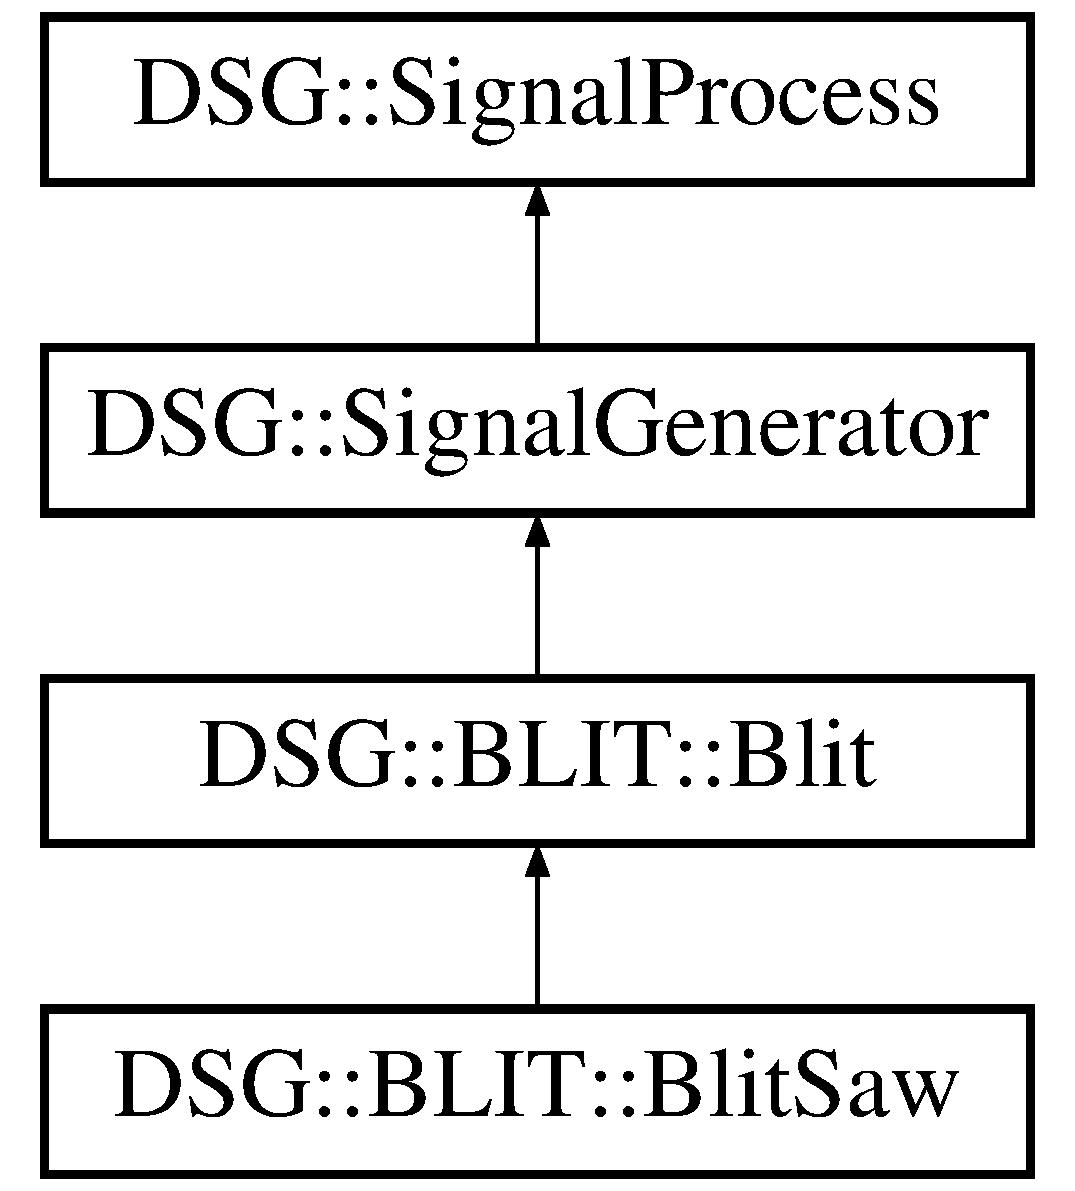
\includegraphics[height=4.000000cm]{class_d_s_g_1_1_b_l_i_t_1_1_blit}
\end{center}
\end{figure}
\subsection*{Public Member Functions}
\begin{DoxyCompactItemize}
\item 
\hyperlink{class_d_s_g_1_1_b_l_i_t_1_1_blit_a1d9bed6285a8b3c0e073f3e3662716af}{Blit} ()
\item 
\hyperlink{class_d_s_g_1_1_b_l_i_t_1_1_blit_a8ab0fb1b908d641527bb86a81d1722ba}{Blit} (\hyperlink{namespace_d_s_g_a4315a061386fa1014fda09b15d3a6973}{D\+S\+G\+::\+D\+S\+G\+Frequency} const \&frequency, \hyperlink{namespace_d_s_g_a44431ce1eb0a7300efdd207bc879e52c}{D\+S\+G\+::\+D\+S\+G\+Phase} const \&offset)
\item 
virtual \hyperlink{class_d_s_g_1_1_b_l_i_t_1_1_blit_a92da2e1763735b3e17f7b9a24377f988}{$\sim$\+Blit} ()
\item 
virtual bool \hyperlink{class_d_s_g_1_1_b_l_i_t_1_1_blit_adfd7c8891b4c4dbd0530a2780781b2bd}{Perform} (\hyperlink{namespace_d_s_g_ac39a94cd27ebcd9c1e7502d0c624894a}{D\+S\+G\+::\+D\+S\+G\+Sample} \&signal)
\item 
virtual bool \hyperlink{class_d_s_g_1_1_b_l_i_t_1_1_blit_aab7c67ff8f059c8367ba316cf8cd5436}{Perform} (\hyperlink{class_d_s_g_1_1_ring_buffer}{D\+S\+G\+::\+Ring\+Buffer} \&signal)
\item 
virtual \hyperlink{namespace_d_s_g_a4315a061386fa1014fda09b15d3a6973}{D\+S\+G\+::\+D\+S\+G\+Frequency} const \& \hyperlink{class_d_s_g_1_1_b_l_i_t_1_1_blit_a933f8f9f324a4fde4f9e2b69473d88ed}{Frequency} (\hyperlink{namespace_d_s_g_a4315a061386fa1014fda09b15d3a6973}{D\+S\+G\+::\+D\+S\+G\+Frequency} const \&\hyperlink{class_d_s_g_1_1_b_l_i_t_1_1_blit_ac8fb9d4fb45d0697bf364bb5d6b570ce}{value})
\end{DoxyCompactItemize}
\subsection*{Protected Attributes}
\begin{DoxyCompactItemize}
\item 
unsigned long \hyperlink{class_d_s_g_1_1_b_l_i_t_1_1_blit_a04d7d6b22a386428e5c25668e1587794}{p\+\_\+}
\item 
unsigned long \hyperlink{class_d_s_g_1_1_b_l_i_t_1_1_blit_afa6e4d46efdbfa032762610601ed42a0}{m\+\_\+}
\item 
unsigned long \hyperlink{class_d_s_g_1_1_b_l_i_t_1_1_blit_a632c6f070187969b90c70b65668b82bc}{\+\_\+h}
\item 
double \hyperlink{class_d_s_g_1_1_b_l_i_t_1_1_blit_a66e2a97840ad0772daaaa9aea63b77b4}{a\+\_\+}
\item 
\hyperlink{namespace_d_s_g_ac39a94cd27ebcd9c1e7502d0c624894a}{D\+S\+G\+::\+D\+S\+G\+Sample} \hyperlink{class_d_s_g_1_1_b_l_i_t_1_1_blit_a6de89a5a240f226c940aef97661c9cee}{denominator}
\item 
\hyperlink{namespace_d_s_g_ac39a94cd27ebcd9c1e7502d0c624894a}{D\+S\+G\+::\+D\+S\+G\+Sample} \hyperlink{class_d_s_g_1_1_b_l_i_t_1_1_blit_ac8fb9d4fb45d0697bf364bb5d6b570ce}{value}
\end{DoxyCompactItemize}
\subsection*{Additional Inherited Members}


\subsection{Detailed Description}
\hyperlink{class_d_s_g_1_1_b_l_i_t_1_1_blit}{D\+S\+G\+::\+B\+L\+I\+T\+::\+Blit} -\/ Band-\/\+Limited Impulse Train Generator. 

\begin{DoxyRefDesc}{Todo}
\item[\hyperlink{todo__todo000001}{Todo}]Re-\/write \hyperlink{class_d_s_g_1_1_b_l_i_t_1_1_blit}{D\+S\+G\+::\+B\+L\+I\+T\+::\+Blit} algorithm \end{DoxyRefDesc}


Definition at line \hyperlink{_b_l_i_t_8h_source_l00039}{39} of file \hyperlink{_b_l_i_t_8h_source}{B\+L\+I\+T.\+h}.



\subsection{Constructor \& Destructor Documentation}
\hypertarget{class_d_s_g_1_1_b_l_i_t_1_1_blit_a1d9bed6285a8b3c0e073f3e3662716af}{\index{D\+S\+G\+::\+B\+L\+I\+T\+::\+Blit@{D\+S\+G\+::\+B\+L\+I\+T\+::\+Blit}!Blit@{Blit}}
\index{Blit@{Blit}!D\+S\+G\+::\+B\+L\+I\+T\+::\+Blit@{D\+S\+G\+::\+B\+L\+I\+T\+::\+Blit}}
\subsubsection[{Blit}]{\setlength{\rightskip}{0pt plus 5cm}D\+S\+G\+::\+B\+L\+I\+T\+::\+Blit\+::\+Blit (
\begin{DoxyParamCaption}
{}
\end{DoxyParamCaption}
)}}\label{class_d_s_g_1_1_b_l_i_t_1_1_blit_a1d9bed6285a8b3c0e073f3e3662716af}


Definition at line \hyperlink{_b_l_i_t_8cpp_source_l00025}{25} of file \hyperlink{_b_l_i_t_8cpp_source}{B\+L\+I\+T.\+cpp}.


\begin{DoxyCode}
00025                  :\hyperlink{class_d_s_g_1_1_signal_generator}{DSG::SignalGenerator}()\{
00026     \hyperlink{class_d_s_g_1_1_phasor_a6bdec1d2722e2fa5c7173ac5f7adf682}{Frequency}(0);
00027 \}
\end{DoxyCode}
\hypertarget{class_d_s_g_1_1_b_l_i_t_1_1_blit_a8ab0fb1b908d641527bb86a81d1722ba}{\index{D\+S\+G\+::\+B\+L\+I\+T\+::\+Blit@{D\+S\+G\+::\+B\+L\+I\+T\+::\+Blit}!Blit@{Blit}}
\index{Blit@{Blit}!D\+S\+G\+::\+B\+L\+I\+T\+::\+Blit@{D\+S\+G\+::\+B\+L\+I\+T\+::\+Blit}}
\subsubsection[{Blit}]{\setlength{\rightskip}{0pt plus 5cm}D\+S\+G\+::\+B\+L\+I\+T\+::\+Blit\+::\+Blit (
\begin{DoxyParamCaption}
\item[{{\bf D\+S\+G\+::\+D\+S\+G\+Frequency} const \&}]{frequency, }
\item[{{\bf D\+S\+G\+::\+D\+S\+G\+Phase} const \&}]{offset}
\end{DoxyParamCaption}
)}}\label{class_d_s_g_1_1_b_l_i_t_1_1_blit_a8ab0fb1b908d641527bb86a81d1722ba}


Definition at line \hyperlink{_b_l_i_t_8cpp_source_l00028}{28} of file \hyperlink{_b_l_i_t_8cpp_source}{B\+L\+I\+T.\+cpp}.


\begin{DoxyCode}
00028                                                                            :
      \hyperlink{class_d_s_g_1_1_signal_generator}{DSG::SignalGenerator}(frequency,offset)\{
00029     \hyperlink{class_d_s_g_1_1_phasor_a6bdec1d2722e2fa5c7173ac5f7adf682}{Frequency}(frequency);
00030 \}
\end{DoxyCode}
\hypertarget{class_d_s_g_1_1_b_l_i_t_1_1_blit_a92da2e1763735b3e17f7b9a24377f988}{\index{D\+S\+G\+::\+B\+L\+I\+T\+::\+Blit@{D\+S\+G\+::\+B\+L\+I\+T\+::\+Blit}!````~Blit@{$\sim$\+Blit}}
\index{````~Blit@{$\sim$\+Blit}!D\+S\+G\+::\+B\+L\+I\+T\+::\+Blit@{D\+S\+G\+::\+B\+L\+I\+T\+::\+Blit}}
\subsubsection[{$\sim$\+Blit}]{\setlength{\rightskip}{0pt plus 5cm}D\+S\+G\+::\+B\+L\+I\+T\+::\+Blit\+::$\sim$\+Blit (
\begin{DoxyParamCaption}
{}
\end{DoxyParamCaption}
)\hspace{0.3cm}{\ttfamily [virtual]}}}\label{class_d_s_g_1_1_b_l_i_t_1_1_blit_a92da2e1763735b3e17f7b9a24377f988}


Definition at line \hyperlink{_b_l_i_t_8cpp_source_l00031}{31} of file \hyperlink{_b_l_i_t_8cpp_source}{B\+L\+I\+T.\+cpp}.


\begin{DoxyCode}
00031 \{\}\end{DoxyCode}


\subsection{Member Function Documentation}
\hypertarget{class_d_s_g_1_1_b_l_i_t_1_1_blit_a933f8f9f324a4fde4f9e2b69473d88ed}{\index{D\+S\+G\+::\+B\+L\+I\+T\+::\+Blit@{D\+S\+G\+::\+B\+L\+I\+T\+::\+Blit}!Frequency@{Frequency}}
\index{Frequency@{Frequency}!D\+S\+G\+::\+B\+L\+I\+T\+::\+Blit@{D\+S\+G\+::\+B\+L\+I\+T\+::\+Blit}}
\subsubsection[{Frequency}]{\setlength{\rightskip}{0pt plus 5cm}{\bf D\+S\+G\+::\+D\+S\+G\+Frequency} const \& D\+S\+G\+::\+B\+L\+I\+T\+::\+Blit\+::\+Frequency (
\begin{DoxyParamCaption}
\item[{{\bf D\+S\+G\+::\+D\+S\+G\+Frequency} const \&}]{value}
\end{DoxyParamCaption}
)\hspace{0.3cm}{\ttfamily [inline]}, {\ttfamily [virtual]}}}\label{class_d_s_g_1_1_b_l_i_t_1_1_blit_a933f8f9f324a4fde4f9e2b69473d88ed}


Reimplemented from \hyperlink{class_d_s_g_1_1_phasor_a8162456ae44291008159acd89bfa7b1b}{D\+S\+G\+::\+Phasor}.



Reimplemented in \hyperlink{class_d_s_g_1_1_b_l_i_t_1_1_blit_saw_a290d01796efca84b73eb61a3bc419ebb}{D\+S\+G\+::\+B\+L\+I\+T\+::\+Blit\+Saw}.



Definition at line \hyperlink{_b_l_i_t_8h_source_l00078}{78} of file \hyperlink{_b_l_i_t_8h_source}{B\+L\+I\+T.\+h}.


\begin{DoxyCode}
00078                                                                                         \{
00079             this->\hyperlink{class_d_s_g_1_1_phasor_a6bdec1d2722e2fa5c7173ac5f7adf682}{SignalGenerator::Frequency}(\hyperlink{class_d_s_g_1_1_b_l_i_t_1_1_blit_ac8fb9d4fb45d0697bf364bb5d6b570ce}{value});
00080             \hyperlink{class_d_s_g_1_1_b_l_i_t_1_1_blit_a04d7d6b22a386428e5c25668e1587794}{p\_} = \hyperlink{namespace_d_s_g_a72df05177db0412c3590070923f62819}{DSG::SampleRate}()/\hyperlink{class_d_s_g_1_1_phasor_a85a00065d4445c33fef69eae0ce926df}{\_frequency};
00081             \hyperlink{class_d_s_g_1_1_b_l_i_t_1_1_blit_a632c6f070187969b90c70b65668b82bc}{\_h} = (unsigned)floor(\hyperlink{class_d_s_g_1_1_b_l_i_t_1_1_blit_a04d7d6b22a386428e5c25668e1587794}{p\_}*0.5);
00082             \hyperlink{class_d_s_g_1_1_b_l_i_t_1_1_blit_afa6e4d46efdbfa032762610601ed42a0}{m\_} = 2 * (\hyperlink{class_d_s_g_1_1_b_l_i_t_1_1_blit_a632c6f070187969b90c70b65668b82bc}{\_h})+1;
00083             \hyperlink{class_d_s_g_1_1_b_l_i_t_1_1_blit_a66e2a97840ad0772daaaa9aea63b77b4}{a\_} = \hyperlink{class_d_s_g_1_1_b_l_i_t_1_1_blit_afa6e4d46efdbfa032762610601ed42a0}{m\_}/(double)\hyperlink{class_d_s_g_1_1_b_l_i_t_1_1_blit_a04d7d6b22a386428e5c25668e1587794}{p\_};
00084             \textcolor{keywordflow}{return} \hyperlink{class_d_s_g_1_1_phasor_a85a00065d4445c33fef69eae0ce926df}{\_frequency};
00085         \}
\end{DoxyCode}
\hypertarget{class_d_s_g_1_1_b_l_i_t_1_1_blit_adfd7c8891b4c4dbd0530a2780781b2bd}{\index{D\+S\+G\+::\+B\+L\+I\+T\+::\+Blit@{D\+S\+G\+::\+B\+L\+I\+T\+::\+Blit}!Perform@{Perform}}
\index{Perform@{Perform}!D\+S\+G\+::\+B\+L\+I\+T\+::\+Blit@{D\+S\+G\+::\+B\+L\+I\+T\+::\+Blit}}
\subsubsection[{Perform}]{\setlength{\rightskip}{0pt plus 5cm}bool D\+S\+G\+::\+B\+L\+I\+T\+::\+Blit\+::\+Perform (
\begin{DoxyParamCaption}
\item[{{\bf D\+S\+G\+::\+D\+S\+G\+Sample} \&}]{signal}
\end{DoxyParamCaption}
)\hspace{0.3cm}{\ttfamily [inline]}, {\ttfamily [virtual]}}}\label{class_d_s_g_1_1_b_l_i_t_1_1_blit_adfd7c8891b4c4dbd0530a2780781b2bd}


Reimplemented from \hyperlink{class_d_s_g_1_1_signal_generator_a46fe75a81a242e191c5049d33ddf4155}{D\+S\+G\+::\+Signal\+Generator}.



Reimplemented in \hyperlink{class_d_s_g_1_1_b_l_i_t_1_1_blit_saw_ae24821c51b23b9fe9220a620e558af04}{D\+S\+G\+::\+B\+L\+I\+T\+::\+Blit\+Saw}.



Definition at line \hyperlink{_b_l_i_t_8h_source_l00055}{55} of file \hyperlink{_b_l_i_t_8h_source}{B\+L\+I\+T.\+h}.


\begin{DoxyCode}
00055                                                             \{
00056             \textcolor{comment}{//found better results in this case with built in sine function. not performance wise but
       algorithmically}
00057             \hyperlink{class_d_s_g_1_1_b_l_i_t_1_1_blit_a6de89a5a240f226c940aef97661c9cee}{denominator} = \hyperlink{class_d_s_g_1_1_b_l_i_t_1_1_blit_afa6e4d46efdbfa032762610601ed42a0}{m\_} * sin(\hyperlink{class_d_s_g_1_1_phasor_a82c148d71128cfc518fc8e7e131c3a38}{\_phasor});
00058             \textcolor{keywordflow}{if} (\hyperlink{namespace_d_s_g_a9eee3c39a1f45d42f0b4fa7201d3ba3d}{DSG::IsDenormal}(\hyperlink{class_d_s_g_1_1_b_l_i_t_1_1_blit_a6de89a5a240f226c940aef97661c9cee}{denominator})) \{
00059                 signal = \hyperlink{class_d_s_g_1_1_b_l_i_t_1_1_blit_a66e2a97840ad0772daaaa9aea63b77b4}{a\_};
00060             \}\textcolor{keywordflow}{else}\{
00061                 \hyperlink{class_d_s_g_1_1_b_l_i_t_1_1_blit_ac8fb9d4fb45d0697bf364bb5d6b570ce}{value} = sin(\hyperlink{_p_i_8h_a598a3330b3c21701223ee0ca14316eca}{PI}*\hyperlink{class_d_s_g_1_1_phasor_a82c148d71128cfc518fc8e7e131c3a38}{\_phasor} * \hyperlink{class_d_s_g_1_1_b_l_i_t_1_1_blit_afa6e4d46efdbfa032762610601ed42a0}{m\_});
00062                 \hyperlink{class_d_s_g_1_1_b_l_i_t_1_1_blit_ac8fb9d4fb45d0697bf364bb5d6b570ce}{value}/=\hyperlink{class_d_s_g_1_1_b_l_i_t_1_1_blit_a6de89a5a240f226c940aef97661c9cee}{denominator};
00063                 \hyperlink{class_d_s_g_1_1_b_l_i_t_1_1_blit_ac8fb9d4fb45d0697bf364bb5d6b570ce}{value}*=\hyperlink{class_d_s_g_1_1_b_l_i_t_1_1_blit_a66e2a97840ad0772daaaa9aea63b77b4}{a\_};
00064                 signal = \hyperlink{class_d_s_g_1_1_b_l_i_t_1_1_blit_ac8fb9d4fb45d0697bf364bb5d6b570ce}{value};
00065             \}
00066             \hyperlink{class_d_s_g_1_1_phasor_a6a088b29e506fb5e99d73f4f0160c583}{step}();
00067             \textcolor{keywordflow}{return} \textcolor{keyword}{true};
00068         \}
\end{DoxyCode}
\hypertarget{class_d_s_g_1_1_b_l_i_t_1_1_blit_aab7c67ff8f059c8367ba316cf8cd5436}{\index{D\+S\+G\+::\+B\+L\+I\+T\+::\+Blit@{D\+S\+G\+::\+B\+L\+I\+T\+::\+Blit}!Perform@{Perform}}
\index{Perform@{Perform}!D\+S\+G\+::\+B\+L\+I\+T\+::\+Blit@{D\+S\+G\+::\+B\+L\+I\+T\+::\+Blit}}
\subsubsection[{Perform}]{\setlength{\rightskip}{0pt plus 5cm}bool D\+S\+G\+::\+B\+L\+I\+T\+::\+Blit\+::\+Perform (
\begin{DoxyParamCaption}
\item[{{\bf D\+S\+G\+::\+Ring\+Buffer} \&}]{signal}
\end{DoxyParamCaption}
)\hspace{0.3cm}{\ttfamily [inline]}, {\ttfamily [virtual]}}}\label{class_d_s_g_1_1_b_l_i_t_1_1_blit_aab7c67ff8f059c8367ba316cf8cd5436}


Reimplemented from \hyperlink{class_d_s_g_1_1_signal_generator_ab050f80e84e6c8b3e354b56930d6a02b}{D\+S\+G\+::\+Signal\+Generator}.



Reimplemented in \hyperlink{class_d_s_g_1_1_b_l_i_t_1_1_blit_saw_ad2edba8ed83558e76afed6ec1d5cf4d6}{D\+S\+G\+::\+B\+L\+I\+T\+::\+Blit\+Saw}.



Definition at line \hyperlink{_b_l_i_t_8h_source_l00069}{69} of file \hyperlink{_b_l_i_t_8h_source}{B\+L\+I\+T.\+h}.


\begin{DoxyCode}
00069                                                              \{
00070             signal.\hyperlink{class_d_s_g_1_1_ring_buffer_ab23c8003d2857809a816068eeb209d60}{Flush}();
00071             \textcolor{keywordflow}{while} (!signal.\hyperlink{class_d_s_g_1_1_ring_buffer_a53ddb04ffcbb5470a8d2b0a3c65b70cb}{Full}()) \{
00072                 \textcolor{keywordflow}{if} (\hyperlink{class_d_s_g_1_1_b_l_i_t_1_1_blit_adfd7c8891b4c4dbd0530a2780781b2bd}{Perform}(\hyperlink{class_d_s_g_1_1_signal_generator_a28a9b47a1aa0783029f11a19ba0363f2}{\_storage})) \{
00073                     \textcolor{keywordflow}{if}(signal.\hyperlink{class_d_s_g_1_1_ring_buffer_aa5dd2caa0a270173251faee40a43d692}{Write}(\hyperlink{class_d_s_g_1_1_signal_generator_a28a9b47a1aa0783029f11a19ba0363f2}{\_storage}))\{
00074                     \}\textcolor{keywordflow}{else} \textcolor{keywordflow}{return} \textcolor{keyword}{false};
00075                 \}\textcolor{keywordflow}{else} \textcolor{keywordflow}{return} \textcolor{keyword}{false};
00076             \}\textcolor{keywordflow}{return} \textcolor{keyword}{true};
00077         \}
\end{DoxyCode}


\subsection{Member Data Documentation}
\hypertarget{class_d_s_g_1_1_b_l_i_t_1_1_blit_a632c6f070187969b90c70b65668b82bc}{\index{D\+S\+G\+::\+B\+L\+I\+T\+::\+Blit@{D\+S\+G\+::\+B\+L\+I\+T\+::\+Blit}!\+\_\+h@{\+\_\+h}}
\index{\+\_\+h@{\+\_\+h}!D\+S\+G\+::\+B\+L\+I\+T\+::\+Blit@{D\+S\+G\+::\+B\+L\+I\+T\+::\+Blit}}
\subsubsection[{\+\_\+h}]{\setlength{\rightskip}{0pt plus 5cm}unsigned long D\+S\+G\+::\+B\+L\+I\+T\+::\+Blit\+::\+\_\+h\hspace{0.3cm}{\ttfamily [protected]}}}\label{class_d_s_g_1_1_b_l_i_t_1_1_blit_a632c6f070187969b90c70b65668b82bc}


Definition at line \hyperlink{_b_l_i_t_8h_source_l00050}{50} of file \hyperlink{_b_l_i_t_8h_source}{B\+L\+I\+T.\+h}.

\hypertarget{class_d_s_g_1_1_b_l_i_t_1_1_blit_a66e2a97840ad0772daaaa9aea63b77b4}{\index{D\+S\+G\+::\+B\+L\+I\+T\+::\+Blit@{D\+S\+G\+::\+B\+L\+I\+T\+::\+Blit}!a\+\_\+@{a\+\_\+}}
\index{a\+\_\+@{a\+\_\+}!D\+S\+G\+::\+B\+L\+I\+T\+::\+Blit@{D\+S\+G\+::\+B\+L\+I\+T\+::\+Blit}}
\subsubsection[{a\+\_\+}]{\setlength{\rightskip}{0pt plus 5cm}double D\+S\+G\+::\+B\+L\+I\+T\+::\+Blit\+::a\+\_\+\hspace{0.3cm}{\ttfamily [protected]}}}\label{class_d_s_g_1_1_b_l_i_t_1_1_blit_a66e2a97840ad0772daaaa9aea63b77b4}


Definition at line \hyperlink{_b_l_i_t_8h_source_l00051}{51} of file \hyperlink{_b_l_i_t_8h_source}{B\+L\+I\+T.\+h}.

\hypertarget{class_d_s_g_1_1_b_l_i_t_1_1_blit_a6de89a5a240f226c940aef97661c9cee}{\index{D\+S\+G\+::\+B\+L\+I\+T\+::\+Blit@{D\+S\+G\+::\+B\+L\+I\+T\+::\+Blit}!denominator@{denominator}}
\index{denominator@{denominator}!D\+S\+G\+::\+B\+L\+I\+T\+::\+Blit@{D\+S\+G\+::\+B\+L\+I\+T\+::\+Blit}}
\subsubsection[{denominator}]{\setlength{\rightskip}{0pt plus 5cm}{\bf D\+S\+G\+::\+D\+S\+G\+Sample} D\+S\+G\+::\+B\+L\+I\+T\+::\+Blit\+::denominator\hspace{0.3cm}{\ttfamily [protected]}}}\label{class_d_s_g_1_1_b_l_i_t_1_1_blit_a6de89a5a240f226c940aef97661c9cee}


Definition at line \hyperlink{_b_l_i_t_8h_source_l00052}{52} of file \hyperlink{_b_l_i_t_8h_source}{B\+L\+I\+T.\+h}.

\hypertarget{class_d_s_g_1_1_b_l_i_t_1_1_blit_afa6e4d46efdbfa032762610601ed42a0}{\index{D\+S\+G\+::\+B\+L\+I\+T\+::\+Blit@{D\+S\+G\+::\+B\+L\+I\+T\+::\+Blit}!m\+\_\+@{m\+\_\+}}
\index{m\+\_\+@{m\+\_\+}!D\+S\+G\+::\+B\+L\+I\+T\+::\+Blit@{D\+S\+G\+::\+B\+L\+I\+T\+::\+Blit}}
\subsubsection[{m\+\_\+}]{\setlength{\rightskip}{0pt plus 5cm}unsigned long D\+S\+G\+::\+B\+L\+I\+T\+::\+Blit\+::m\+\_\+\hspace{0.3cm}{\ttfamily [protected]}}}\label{class_d_s_g_1_1_b_l_i_t_1_1_blit_afa6e4d46efdbfa032762610601ed42a0}


Definition at line \hyperlink{_b_l_i_t_8h_source_l00049}{49} of file \hyperlink{_b_l_i_t_8h_source}{B\+L\+I\+T.\+h}.

\hypertarget{class_d_s_g_1_1_b_l_i_t_1_1_blit_a04d7d6b22a386428e5c25668e1587794}{\index{D\+S\+G\+::\+B\+L\+I\+T\+::\+Blit@{D\+S\+G\+::\+B\+L\+I\+T\+::\+Blit}!p\+\_\+@{p\+\_\+}}
\index{p\+\_\+@{p\+\_\+}!D\+S\+G\+::\+B\+L\+I\+T\+::\+Blit@{D\+S\+G\+::\+B\+L\+I\+T\+::\+Blit}}
\subsubsection[{p\+\_\+}]{\setlength{\rightskip}{0pt plus 5cm}unsigned long D\+S\+G\+::\+B\+L\+I\+T\+::\+Blit\+::p\+\_\+\hspace{0.3cm}{\ttfamily [protected]}}}\label{class_d_s_g_1_1_b_l_i_t_1_1_blit_a04d7d6b22a386428e5c25668e1587794}


Definition at line \hyperlink{_b_l_i_t_8h_source_l00048}{48} of file \hyperlink{_b_l_i_t_8h_source}{B\+L\+I\+T.\+h}.

\hypertarget{class_d_s_g_1_1_b_l_i_t_1_1_blit_ac8fb9d4fb45d0697bf364bb5d6b570ce}{\index{D\+S\+G\+::\+B\+L\+I\+T\+::\+Blit@{D\+S\+G\+::\+B\+L\+I\+T\+::\+Blit}!value@{value}}
\index{value@{value}!D\+S\+G\+::\+B\+L\+I\+T\+::\+Blit@{D\+S\+G\+::\+B\+L\+I\+T\+::\+Blit}}
\subsubsection[{value}]{\setlength{\rightskip}{0pt plus 5cm}{\bf D\+S\+G\+::\+D\+S\+G\+Sample} D\+S\+G\+::\+B\+L\+I\+T\+::\+Blit\+::value\hspace{0.3cm}{\ttfamily [protected]}}}\label{class_d_s_g_1_1_b_l_i_t_1_1_blit_ac8fb9d4fb45d0697bf364bb5d6b570ce}


Definition at line \hyperlink{_b_l_i_t_8h_source_l00053}{53} of file \hyperlink{_b_l_i_t_8h_source}{B\+L\+I\+T.\+h}.



The documentation for this class was generated from the following files\+:\begin{DoxyCompactItemize}
\item 
\hyperlink{_b_l_i_t_8h}{B\+L\+I\+T.\+h}\item 
\hyperlink{_b_l_i_t_8cpp}{B\+L\+I\+T.\+cpp}\end{DoxyCompactItemize}

\hypertarget{class_d_s_g_1_1_b_l_i_t_1_1_blit_saw}{\section{D\+S\+G\+:\+:B\+L\+I\+T\+:\+:Blit\+Saw Class Reference}
\label{class_d_s_g_1_1_b_l_i_t_1_1_blit_saw}\index{D\+S\+G\+::\+B\+L\+I\+T\+::\+Blit\+Saw@{D\+S\+G\+::\+B\+L\+I\+T\+::\+Blit\+Saw}}
}


\hyperlink{class_d_s_g_1_1_b_l_i_t_1_1_blit_saw}{D\+S\+G\+::\+B\+L\+I\+T\+::\+Blit\+Saw} -\/ Saw Wave Generator Based on \hyperlink{namespace_d_s_g_1_1_b_l_i_t}{B\+L\+I\+T} Algorithm.  




{\ttfamily \#include $<$B\+L\+I\+T\+Saw.\+h$>$}

Inheritance diagram for D\+S\+G\+:\+:B\+L\+I\+T\+:\+:Blit\+Saw\+:\begin{figure}[H]
\begin{center}
\leavevmode
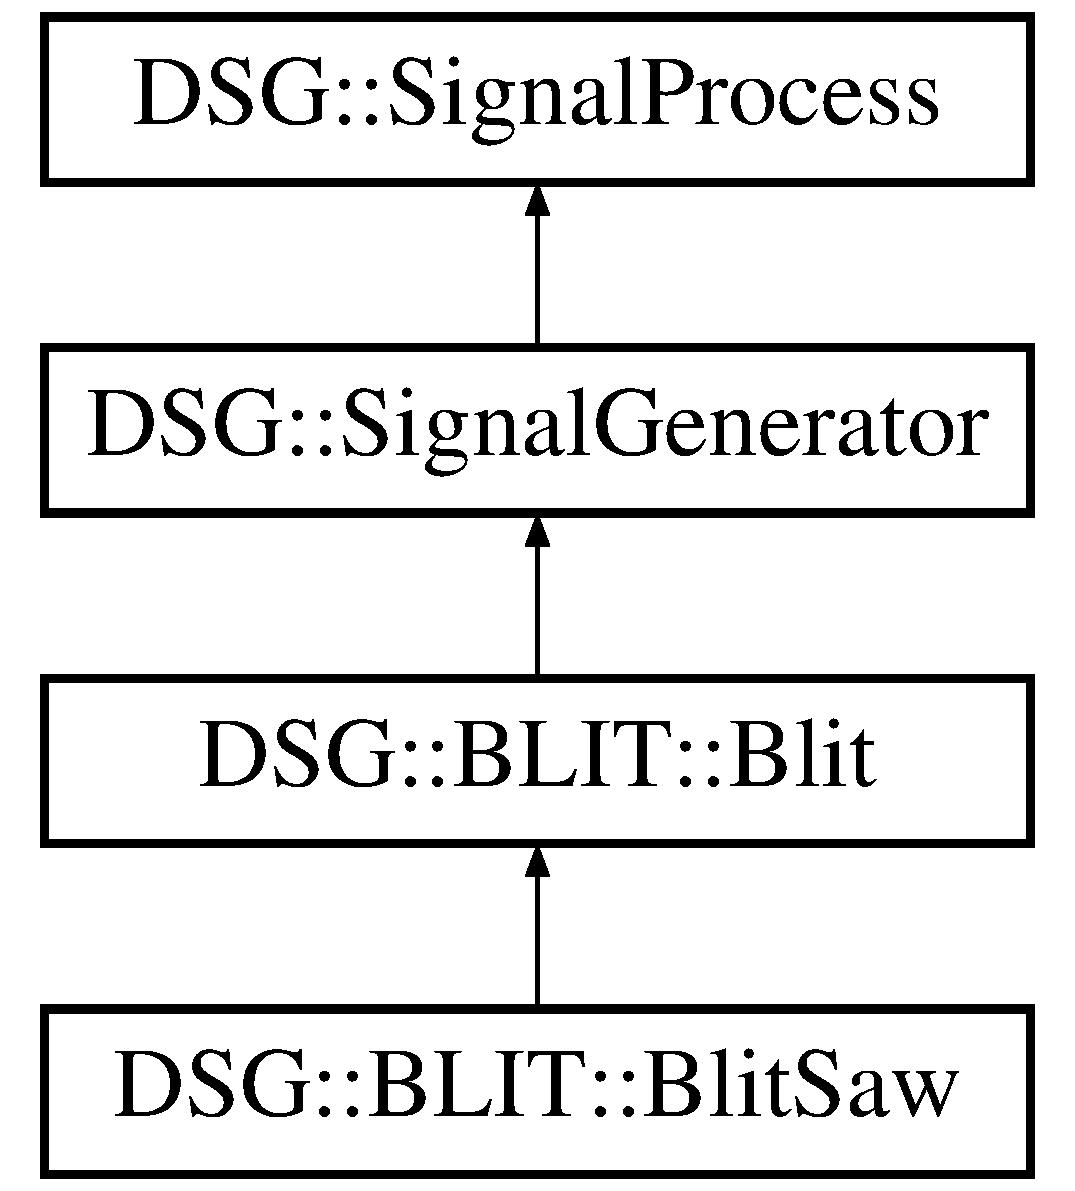
\includegraphics[height=4.000000cm]{class_d_s_g_1_1_b_l_i_t_1_1_blit_saw}
\end{center}
\end{figure}
\subsection*{Public Member Functions}
\begin{DoxyCompactItemize}
\item 
\hyperlink{class_d_s_g_1_1_b_l_i_t_1_1_blit_saw_a5c73a4aeb4df74da4db4896edeb15059}{Blit\+Saw} ()
\item 
\hyperlink{class_d_s_g_1_1_b_l_i_t_1_1_blit_saw_a3d7e4379c00970fa89085ed2c945a2b7}{Blit\+Saw} (\hyperlink{namespace_d_s_g_a4315a061386fa1014fda09b15d3a6973}{D\+S\+G\+::\+D\+S\+G\+Frequency} const \&frequency, \hyperlink{namespace_d_s_g_a44431ce1eb0a7300efdd207bc879e52c}{D\+S\+G\+::\+D\+S\+G\+Phase} const \&offset)
\item 
virtual \hyperlink{class_d_s_g_1_1_b_l_i_t_1_1_blit_saw_a4744c63b29aee896823f19965e11e515}{$\sim$\+Blit\+Saw} ()
\item 
virtual bool \hyperlink{class_d_s_g_1_1_b_l_i_t_1_1_blit_saw_ae24821c51b23b9fe9220a620e558af04}{Perform} (\hyperlink{namespace_d_s_g_ac39a94cd27ebcd9c1e7502d0c624894a}{D\+S\+G\+::\+D\+S\+G\+Sample} \&signal)
\item 
virtual bool \hyperlink{class_d_s_g_1_1_b_l_i_t_1_1_blit_saw_ad2edba8ed83558e76afed6ec1d5cf4d6}{Perform} (\hyperlink{class_d_s_g_1_1_ring_buffer}{D\+S\+G\+::\+Ring\+Buffer} \&signal)
\item 
virtual \hyperlink{namespace_d_s_g_a4315a061386fa1014fda09b15d3a6973}{D\+S\+G\+::\+D\+S\+G\+Frequency} const \& \hyperlink{class_d_s_g_1_1_b_l_i_t_1_1_blit_saw_a290d01796efca84b73eb61a3bc419ebb}{Frequency} (\hyperlink{namespace_d_s_g_a4315a061386fa1014fda09b15d3a6973}{D\+S\+G\+::\+D\+S\+G\+Frequency} const \&\hyperlink{class_d_s_g_1_1_b_l_i_t_1_1_blit_ac8fb9d4fb45d0697bf364bb5d6b570ce}{value})
\end{DoxyCompactItemize}
\subsection*{Protected Attributes}
\begin{DoxyCompactItemize}
\item 
\hyperlink{namespace_d_s_g_ac39a94cd27ebcd9c1e7502d0c624894a}{D\+S\+G\+::\+D\+S\+G\+Sample} \hyperlink{class_d_s_g_1_1_b_l_i_t_1_1_blit_saw_a39ff301ab1f690c070b2045d4a2c40bf}{C2\+\_\+}
\item 
\hyperlink{namespace_d_s_g_ac39a94cd27ebcd9c1e7502d0c624894a}{D\+S\+G\+::\+D\+S\+G\+Sample} \hyperlink{class_d_s_g_1_1_b_l_i_t_1_1_blit_saw_a15da9acffc369dd3c5233c05d37ee488}{Register\+\_\+}
\end{DoxyCompactItemize}
\subsection*{Additional Inherited Members}


\subsection{Detailed Description}
\hyperlink{class_d_s_g_1_1_b_l_i_t_1_1_blit_saw}{D\+S\+G\+::\+B\+L\+I\+T\+::\+Blit\+Saw} -\/ Saw Wave Generator Based on \hyperlink{namespace_d_s_g_1_1_b_l_i_t}{B\+L\+I\+T} Algorithm. 

\begin{DoxyRefDesc}{Todo}
\item[\hyperlink{todo__todo000002}{Todo}]Re-\/write \hyperlink{class_d_s_g_1_1_b_l_i_t_1_1_blit_saw}{D\+S\+G\+::\+B\+L\+I\+T\+::\+Blit\+Saw} algorithm \end{DoxyRefDesc}


Definition at line \hyperlink{_b_l_i_t_saw_8h_source_l00034}{34} of file \hyperlink{_b_l_i_t_saw_8h_source}{B\+L\+I\+T\+Saw.\+h}.



\subsection{Constructor \& Destructor Documentation}
\hypertarget{class_d_s_g_1_1_b_l_i_t_1_1_blit_saw_a5c73a4aeb4df74da4db4896edeb15059}{\index{D\+S\+G\+::\+B\+L\+I\+T\+::\+Blit\+Saw@{D\+S\+G\+::\+B\+L\+I\+T\+::\+Blit\+Saw}!Blit\+Saw@{Blit\+Saw}}
\index{Blit\+Saw@{Blit\+Saw}!D\+S\+G\+::\+B\+L\+I\+T\+::\+Blit\+Saw@{D\+S\+G\+::\+B\+L\+I\+T\+::\+Blit\+Saw}}
\subsubsection[{Blit\+Saw}]{\setlength{\rightskip}{0pt plus 5cm}D\+S\+G\+::\+B\+L\+I\+T\+::\+Blit\+Saw\+::\+Blit\+Saw (
\begin{DoxyParamCaption}
{}
\end{DoxyParamCaption}
)}}\label{class_d_s_g_1_1_b_l_i_t_1_1_blit_saw_a5c73a4aeb4df74da4db4896edeb15059}


Definition at line \hyperlink{_b_l_i_t_saw_8cpp_source_l00025}{25} of file \hyperlink{_b_l_i_t_saw_8cpp_source}{B\+L\+I\+T\+Saw.\+cpp}.


\begin{DoxyCode}
00025                        :\hyperlink{class_d_s_g_1_1_b_l_i_t_1_1_blit}{DSG::BLIT::Blit}(),\hyperlink{class_d_s_g_1_1_b_l_i_t_1_1_blit_saw_a15da9acffc369dd3c5233c05d37ee488}{Register\_}(0)\{
00026     \hyperlink{class_d_s_g_1_1_phasor_a6bdec1d2722e2fa5c7173ac5f7adf682}{Frequency}(0);
00027 \}
\end{DoxyCode}
\hypertarget{class_d_s_g_1_1_b_l_i_t_1_1_blit_saw_a3d7e4379c00970fa89085ed2c945a2b7}{\index{D\+S\+G\+::\+B\+L\+I\+T\+::\+Blit\+Saw@{D\+S\+G\+::\+B\+L\+I\+T\+::\+Blit\+Saw}!Blit\+Saw@{Blit\+Saw}}
\index{Blit\+Saw@{Blit\+Saw}!D\+S\+G\+::\+B\+L\+I\+T\+::\+Blit\+Saw@{D\+S\+G\+::\+B\+L\+I\+T\+::\+Blit\+Saw}}
\subsubsection[{Blit\+Saw}]{\setlength{\rightskip}{0pt plus 5cm}D\+S\+G\+::\+B\+L\+I\+T\+::\+Blit\+Saw\+::\+Blit\+Saw (
\begin{DoxyParamCaption}
\item[{{\bf D\+S\+G\+::\+D\+S\+G\+Frequency} const \&}]{frequency, }
\item[{{\bf D\+S\+G\+::\+D\+S\+G\+Phase} const \&}]{offset}
\end{DoxyParamCaption}
)}}\label{class_d_s_g_1_1_b_l_i_t_1_1_blit_saw_a3d7e4379c00970fa89085ed2c945a2b7}


Definition at line \hyperlink{_b_l_i_t_saw_8cpp_source_l00028}{28} of file \hyperlink{_b_l_i_t_saw_8cpp_source}{B\+L\+I\+T\+Saw.\+cpp}.


\begin{DoxyCode}
00028                                                                                  :
      \hyperlink{class_d_s_g_1_1_b_l_i_t_1_1_blit}{DSG::BLIT::Blit}(frequency,offset),\hyperlink{class_d_s_g_1_1_b_l_i_t_1_1_blit_saw_a15da9acffc369dd3c5233c05d37ee488}{Register\_}(0)\{
00029     \hyperlink{class_d_s_g_1_1_phasor_a6bdec1d2722e2fa5c7173ac5f7adf682}{Frequency}(frequency);
00030 \}
\end{DoxyCode}
\hypertarget{class_d_s_g_1_1_b_l_i_t_1_1_blit_saw_a4744c63b29aee896823f19965e11e515}{\index{D\+S\+G\+::\+B\+L\+I\+T\+::\+Blit\+Saw@{D\+S\+G\+::\+B\+L\+I\+T\+::\+Blit\+Saw}!````~Blit\+Saw@{$\sim$\+Blit\+Saw}}
\index{````~Blit\+Saw@{$\sim$\+Blit\+Saw}!D\+S\+G\+::\+B\+L\+I\+T\+::\+Blit\+Saw@{D\+S\+G\+::\+B\+L\+I\+T\+::\+Blit\+Saw}}
\subsubsection[{$\sim$\+Blit\+Saw}]{\setlength{\rightskip}{0pt plus 5cm}D\+S\+G\+::\+B\+L\+I\+T\+::\+Blit\+Saw\+::$\sim$\+Blit\+Saw (
\begin{DoxyParamCaption}
{}
\end{DoxyParamCaption}
)\hspace{0.3cm}{\ttfamily [virtual]}}}\label{class_d_s_g_1_1_b_l_i_t_1_1_blit_saw_a4744c63b29aee896823f19965e11e515}


Definition at line \hyperlink{_b_l_i_t_saw_8cpp_source_l00031}{31} of file \hyperlink{_b_l_i_t_saw_8cpp_source}{B\+L\+I\+T\+Saw.\+cpp}.


\begin{DoxyCode}
00031 \{\}\end{DoxyCode}


\subsection{Member Function Documentation}
\hypertarget{class_d_s_g_1_1_b_l_i_t_1_1_blit_saw_a290d01796efca84b73eb61a3bc419ebb}{\index{D\+S\+G\+::\+B\+L\+I\+T\+::\+Blit\+Saw@{D\+S\+G\+::\+B\+L\+I\+T\+::\+Blit\+Saw}!Frequency@{Frequency}}
\index{Frequency@{Frequency}!D\+S\+G\+::\+B\+L\+I\+T\+::\+Blit\+Saw@{D\+S\+G\+::\+B\+L\+I\+T\+::\+Blit\+Saw}}
\subsubsection[{Frequency}]{\setlength{\rightskip}{0pt plus 5cm}{\bf D\+S\+G\+::\+D\+S\+G\+Frequency} const \& D\+S\+G\+::\+B\+L\+I\+T\+::\+Blit\+Saw\+::\+Frequency (
\begin{DoxyParamCaption}
\item[{{\bf D\+S\+G\+::\+D\+S\+G\+Frequency} const \&}]{value}
\end{DoxyParamCaption}
)\hspace{0.3cm}{\ttfamily [inline]}, {\ttfamily [virtual]}}}\label{class_d_s_g_1_1_b_l_i_t_1_1_blit_saw_a290d01796efca84b73eb61a3bc419ebb}


Reimplemented from \hyperlink{class_d_s_g_1_1_b_l_i_t_1_1_blit_a933f8f9f324a4fde4f9e2b69473d88ed}{D\+S\+G\+::\+B\+L\+I\+T\+::\+Blit}.



Definition at line \hyperlink{_b_l_i_t_saw_8h_source_l00072}{72} of file \hyperlink{_b_l_i_t_saw_8h_source}{B\+L\+I\+T\+Saw.\+h}.


\begin{DoxyCode}
00072                                                                                            \{
00073             this->\hyperlink{class_d_s_g_1_1_phasor_a6bdec1d2722e2fa5c7173ac5f7adf682}{SignalGenerator::Frequency}(\hyperlink{class_d_s_g_1_1_b_l_i_t_1_1_blit_ac8fb9d4fb45d0697bf364bb5d6b570ce}{value});
00074             \hyperlink{class_d_s_g_1_1_b_l_i_t_1_1_blit_a04d7d6b22a386428e5c25668e1587794}{p\_} = \hyperlink{namespace_d_s_g_a72df05177db0412c3590070923f62819}{DSG::SampleRate}()/\hyperlink{class_d_s_g_1_1_phasor_a85a00065d4445c33fef69eae0ce926df}{\_frequency};
00075             \hyperlink{class_d_s_g_1_1_b_l_i_t_1_1_blit_a632c6f070187969b90c70b65668b82bc}{\_h} = (unsigned)floor(\hyperlink{class_d_s_g_1_1_b_l_i_t_1_1_blit_a04d7d6b22a386428e5c25668e1587794}{p\_}*0.5);
00076             \hyperlink{class_d_s_g_1_1_b_l_i_t_1_1_blit_afa6e4d46efdbfa032762610601ed42a0}{m\_} = 2 * (\hyperlink{class_d_s_g_1_1_b_l_i_t_1_1_blit_a632c6f070187969b90c70b65668b82bc}{\_h})+1;
00077             \hyperlink{class_d_s_g_1_1_b_l_i_t_1_1_blit_a66e2a97840ad0772daaaa9aea63b77b4}{a\_} = \hyperlink{class_d_s_g_1_1_b_l_i_t_1_1_blit_afa6e4d46efdbfa032762610601ed42a0}{m\_}/(double)\hyperlink{class_d_s_g_1_1_b_l_i_t_1_1_blit_a04d7d6b22a386428e5c25668e1587794}{p\_};
00078             \hyperlink{class_d_s_g_1_1_b_l_i_t_1_1_blit_saw_a39ff301ab1f690c070b2045d4a2c40bf}{C2\_} = 1.0/(double)\hyperlink{class_d_s_g_1_1_b_l_i_t_1_1_blit_a04d7d6b22a386428e5c25668e1587794}{p\_};
00079             \textcolor{keywordflow}{return} \hyperlink{class_d_s_g_1_1_phasor_a85a00065d4445c33fef69eae0ce926df}{\_frequency};
00080         \}
\end{DoxyCode}
\hypertarget{class_d_s_g_1_1_b_l_i_t_1_1_blit_saw_ae24821c51b23b9fe9220a620e558af04}{\index{D\+S\+G\+::\+B\+L\+I\+T\+::\+Blit\+Saw@{D\+S\+G\+::\+B\+L\+I\+T\+::\+Blit\+Saw}!Perform@{Perform}}
\index{Perform@{Perform}!D\+S\+G\+::\+B\+L\+I\+T\+::\+Blit\+Saw@{D\+S\+G\+::\+B\+L\+I\+T\+::\+Blit\+Saw}}
\subsubsection[{Perform}]{\setlength{\rightskip}{0pt plus 5cm}bool D\+S\+G\+::\+B\+L\+I\+T\+::\+Blit\+Saw\+::\+Perform (
\begin{DoxyParamCaption}
\item[{{\bf D\+S\+G\+::\+D\+S\+G\+Sample} \&}]{signal}
\end{DoxyParamCaption}
)\hspace{0.3cm}{\ttfamily [inline]}, {\ttfamily [virtual]}}}\label{class_d_s_g_1_1_b_l_i_t_1_1_blit_saw_ae24821c51b23b9fe9220a620e558af04}


Reimplemented from \hyperlink{class_d_s_g_1_1_b_l_i_t_1_1_blit_adfd7c8891b4c4dbd0530a2780781b2bd}{D\+S\+G\+::\+B\+L\+I\+T\+::\+Blit}.



Definition at line \hyperlink{_b_l_i_t_saw_8h_source_l00046}{46} of file \hyperlink{_b_l_i_t_saw_8h_source}{B\+L\+I\+T\+Saw.\+h}.


\begin{DoxyCode}
00046                                                                \{
00047             \hyperlink{class_d_s_g_1_1_b_l_i_t_1_1_blit_a6de89a5a240f226c940aef97661c9cee}{denominator} = \hyperlink{class_d_s_g_1_1_b_l_i_t_1_1_blit_afa6e4d46efdbfa032762610601ed42a0}{m\_} * sin(\hyperlink{_p_i_8h_a598a3330b3c21701223ee0ca14316eca}{PI}*\hyperlink{class_d_s_g_1_1_phasor_a82c148d71128cfc518fc8e7e131c3a38}{\_phasor});
00048             \textcolor{keywordflow}{if} (\hyperlink{namespace_d_s_g_a9eee3c39a1f45d42f0b4fa7201d3ba3d}{DSG::IsDenormal}(\hyperlink{class_d_s_g_1_1_b_l_i_t_1_1_blit_a6de89a5a240f226c940aef97661c9cee}{denominator})) \{
00049                 signal = \hyperlink{class_d_s_g_1_1_b_l_i_t_1_1_blit_a66e2a97840ad0772daaaa9aea63b77b4}{a\_};
00050             \}\textcolor{keywordflow}{else}\{
00051                 \hyperlink{class_d_s_g_1_1_b_l_i_t_1_1_blit_ac8fb9d4fb45d0697bf364bb5d6b570ce}{value} = sin(\hyperlink{_p_i_8h_a598a3330b3c21701223ee0ca14316eca}{PI}*\hyperlink{class_d_s_g_1_1_phasor_a82c148d71128cfc518fc8e7e131c3a38}{\_phasor} * \hyperlink{class_d_s_g_1_1_b_l_i_t_1_1_blit_afa6e4d46efdbfa032762610601ed42a0}{m\_});
00052                 \hyperlink{class_d_s_g_1_1_b_l_i_t_1_1_blit_ac8fb9d4fb45d0697bf364bb5d6b570ce}{value}/=\hyperlink{class_d_s_g_1_1_b_l_i_t_1_1_blit_a6de89a5a240f226c940aef97661c9cee}{denominator};
00053                 \hyperlink{class_d_s_g_1_1_b_l_i_t_1_1_blit_ac8fb9d4fb45d0697bf364bb5d6b570ce}{value}*=\hyperlink{class_d_s_g_1_1_b_l_i_t_1_1_blit_a66e2a97840ad0772daaaa9aea63b77b4}{a\_};
00054                 signal = \hyperlink{class_d_s_g_1_1_b_l_i_t_1_1_blit_ac8fb9d4fb45d0697bf364bb5d6b570ce}{value};
00055             \}
00056             \hyperlink{class_d_s_g_1_1_phasor_a6a088b29e506fb5e99d73f4f0160c583}{step}();
00057             signal += (\hyperlink{class_d_s_g_1_1_b_l_i_t_1_1_blit_saw_a15da9acffc369dd3c5233c05d37ee488}{Register\_} - \hyperlink{class_d_s_g_1_1_b_l_i_t_1_1_blit_saw_a39ff301ab1f690c070b2045d4a2c40bf}{C2\_});
00058             \hyperlink{class_d_s_g_1_1_b_l_i_t_1_1_blit_saw_a15da9acffc369dd3c5233c05d37ee488}{Register\_} = signal * 0.995;
00059             \hyperlink{class_d_s_g_1_1_b_l_i_t_1_1_blit_saw_a39ff301ab1f690c070b2045d4a2c40bf}{C2\_}+=signal;
00060             \hyperlink{class_d_s_g_1_1_b_l_i_t_1_1_blit_saw_a39ff301ab1f690c070b2045d4a2c40bf}{C2\_}*=0.5;
00061             \textcolor{keywordflow}{return} \textcolor{keyword}{true};
00062         \}
\end{DoxyCode}
\hypertarget{class_d_s_g_1_1_b_l_i_t_1_1_blit_saw_ad2edba8ed83558e76afed6ec1d5cf4d6}{\index{D\+S\+G\+::\+B\+L\+I\+T\+::\+Blit\+Saw@{D\+S\+G\+::\+B\+L\+I\+T\+::\+Blit\+Saw}!Perform@{Perform}}
\index{Perform@{Perform}!D\+S\+G\+::\+B\+L\+I\+T\+::\+Blit\+Saw@{D\+S\+G\+::\+B\+L\+I\+T\+::\+Blit\+Saw}}
\subsubsection[{Perform}]{\setlength{\rightskip}{0pt plus 5cm}bool D\+S\+G\+::\+B\+L\+I\+T\+::\+Blit\+Saw\+::\+Perform (
\begin{DoxyParamCaption}
\item[{{\bf D\+S\+G\+::\+Ring\+Buffer} \&}]{signal}
\end{DoxyParamCaption}
)\hspace{0.3cm}{\ttfamily [inline]}, {\ttfamily [virtual]}}}\label{class_d_s_g_1_1_b_l_i_t_1_1_blit_saw_ad2edba8ed83558e76afed6ec1d5cf4d6}


Reimplemented from \hyperlink{class_d_s_g_1_1_b_l_i_t_1_1_blit_aab7c67ff8f059c8367ba316cf8cd5436}{D\+S\+G\+::\+B\+L\+I\+T\+::\+Blit}.



Definition at line \hyperlink{_b_l_i_t_saw_8h_source_l00063}{63} of file \hyperlink{_b_l_i_t_saw_8h_source}{B\+L\+I\+T\+Saw.\+h}.


\begin{DoxyCode}
00063                                                                 \{
00064             signal.\hyperlink{class_d_s_g_1_1_ring_buffer_ab23c8003d2857809a816068eeb209d60}{Flush}();
00065             \textcolor{keywordflow}{while} (!signal.\hyperlink{class_d_s_g_1_1_ring_buffer_a53ddb04ffcbb5470a8d2b0a3c65b70cb}{Full}()) \{
00066                 \textcolor{keywordflow}{if} (\hyperlink{class_d_s_g_1_1_b_l_i_t_1_1_blit_saw_ae24821c51b23b9fe9220a620e558af04}{Perform}(\hyperlink{class_d_s_g_1_1_signal_generator_a28a9b47a1aa0783029f11a19ba0363f2}{\_storage})) \{
00067                     \textcolor{keywordflow}{if}(signal.\hyperlink{class_d_s_g_1_1_ring_buffer_aa5dd2caa0a270173251faee40a43d692}{Write}(\hyperlink{class_d_s_g_1_1_signal_generator_a28a9b47a1aa0783029f11a19ba0363f2}{\_storage}))\{
00068                     \}\textcolor{keywordflow}{else} \textcolor{keywordflow}{return} \textcolor{keyword}{false};
00069                 \}\textcolor{keywordflow}{else} \textcolor{keywordflow}{return} \textcolor{keyword}{false};
00070             \}\textcolor{keywordflow}{return} \textcolor{keyword}{true};
00071         \}
\end{DoxyCode}


\subsection{Member Data Documentation}
\hypertarget{class_d_s_g_1_1_b_l_i_t_1_1_blit_saw_a39ff301ab1f690c070b2045d4a2c40bf}{\index{D\+S\+G\+::\+B\+L\+I\+T\+::\+Blit\+Saw@{D\+S\+G\+::\+B\+L\+I\+T\+::\+Blit\+Saw}!C2\+\_\+@{C2\+\_\+}}
\index{C2\+\_\+@{C2\+\_\+}!D\+S\+G\+::\+B\+L\+I\+T\+::\+Blit\+Saw@{D\+S\+G\+::\+B\+L\+I\+T\+::\+Blit\+Saw}}
\subsubsection[{C2\+\_\+}]{\setlength{\rightskip}{0pt plus 5cm}{\bf D\+S\+G\+::\+D\+S\+G\+Sample} D\+S\+G\+::\+B\+L\+I\+T\+::\+Blit\+Saw\+::\+C2\+\_\+\hspace{0.3cm}{\ttfamily [protected]}}}\label{class_d_s_g_1_1_b_l_i_t_1_1_blit_saw_a39ff301ab1f690c070b2045d4a2c40bf}


Definition at line \hyperlink{_b_l_i_t_saw_8h_source_l00043}{43} of file \hyperlink{_b_l_i_t_saw_8h_source}{B\+L\+I\+T\+Saw.\+h}.

\hypertarget{class_d_s_g_1_1_b_l_i_t_1_1_blit_saw_a15da9acffc369dd3c5233c05d37ee488}{\index{D\+S\+G\+::\+B\+L\+I\+T\+::\+Blit\+Saw@{D\+S\+G\+::\+B\+L\+I\+T\+::\+Blit\+Saw}!Register\+\_\+@{Register\+\_\+}}
\index{Register\+\_\+@{Register\+\_\+}!D\+S\+G\+::\+B\+L\+I\+T\+::\+Blit\+Saw@{D\+S\+G\+::\+B\+L\+I\+T\+::\+Blit\+Saw}}
\subsubsection[{Register\+\_\+}]{\setlength{\rightskip}{0pt plus 5cm}{\bf D\+S\+G\+::\+D\+S\+G\+Sample} D\+S\+G\+::\+B\+L\+I\+T\+::\+Blit\+Saw\+::\+Register\+\_\+\hspace{0.3cm}{\ttfamily [protected]}}}\label{class_d_s_g_1_1_b_l_i_t_1_1_blit_saw_a15da9acffc369dd3c5233c05d37ee488}


Definition at line \hyperlink{_b_l_i_t_saw_8h_source_l00044}{44} of file \hyperlink{_b_l_i_t_saw_8h_source}{B\+L\+I\+T\+Saw.\+h}.



The documentation for this class was generated from the following files\+:\begin{DoxyCompactItemize}
\item 
\hyperlink{_b_l_i_t_saw_8h}{B\+L\+I\+T\+Saw.\+h}\item 
\hyperlink{_b_l_i_t_saw_8cpp}{B\+L\+I\+T\+Saw.\+cpp}\end{DoxyCompactItemize}

\hypertarget{class_d_s_g_1_1_buffer}{\section{D\+S\+G\+:\+:Buffer Class Reference}
\label{class_d_s_g_1_1_buffer}\index{D\+S\+G\+::\+Buffer@{D\+S\+G\+::\+Buffer}}
}


\hyperlink{class_d_s_g_1_1_buffer}{D\+S\+G\+::\+Buffer} -\/ Base Class For \hyperlink{class_d_s_g_1_1_ring_buffer}{D\+S\+G\+::\+Ring\+Buffer}. Not For Direct Use.  




{\ttfamily \#include $<$Buffer.\+h$>$}

Inheritance diagram for D\+S\+G\+:\+:Buffer\+:\begin{figure}[H]
\begin{center}
\leavevmode
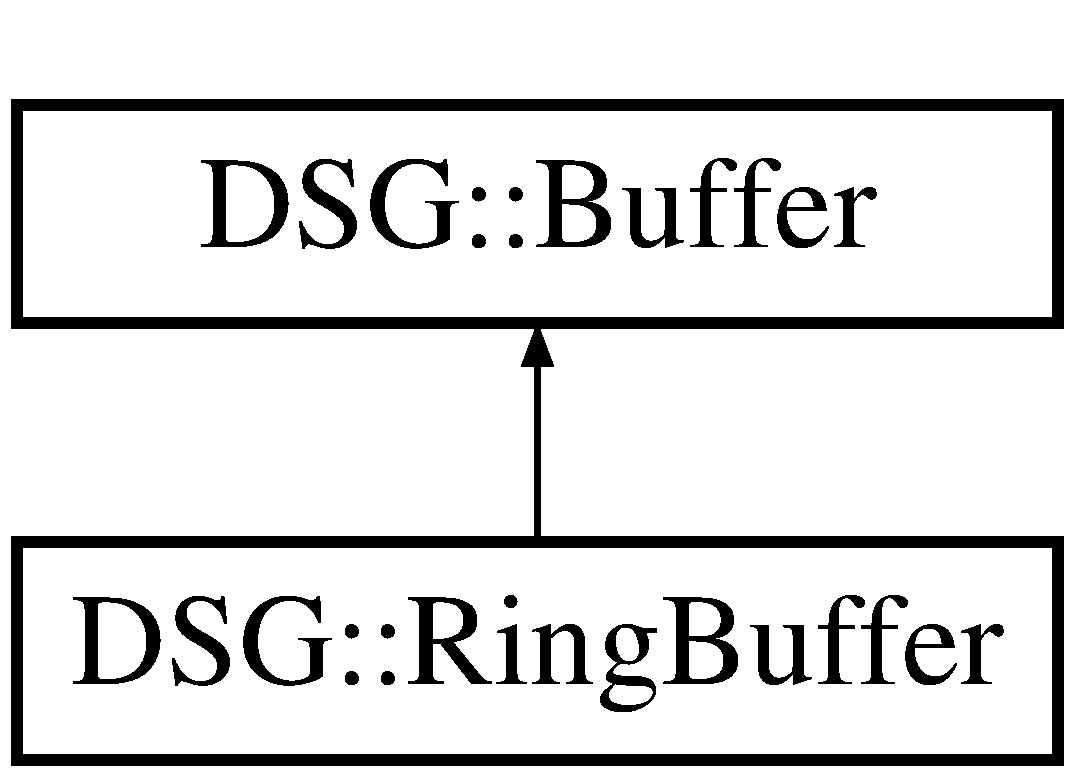
\includegraphics[height=2.000000cm]{class_d_s_g_1_1_buffer}
\end{center}
\end{figure}
\subsection*{Public Member Functions}
\begin{DoxyCompactItemize}
\item 
\hyperlink{class_d_s_g_1_1_buffer_aa764dd8c389dcff51de08cb81fafeb86}{Buffer} ()
\item 
\hyperlink{class_d_s_g_1_1_buffer_a0e6502fd61833043744f9df94e8d5111}{Buffer} (size\+\_\+t size)
\item 
\hyperlink{class_d_s_g_1_1_buffer_a468a65d70553dfb773e4592b4b077683}{Buffer} (\hyperlink{class_d_s_g_1_1_buffer}{Buffer} const \&other)
\item 
\hyperlink{class_d_s_g_1_1_buffer}{Buffer} \& \hyperlink{class_d_s_g_1_1_buffer_a977d572a7d402ff6bf991d7c5c0cc6a7}{operator=} (\hyperlink{class_d_s_g_1_1_buffer}{Buffer} const \&other)
\item 
virtual \hyperlink{class_d_s_g_1_1_buffer_a619fc41bf263a419da1a19254e194101}{$\sim$\+Buffer} ()
\item 
\hyperlink{namespace_d_s_g_ac39a94cd27ebcd9c1e7502d0c624894a}{D\+S\+G\+::\+D\+S\+G\+Sample} \& \hyperlink{class_d_s_g_1_1_buffer_a5358d81096cd0801e4fce7851809b3ef}{operator\mbox{[}$\,$\mbox{]}} (size\+\_\+t const \&index)
\item 
size\+\_\+t const \& \hyperlink{class_d_s_g_1_1_buffer_a4acea659d9cd0be652ec55d21e5b0262}{Size} () const 
\end{DoxyCompactItemize}
\subsection*{Protected Attributes}
\begin{DoxyCompactItemize}
\item 
\hyperlink{namespace_d_s_g_ac39a94cd27ebcd9c1e7502d0c624894a}{D\+S\+G\+::\+D\+S\+G\+Sample} $\ast$ \hyperlink{class_d_s_g_1_1_buffer_ae4a4db8fe44b62db18d6a7855b5773f9}{\+\_\+buffer}
\item 
size\+\_\+t \hyperlink{class_d_s_g_1_1_buffer_a4e2fef9ed617af2554b25c999def8f71}{\+\_\+size}
\end{DoxyCompactItemize}


\subsection{Detailed Description}
\hyperlink{class_d_s_g_1_1_buffer}{D\+S\+G\+::\+Buffer} -\/ Base Class For \hyperlink{class_d_s_g_1_1_ring_buffer}{D\+S\+G\+::\+Ring\+Buffer}. Not For Direct Use. 

Definition at line \hyperlink{_buffer_8h_source_l00018}{18} of file \hyperlink{_buffer_8h_source}{Buffer.\+h}.



\subsection{Constructor \& Destructor Documentation}
\hypertarget{class_d_s_g_1_1_buffer_aa764dd8c389dcff51de08cb81fafeb86}{\index{D\+S\+G\+::\+Buffer@{D\+S\+G\+::\+Buffer}!Buffer@{Buffer}}
\index{Buffer@{Buffer}!D\+S\+G\+::\+Buffer@{D\+S\+G\+::\+Buffer}}
\subsubsection[{Buffer}]{\setlength{\rightskip}{0pt plus 5cm}D\+S\+G\+::\+Buffer\+::\+Buffer (
\begin{DoxyParamCaption}
{}
\end{DoxyParamCaption}
)}}\label{class_d_s_g_1_1_buffer_aa764dd8c389dcff51de08cb81fafeb86}


Definition at line \hyperlink{_buffer_8cpp_source_l00009}{9} of file \hyperlink{_buffer_8cpp_source}{Buffer.\+cpp}.


\begin{DoxyCode}
00009 :\hyperlink{class_d_s_g_1_1_buffer_a4e2fef9ed617af2554b25c999def8f71}{\_size}(0),\hyperlink{class_d_s_g_1_1_buffer_ae4a4db8fe44b62db18d6a7855b5773f9}{\_buffer}(\textcolor{keyword}{nullptr})\{\}
\end{DoxyCode}
\hypertarget{class_d_s_g_1_1_buffer_a0e6502fd61833043744f9df94e8d5111}{\index{D\+S\+G\+::\+Buffer@{D\+S\+G\+::\+Buffer}!Buffer@{Buffer}}
\index{Buffer@{Buffer}!D\+S\+G\+::\+Buffer@{D\+S\+G\+::\+Buffer}}
\subsubsection[{Buffer}]{\setlength{\rightskip}{0pt plus 5cm}D\+S\+G\+::\+Buffer\+::\+Buffer (
\begin{DoxyParamCaption}
\item[{size\+\_\+t}]{size}
\end{DoxyParamCaption}
)}}\label{class_d_s_g_1_1_buffer_a0e6502fd61833043744f9df94e8d5111}


Definition at line \hyperlink{_buffer_8cpp_source_l00010}{10} of file \hyperlink{_buffer_8cpp_source}{Buffer.\+cpp}.


\begin{DoxyCode}
00010 :\hyperlink{class_d_s_g_1_1_buffer_a4e2fef9ed617af2554b25c999def8f71}{\_size}(size),\hyperlink{class_d_s_g_1_1_buffer_ae4a4db8fe44b62db18d6a7855b5773f9}{\_buffer}(\textcolor{keyword}{new} \hyperlink{namespace_d_s_g_ac39a94cd27ebcd9c1e7502d0c624894a}{DSG::DSGSample}[size])\{\}
\end{DoxyCode}
\hypertarget{class_d_s_g_1_1_buffer_a468a65d70553dfb773e4592b4b077683}{\index{D\+S\+G\+::\+Buffer@{D\+S\+G\+::\+Buffer}!Buffer@{Buffer}}
\index{Buffer@{Buffer}!D\+S\+G\+::\+Buffer@{D\+S\+G\+::\+Buffer}}
\subsubsection[{Buffer}]{\setlength{\rightskip}{0pt plus 5cm}D\+S\+G\+::\+Buffer\+::\+Buffer (
\begin{DoxyParamCaption}
\item[{{\bf Buffer} const \&}]{other}
\end{DoxyParamCaption}
)}}\label{class_d_s_g_1_1_buffer_a468a65d70553dfb773e4592b4b077683}


Definition at line \hyperlink{_buffer_8cpp_source_l00011}{11} of file \hyperlink{_buffer_8cpp_source}{Buffer.\+cpp}.


\begin{DoxyCode}
00011                                      \{
00012     \hyperlink{class_d_s_g_1_1_buffer_ae4a4db8fe44b62db18d6a7855b5773f9}{\_buffer} = \textcolor{keyword}{new}  \hyperlink{namespace_d_s_g_ac39a94cd27ebcd9c1e7502d0c624894a}{DSG::DSGSample}[\hyperlink{class_d_s_g_1_1_buffer_a4e2fef9ed617af2554b25c999def8f71}{\_size}];
00013     \hyperlink{class_d_s_g_1_1_buffer_a4e2fef9ed617af2554b25c999def8f71}{\_size} = other.\_size;
00014     *\textcolor{keyword}{this} = other;
00015 \}
\end{DoxyCode}
\hypertarget{class_d_s_g_1_1_buffer_a619fc41bf263a419da1a19254e194101}{\index{D\+S\+G\+::\+Buffer@{D\+S\+G\+::\+Buffer}!````~Buffer@{$\sim$\+Buffer}}
\index{````~Buffer@{$\sim$\+Buffer}!D\+S\+G\+::\+Buffer@{D\+S\+G\+::\+Buffer}}
\subsubsection[{$\sim$\+Buffer}]{\setlength{\rightskip}{0pt plus 5cm}D\+S\+G\+::\+Buffer\+::$\sim$\+Buffer (
\begin{DoxyParamCaption}
{}
\end{DoxyParamCaption}
)\hspace{0.3cm}{\ttfamily [virtual]}}}\label{class_d_s_g_1_1_buffer_a619fc41bf263a419da1a19254e194101}


Definition at line \hyperlink{_buffer_8cpp_source_l00029}{29} of file \hyperlink{_buffer_8cpp_source}{Buffer.\+cpp}.


\begin{DoxyCode}
00029                   \{
00030     \textcolor{keywordflow}{if} (\hyperlink{class_d_s_g_1_1_buffer_ae4a4db8fe44b62db18d6a7855b5773f9}{\_buffer}!=\textcolor{keyword}{nullptr}) \{
00031         \textcolor{keyword}{delete} [] \hyperlink{class_d_s_g_1_1_buffer_ae4a4db8fe44b62db18d6a7855b5773f9}{\_buffer};
00032     \}
00033 \}
\end{DoxyCode}


\subsection{Member Function Documentation}
\hypertarget{class_d_s_g_1_1_buffer_a977d572a7d402ff6bf991d7c5c0cc6a7}{\index{D\+S\+G\+::\+Buffer@{D\+S\+G\+::\+Buffer}!operator=@{operator=}}
\index{operator=@{operator=}!D\+S\+G\+::\+Buffer@{D\+S\+G\+::\+Buffer}}
\subsubsection[{operator=}]{\setlength{\rightskip}{0pt plus 5cm}{\bf D\+S\+G\+::\+Buffer} \& D\+S\+G\+::\+Buffer\+::operator= (
\begin{DoxyParamCaption}
\item[{{\bf Buffer} const \&}]{other}
\end{DoxyParamCaption}
)}}\label{class_d_s_g_1_1_buffer_a977d572a7d402ff6bf991d7c5c0cc6a7}


Definition at line \hyperlink{_buffer_8cpp_source_l00016}{16} of file \hyperlink{_buffer_8cpp_source}{Buffer.\+cpp}.


\begin{DoxyCode}
00016                                                   \{
00017     \textcolor{keywordflow}{if} (\hyperlink{class_d_s_g_1_1_buffer_a4e2fef9ed617af2554b25c999def8f71}{\_size}!=other.\_size) \{
00018         \textcolor{keywordflow}{if} (\hyperlink{class_d_s_g_1_1_buffer_ae4a4db8fe44b62db18d6a7855b5773f9}{\_buffer}!=\textcolor{keyword}{nullptr}) \{
00019             \textcolor{keyword}{delete} [] \hyperlink{class_d_s_g_1_1_buffer_ae4a4db8fe44b62db18d6a7855b5773f9}{\_buffer};
00020         \}
00021         \hyperlink{class_d_s_g_1_1_buffer_a4e2fef9ed617af2554b25c999def8f71}{\_size} = other.\_size;
00022         \hyperlink{class_d_s_g_1_1_buffer_ae4a4db8fe44b62db18d6a7855b5773f9}{\_buffer} = \textcolor{keyword}{new}  \hyperlink{namespace_d_s_g_ac39a94cd27ebcd9c1e7502d0c624894a}{DSG::DSGSample}[\hyperlink{class_d_s_g_1_1_buffer_a4e2fef9ed617af2554b25c999def8f71}{\_size}];
00023     \}
00024     \textcolor{keywordflow}{for} (\textcolor{keywordtype}{int} i=0; i<\hyperlink{class_d_s_g_1_1_buffer_a4e2fef9ed617af2554b25c999def8f71}{\_size}; ++i) \{
00025         \hyperlink{class_d_s_g_1_1_buffer_ae4a4db8fe44b62db18d6a7855b5773f9}{\_buffer}[i] = other.\_buffer[i];
00026     \}
00027     \textcolor{keywordflow}{return} *\textcolor{keyword}{this};
00028 \}
\end{DoxyCode}
\hypertarget{class_d_s_g_1_1_buffer_a5358d81096cd0801e4fce7851809b3ef}{\index{D\+S\+G\+::\+Buffer@{D\+S\+G\+::\+Buffer}!operator\mbox{[}$\,$\mbox{]}@{operator[]}}
\index{operator\mbox{[}$\,$\mbox{]}@{operator[]}!D\+S\+G\+::\+Buffer@{D\+S\+G\+::\+Buffer}}
\subsubsection[{operator[]}]{\setlength{\rightskip}{0pt plus 5cm}{\bf D\+S\+G\+::\+D\+S\+G\+Sample} \& D\+S\+G\+::\+Buffer\+::operator\mbox{[}$\,$\mbox{]} (
\begin{DoxyParamCaption}
\item[{size\+\_\+t const \&}]{index}
\end{DoxyParamCaption}
)}}\label{class_d_s_g_1_1_buffer_a5358d81096cd0801e4fce7851809b3ef}


Definition at line \hyperlink{_buffer_8cpp_source_l00034}{34} of file \hyperlink{_buffer_8cpp_source}{Buffer.\+cpp}.


\begin{DoxyCode}
00034                                                       \{
00035 \textcolor{preprocessor}{#ifdef DEBUG}
00036     assert(index<\hyperlink{class_d_s_g_1_1_buffer_a4e2fef9ed617af2554b25c999def8f71}{\_size});
00037 \textcolor{preprocessor}{#endif}
00038     \textcolor{keywordflow}{return} \hyperlink{class_d_s_g_1_1_buffer_ae4a4db8fe44b62db18d6a7855b5773f9}{\_buffer}[index];
00039 \}\end{DoxyCode}
\hypertarget{class_d_s_g_1_1_buffer_a4acea659d9cd0be652ec55d21e5b0262}{\index{D\+S\+G\+::\+Buffer@{D\+S\+G\+::\+Buffer}!Size@{Size}}
\index{Size@{Size}!D\+S\+G\+::\+Buffer@{D\+S\+G\+::\+Buffer}}
\subsubsection[{Size}]{\setlength{\rightskip}{0pt plus 5cm}size\+\_\+t const \& D\+S\+G\+::\+Buffer\+::\+Size (
\begin{DoxyParamCaption}
{}
\end{DoxyParamCaption}
) const\hspace{0.3cm}{\ttfamily [inline]}}}\label{class_d_s_g_1_1_buffer_a4acea659d9cd0be652ec55d21e5b0262}


Definition at line \hyperlink{_buffer_8h_source_l00031}{31} of file \hyperlink{_buffer_8h_source}{Buffer.\+h}.


\begin{DoxyCode}
00031                                              \{
00032         \textcolor{keywordflow}{return} \hyperlink{class_d_s_g_1_1_buffer_a4e2fef9ed617af2554b25c999def8f71}{\_size};
00033     \}
\end{DoxyCode}


\subsection{Member Data Documentation}
\hypertarget{class_d_s_g_1_1_buffer_ae4a4db8fe44b62db18d6a7855b5773f9}{\index{D\+S\+G\+::\+Buffer@{D\+S\+G\+::\+Buffer}!\+\_\+buffer@{\+\_\+buffer}}
\index{\+\_\+buffer@{\+\_\+buffer}!D\+S\+G\+::\+Buffer@{D\+S\+G\+::\+Buffer}}
\subsubsection[{\+\_\+buffer}]{\setlength{\rightskip}{0pt plus 5cm}{\bf D\+S\+G\+::\+D\+S\+G\+Sample}$\ast$ D\+S\+G\+::\+Buffer\+::\+\_\+buffer\hspace{0.3cm}{\ttfamily [protected]}}}\label{class_d_s_g_1_1_buffer_ae4a4db8fe44b62db18d6a7855b5773f9}


Definition at line \hyperlink{_buffer_8h_source_l00028}{28} of file \hyperlink{_buffer_8h_source}{Buffer.\+h}.

\hypertarget{class_d_s_g_1_1_buffer_a4e2fef9ed617af2554b25c999def8f71}{\index{D\+S\+G\+::\+Buffer@{D\+S\+G\+::\+Buffer}!\+\_\+size@{\+\_\+size}}
\index{\+\_\+size@{\+\_\+size}!D\+S\+G\+::\+Buffer@{D\+S\+G\+::\+Buffer}}
\subsubsection[{\+\_\+size}]{\setlength{\rightskip}{0pt plus 5cm}size\+\_\+t D\+S\+G\+::\+Buffer\+::\+\_\+size\hspace{0.3cm}{\ttfamily [protected]}}}\label{class_d_s_g_1_1_buffer_a4e2fef9ed617af2554b25c999def8f71}


Definition at line \hyperlink{_buffer_8h_source_l00029}{29} of file \hyperlink{_buffer_8h_source}{Buffer.\+h}.



The documentation for this class was generated from the following files\+:\begin{DoxyCompactItemize}
\item 
/\+Users/alexanderzywicki/\+Documents/\+D\+S\+G/src/\hyperlink{_buffer_8h}{Buffer.\+h}\item 
/\+Users/alexanderzywicki/\+Documents/\+D\+S\+G/src/\hyperlink{_buffer_8cpp}{Buffer.\+cpp}\end{DoxyCompactItemize}

\hypertarget{class_d_s_g_1_1_fourier_1_1_fourier_saw}{\section{D\+S\+G\+:\+:Fourier\+:\+:Fourier\+Saw Class Reference}
\label{class_d_s_g_1_1_fourier_1_1_fourier_saw}\index{D\+S\+G\+::\+Fourier\+::\+Fourier\+Saw@{D\+S\+G\+::\+Fourier\+::\+Fourier\+Saw}}
}


\hyperlink{class_d_s_g_1_1_fourier_1_1_fourier_saw}{D\+S\+G\+::\+Fourier\+::\+Fourier\+Saw} -\/ \hyperlink{namespace_d_s_g_1_1_fourier}{Fourier} Series Sawtooth Wave Generator.  




{\ttfamily \#include $<$Fourier\+Saw.\+h$>$}

Inheritance diagram for D\+S\+G\+:\+:Fourier\+:\+:Fourier\+Saw\+:\begin{figure}[H]
\begin{center}
\leavevmode
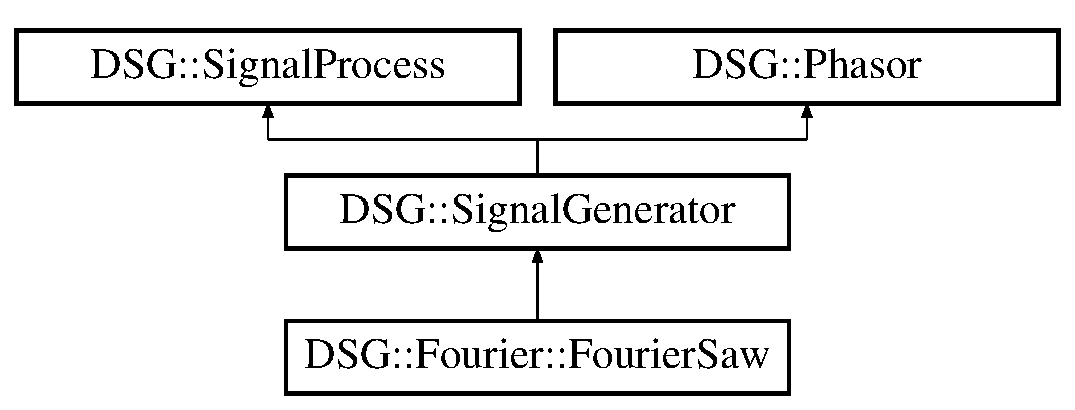
\includegraphics[height=3.000000cm]{class_d_s_g_1_1_fourier_1_1_fourier_saw}
\end{center}
\end{figure}
\subsection*{Public Member Functions}
\begin{DoxyCompactItemize}
\item 
\hyperlink{class_d_s_g_1_1_fourier_1_1_fourier_saw_acfef03c4384ef656110c51102e346c49}{Fourier\+Saw} ()
\item 
\hyperlink{class_d_s_g_1_1_fourier_1_1_fourier_saw_a6062c388900f32e1cfd6df95b9760065}{Fourier\+Saw} (\hyperlink{namespace_d_s_g_a4315a061386fa1014fda09b15d3a6973}{D\+S\+G\+::\+D\+S\+G\+Frequency} const \&frequency, \hyperlink{namespace_d_s_g_a44431ce1eb0a7300efdd207bc879e52c}{D\+S\+G\+::\+D\+S\+G\+Phase} const \&offset)
\item 
virtual \hyperlink{class_d_s_g_1_1_fourier_1_1_fourier_saw_acd28c4942553271ed9f39e8f05b8db6d}{$\sim$\+Fourier\+Saw} ()
\item 
virtual bool \hyperlink{class_d_s_g_1_1_fourier_1_1_fourier_saw_a33061612ff24180f12e9a2c29dfaa116}{Perform} (\hyperlink{namespace_d_s_g_ac39a94cd27ebcd9c1e7502d0c624894a}{D\+S\+G\+::\+D\+S\+G\+Sample} \&signal)
\item 
virtual bool \hyperlink{class_d_s_g_1_1_fourier_1_1_fourier_saw_ac890d9f0af523b63b96b07e6696a32b7}{Perform} (\hyperlink{class_d_s_g_1_1_ring_buffer}{D\+S\+G\+::\+Ring\+Buffer} \&signal)
\item 
virtual \hyperlink{namespace_d_s_g_a4315a061386fa1014fda09b15d3a6973}{D\+S\+G\+::\+D\+S\+G\+Frequency} const \& \hyperlink{class_d_s_g_1_1_fourier_1_1_fourier_saw_afa3d86f404be3665f10c74fe9286ef10}{Frequency} (\hyperlink{namespace_d_s_g_a4315a061386fa1014fda09b15d3a6973}{D\+S\+G\+::\+D\+S\+G\+Frequency} const \&\hyperlink{class_d_s_g_1_1_fourier_1_1_fourier_saw_a97d69a0c03cfb66b1cf6e13fe7073c12}{value})
\end{DoxyCompactItemize}
\subsection*{Protected Attributes}
\begin{DoxyCompactItemize}
\item 
unsigned long \hyperlink{class_d_s_g_1_1_fourier_1_1_fourier_saw_a78d30240b7eb99fcb249b5aafe3d55b2}{\+\_\+h}
\item 
const double \hyperlink{class_d_s_g_1_1_fourier_1_1_fourier_saw_a54895160b61b8d84dc967e7815d07869}{\+\_\+a}
\item 
double \hyperlink{class_d_s_g_1_1_fourier_1_1_fourier_saw_a5df3e5b00224924e106ffdc1d0b6a3cc}{phs}
\item 
double \hyperlink{class_d_s_g_1_1_fourier_1_1_fourier_saw_a97d69a0c03cfb66b1cf6e13fe7073c12}{value}
\item 
int \hyperlink{class_d_s_g_1_1_fourier_1_1_fourier_saw_a261b19d0082558b6e1bb128d267c400d}{i}
\end{DoxyCompactItemize}
\subsection*{Additional Inherited Members}


\subsection{Detailed Description}
\hyperlink{class_d_s_g_1_1_fourier_1_1_fourier_saw}{D\+S\+G\+::\+Fourier\+::\+Fourier\+Saw} -\/ \hyperlink{namespace_d_s_g_1_1_fourier}{Fourier} Series Sawtooth Wave Generator. 

Definition at line \hyperlink{_fourier_saw_8h_source_l00018}{18} of file \hyperlink{_fourier_saw_8h_source}{Fourier\+Saw.\+h}.



\subsection{Constructor \& Destructor Documentation}
\hypertarget{class_d_s_g_1_1_fourier_1_1_fourier_saw_acfef03c4384ef656110c51102e346c49}{\index{D\+S\+G\+::\+Fourier\+::\+Fourier\+Saw@{D\+S\+G\+::\+Fourier\+::\+Fourier\+Saw}!Fourier\+Saw@{Fourier\+Saw}}
\index{Fourier\+Saw@{Fourier\+Saw}!D\+S\+G\+::\+Fourier\+::\+Fourier\+Saw@{D\+S\+G\+::\+Fourier\+::\+Fourier\+Saw}}
\subsubsection[{Fourier\+Saw}]{\setlength{\rightskip}{0pt plus 5cm}D\+S\+G\+::\+Fourier\+::\+Fourier\+Saw\+::\+Fourier\+Saw (
\begin{DoxyParamCaption}
{}
\end{DoxyParamCaption}
)}}\label{class_d_s_g_1_1_fourier_1_1_fourier_saw_acfef03c4384ef656110c51102e346c49}


Definition at line \hyperlink{_fourier_saw_8cpp_source_l00009}{9} of file \hyperlink{_fourier_saw_8cpp_source}{Fourier\+Saw.\+cpp}.


\begin{DoxyCode}
00009 :\hyperlink{class_d_s_g_1_1_signal_generator}{DSG::SignalGenerator}(),\hyperlink{class_d_s_g_1_1_fourier_1_1_fourier_saw_a54895160b61b8d84dc967e7815d07869}{\_a}(1.7/\hyperlink{_p_i_8h_a598a3330b3c21701223ee0ca14316eca}{PI}),\hyperlink{class_d_s_g_1_1_fourier_1_1_fourier_saw_a5df3e5b00224924e106ffdc1d0b6a3cc}{phs}(0),\hyperlink{class_d_s_g_1_1_fourier_1_1_fourier_saw_a97d69a0c03cfb66b1cf6e13fe7073c12}{value}(0),
      \hyperlink{class_d_s_g_1_1_fourier_1_1_fourier_saw_a261b19d0082558b6e1bb128d267c400d}{i}(0)\{\}
\end{DoxyCode}
\hypertarget{class_d_s_g_1_1_fourier_1_1_fourier_saw_a6062c388900f32e1cfd6df95b9760065}{\index{D\+S\+G\+::\+Fourier\+::\+Fourier\+Saw@{D\+S\+G\+::\+Fourier\+::\+Fourier\+Saw}!Fourier\+Saw@{Fourier\+Saw}}
\index{Fourier\+Saw@{Fourier\+Saw}!D\+S\+G\+::\+Fourier\+::\+Fourier\+Saw@{D\+S\+G\+::\+Fourier\+::\+Fourier\+Saw}}
\subsubsection[{Fourier\+Saw}]{\setlength{\rightskip}{0pt plus 5cm}D\+S\+G\+::\+Fourier\+::\+Fourier\+Saw\+::\+Fourier\+Saw (
\begin{DoxyParamCaption}
\item[{{\bf D\+S\+G\+::\+D\+S\+G\+Frequency} const \&}]{frequency, }
\item[{{\bf D\+S\+G\+::\+D\+S\+G\+Phase} const \&}]{offset}
\end{DoxyParamCaption}
)}}\label{class_d_s_g_1_1_fourier_1_1_fourier_saw_a6062c388900f32e1cfd6df95b9760065}


Definition at line \hyperlink{_fourier_saw_8cpp_source_l00010}{10} of file \hyperlink{_fourier_saw_8cpp_source}{Fourier\+Saw.\+cpp}.


\begin{DoxyCode}
00010                                                                                           :
      \hyperlink{class_d_s_g_1_1_signal_generator}{DSG::SignalGenerator}(frequency,offset),\hyperlink{class_d_s_g_1_1_fourier_1_1_fourier_saw_a54895160b61b8d84dc967e7815d07869}{\_a}(1.7/\hyperlink{_p_i_8h_a598a3330b3c21701223ee0ca14316eca}{PI}),\hyperlink{class_d_s_g_1_1_fourier_1_1_fourier_saw_a5df3e5b00224924e106ffdc1d0b6a3cc}{phs}(0),
      \hyperlink{class_d_s_g_1_1_fourier_1_1_fourier_saw_a97d69a0c03cfb66b1cf6e13fe7073c12}{value}(0),\hyperlink{class_d_s_g_1_1_fourier_1_1_fourier_saw_a261b19d0082558b6e1bb128d267c400d}{i}(0)\{
00011     \hyperlink{class_d_s_g_1_1_fourier_1_1_fourier_saw_a78d30240b7eb99fcb249b5aafe3d55b2}{\_h} = \hyperlink{namespace_d_s_g_ab5c4eea42ea10b69cfc32afb83ff1d0d}{MaxHarms}(\hyperlink{class_d_s_g_1_1_signal_generator_a335e7ef058848eca368be51d8544d143}{\_frequency})+1;
00012 \}
\end{DoxyCode}
\hypertarget{class_d_s_g_1_1_fourier_1_1_fourier_saw_acd28c4942553271ed9f39e8f05b8db6d}{\index{D\+S\+G\+::\+Fourier\+::\+Fourier\+Saw@{D\+S\+G\+::\+Fourier\+::\+Fourier\+Saw}!````~Fourier\+Saw@{$\sim$\+Fourier\+Saw}}
\index{````~Fourier\+Saw@{$\sim$\+Fourier\+Saw}!D\+S\+G\+::\+Fourier\+::\+Fourier\+Saw@{D\+S\+G\+::\+Fourier\+::\+Fourier\+Saw}}
\subsubsection[{$\sim$\+Fourier\+Saw}]{\setlength{\rightskip}{0pt plus 5cm}D\+S\+G\+::\+Fourier\+::\+Fourier\+Saw\+::$\sim$\+Fourier\+Saw (
\begin{DoxyParamCaption}
{}
\end{DoxyParamCaption}
)\hspace{0.3cm}{\ttfamily [virtual]}}}\label{class_d_s_g_1_1_fourier_1_1_fourier_saw_acd28c4942553271ed9f39e8f05b8db6d}


Definition at line \hyperlink{_fourier_saw_8cpp_source_l00013}{13} of file \hyperlink{_fourier_saw_8cpp_source}{Fourier\+Saw.\+cpp}.


\begin{DoxyCode}
00013 \{\}\end{DoxyCode}


\subsection{Member Function Documentation}
\hypertarget{class_d_s_g_1_1_fourier_1_1_fourier_saw_afa3d86f404be3665f10c74fe9286ef10}{\index{D\+S\+G\+::\+Fourier\+::\+Fourier\+Saw@{D\+S\+G\+::\+Fourier\+::\+Fourier\+Saw}!Frequency@{Frequency}}
\index{Frequency@{Frequency}!D\+S\+G\+::\+Fourier\+::\+Fourier\+Saw@{D\+S\+G\+::\+Fourier\+::\+Fourier\+Saw}}
\subsubsection[{Frequency}]{\setlength{\rightskip}{0pt plus 5cm}{\bf D\+S\+G\+::\+D\+S\+G\+Frequency} const \& D\+S\+G\+::\+Fourier\+::\+Fourier\+Saw\+::\+Frequency (
\begin{DoxyParamCaption}
\item[{{\bf D\+S\+G\+::\+D\+S\+G\+Frequency} const \&}]{value}
\end{DoxyParamCaption}
)\hspace{0.3cm}{\ttfamily [inline]}, {\ttfamily [virtual]}}}\label{class_d_s_g_1_1_fourier_1_1_fourier_saw_afa3d86f404be3665f10c74fe9286ef10}


Reimplemented from \hyperlink{class_d_s_g_1_1_signal_generator_a30a79888f209d692df3d38f53fc58dfe}{D\+S\+G\+::\+Signal\+Generator}.



Definition at line \hyperlink{_fourier_saw_8h_source_l00053}{53} of file \hyperlink{_fourier_saw_8h_source}{Fourier\+Saw.\+h}.


\begin{DoxyCode}
00053                                                                                                  \{
00054             \hyperlink{class_d_s_g_1_1_signal_generator_a335e7ef058848eca368be51d8544d143}{\_frequency} = \hyperlink{class_d_s_g_1_1_fourier_1_1_fourier_saw_a97d69a0c03cfb66b1cf6e13fe7073c12}{value};
00055             \hyperlink{class_d_s_g_1_1_signal_generator_a01c046bb52bbb74afd789fdce7978f65}{\_dt} = \hyperlink{class_d_s_g_1_1_signal_generator_a335e7ef058848eca368be51d8544d143}{\_frequency}/\hyperlink{namespace_d_s_g_a72df05177db0412c3590070923f62819}{DSG::SampleRate}();
00056             \hyperlink{class_d_s_g_1_1_fourier_1_1_fourier_saw_a78d30240b7eb99fcb249b5aafe3d55b2}{\_h} = \hyperlink{namespace_d_s_g_ab5c4eea42ea10b69cfc32afb83ff1d0d}{MaxHarms}(\hyperlink{class_d_s_g_1_1_signal_generator_a335e7ef058848eca368be51d8544d143}{\_frequency});
00057             \textcolor{keywordflow}{return} \hyperlink{class_d_s_g_1_1_signal_generator_a335e7ef058848eca368be51d8544d143}{\_frequency};
00058         \}
\end{DoxyCode}
\hypertarget{class_d_s_g_1_1_fourier_1_1_fourier_saw_a33061612ff24180f12e9a2c29dfaa116}{\index{D\+S\+G\+::\+Fourier\+::\+Fourier\+Saw@{D\+S\+G\+::\+Fourier\+::\+Fourier\+Saw}!Perform@{Perform}}
\index{Perform@{Perform}!D\+S\+G\+::\+Fourier\+::\+Fourier\+Saw@{D\+S\+G\+::\+Fourier\+::\+Fourier\+Saw}}
\subsubsection[{Perform}]{\setlength{\rightskip}{0pt plus 5cm}bool D\+S\+G\+::\+Fourier\+::\+Fourier\+Saw\+::\+Perform (
\begin{DoxyParamCaption}
\item[{{\bf D\+S\+G\+::\+D\+S\+G\+Sample} \&}]{signal}
\end{DoxyParamCaption}
)\hspace{0.3cm}{\ttfamily [inline]}, {\ttfamily [virtual]}}}\label{class_d_s_g_1_1_fourier_1_1_fourier_saw_a33061612ff24180f12e9a2c29dfaa116}


Reimplemented from \hyperlink{class_d_s_g_1_1_signal_generator_a46fe75a81a242e191c5049d33ddf4155}{D\+S\+G\+::\+Signal\+Generator}.



Definition at line \hyperlink{_fourier_saw_8h_source_l00033}{33} of file \hyperlink{_fourier_saw_8h_source}{Fourier\+Saw.\+h}.


\begin{DoxyCode}
00033                                                                      \{
00034             \textcolor{comment}{//\_h Sine Calls Per Sample where \_h  is theoretically nyquist / frequency}
00035             \hyperlink{class_d_s_g_1_1_fourier_1_1_fourier_saw_a97d69a0c03cfb66b1cf6e13fe7073c12}{value}=\hyperlink{namespace_d_s_g_aad63d316081c7d13a551acf346ee2749}{DSG::Sin}(\hyperlink{class_d_s_g_1_1_signal_generator_a1e23eb94e204b11db75fca030b951065}{\_phasor});
00036             \textcolor{keywordflow}{for} (\hyperlink{class_d_s_g_1_1_fourier_1_1_fourier_saw_a261b19d0082558b6e1bb128d267c400d}{i}=2; \hyperlink{class_d_s_g_1_1_fourier_1_1_fourier_saw_a261b19d0082558b6e1bb128d267c400d}{i}<\hyperlink{class_d_s_g_1_1_fourier_1_1_fourier_saw_a78d30240b7eb99fcb249b5aafe3d55b2}{\_h}; ++\hyperlink{class_d_s_g_1_1_fourier_1_1_fourier_saw_a261b19d0082558b6e1bb128d267c400d}{i}) \{
00037                 \hyperlink{class_d_s_g_1_1_fourier_1_1_fourier_saw_a97d69a0c03cfb66b1cf6e13fe7073c12}{value} += (1.0/\hyperlink{class_d_s_g_1_1_fourier_1_1_fourier_saw_a261b19d0082558b6e1bb128d267c400d}{i}) * \hyperlink{namespace_d_s_g_aad63d316081c7d13a551acf346ee2749}{DSG::Sin}(\hyperlink{class_d_s_g_1_1_signal_generator_a1e23eb94e204b11db75fca030b951065}{\_phasor}*\hyperlink{class_d_s_g_1_1_fourier_1_1_fourier_saw_a261b19d0082558b6e1bb128d267c400d}{i});
00038             \}
00039             \hyperlink{class_d_s_g_1_1_fourier_1_1_fourier_saw_a97d69a0c03cfb66b1cf6e13fe7073c12}{value}*=\hyperlink{class_d_s_g_1_1_fourier_1_1_fourier_saw_a54895160b61b8d84dc967e7815d07869}{\_a};
00040             signal = \hyperlink{class_d_s_g_1_1_fourier_1_1_fourier_saw_a97d69a0c03cfb66b1cf6e13fe7073c12}{value};
00041             \hyperlink{class_d_s_g_1_1_signal_generator_a4c034c5b9ef3dc7548839288355643d5}{step}();
00042             \textcolor{keywordflow}{return} \textcolor{keyword}{true};
00043         \}
\end{DoxyCode}
\hypertarget{class_d_s_g_1_1_fourier_1_1_fourier_saw_ac890d9f0af523b63b96b07e6696a32b7}{\index{D\+S\+G\+::\+Fourier\+::\+Fourier\+Saw@{D\+S\+G\+::\+Fourier\+::\+Fourier\+Saw}!Perform@{Perform}}
\index{Perform@{Perform}!D\+S\+G\+::\+Fourier\+::\+Fourier\+Saw@{D\+S\+G\+::\+Fourier\+::\+Fourier\+Saw}}
\subsubsection[{Perform}]{\setlength{\rightskip}{0pt plus 5cm}bool D\+S\+G\+::\+Fourier\+::\+Fourier\+Saw\+::\+Perform (
\begin{DoxyParamCaption}
\item[{{\bf D\+S\+G\+::\+Ring\+Buffer} \&}]{signal}
\end{DoxyParamCaption}
)\hspace{0.3cm}{\ttfamily [inline]}, {\ttfamily [virtual]}}}\label{class_d_s_g_1_1_fourier_1_1_fourier_saw_ac890d9f0af523b63b96b07e6696a32b7}


Reimplemented from \hyperlink{class_d_s_g_1_1_signal_generator_ab050f80e84e6c8b3e354b56930d6a02b}{D\+S\+G\+::\+Signal\+Generator}.



Definition at line \hyperlink{_fourier_saw_8h_source_l00044}{44} of file \hyperlink{_fourier_saw_8h_source}{Fourier\+Saw.\+h}.


\begin{DoxyCode}
00044                                                                       \{
00045             signal.\hyperlink{class_d_s_g_1_1_ring_buffer_ab23c8003d2857809a816068eeb209d60}{Flush}();
00046             \textcolor{keywordflow}{while} (!signal.\hyperlink{class_d_s_g_1_1_ring_buffer_a53ddb04ffcbb5470a8d2b0a3c65b70cb}{Full}()) \{
00047                 \textcolor{keywordflow}{if} (\hyperlink{class_d_s_g_1_1_fourier_1_1_fourier_saw_a33061612ff24180f12e9a2c29dfaa116}{Perform}(\hyperlink{class_d_s_g_1_1_signal_generator_a28a9b47a1aa0783029f11a19ba0363f2}{\_storage})) \{
00048                     \textcolor{keywordflow}{if}(signal.\hyperlink{class_d_s_g_1_1_ring_buffer_aa5dd2caa0a270173251faee40a43d692}{Write}(\hyperlink{class_d_s_g_1_1_signal_generator_a28a9b47a1aa0783029f11a19ba0363f2}{\_storage}))\{
00049                     \}\textcolor{keywordflow}{else} \textcolor{keywordflow}{return} \textcolor{keyword}{false};
00050                 \}\textcolor{keywordflow}{else} \textcolor{keywordflow}{return} \textcolor{keyword}{false};
00051             \}\textcolor{keywordflow}{return} \textcolor{keyword}{true};
00052         \}
\end{DoxyCode}


\subsection{Member Data Documentation}
\hypertarget{class_d_s_g_1_1_fourier_1_1_fourier_saw_a54895160b61b8d84dc967e7815d07869}{\index{D\+S\+G\+::\+Fourier\+::\+Fourier\+Saw@{D\+S\+G\+::\+Fourier\+::\+Fourier\+Saw}!\+\_\+a@{\+\_\+a}}
\index{\+\_\+a@{\+\_\+a}!D\+S\+G\+::\+Fourier\+::\+Fourier\+Saw@{D\+S\+G\+::\+Fourier\+::\+Fourier\+Saw}}
\subsubsection[{\+\_\+a}]{\setlength{\rightskip}{0pt plus 5cm}const double D\+S\+G\+::\+Fourier\+::\+Fourier\+Saw\+::\+\_\+a\hspace{0.3cm}{\ttfamily [protected]}}}\label{class_d_s_g_1_1_fourier_1_1_fourier_saw_a54895160b61b8d84dc967e7815d07869}


Definition at line \hyperlink{_fourier_saw_8h_source_l00028}{28} of file \hyperlink{_fourier_saw_8h_source}{Fourier\+Saw.\+h}.

\hypertarget{class_d_s_g_1_1_fourier_1_1_fourier_saw_a78d30240b7eb99fcb249b5aafe3d55b2}{\index{D\+S\+G\+::\+Fourier\+::\+Fourier\+Saw@{D\+S\+G\+::\+Fourier\+::\+Fourier\+Saw}!\+\_\+h@{\+\_\+h}}
\index{\+\_\+h@{\+\_\+h}!D\+S\+G\+::\+Fourier\+::\+Fourier\+Saw@{D\+S\+G\+::\+Fourier\+::\+Fourier\+Saw}}
\subsubsection[{\+\_\+h}]{\setlength{\rightskip}{0pt plus 5cm}unsigned long D\+S\+G\+::\+Fourier\+::\+Fourier\+Saw\+::\+\_\+h\hspace{0.3cm}{\ttfamily [protected]}}}\label{class_d_s_g_1_1_fourier_1_1_fourier_saw_a78d30240b7eb99fcb249b5aafe3d55b2}


Definition at line \hyperlink{_fourier_saw_8h_source_l00027}{27} of file \hyperlink{_fourier_saw_8h_source}{Fourier\+Saw.\+h}.

\hypertarget{class_d_s_g_1_1_fourier_1_1_fourier_saw_a261b19d0082558b6e1bb128d267c400d}{\index{D\+S\+G\+::\+Fourier\+::\+Fourier\+Saw@{D\+S\+G\+::\+Fourier\+::\+Fourier\+Saw}!i@{i}}
\index{i@{i}!D\+S\+G\+::\+Fourier\+::\+Fourier\+Saw@{D\+S\+G\+::\+Fourier\+::\+Fourier\+Saw}}
\subsubsection[{i}]{\setlength{\rightskip}{0pt plus 5cm}int D\+S\+G\+::\+Fourier\+::\+Fourier\+Saw\+::i\hspace{0.3cm}{\ttfamily [protected]}}}\label{class_d_s_g_1_1_fourier_1_1_fourier_saw_a261b19d0082558b6e1bb128d267c400d}


Definition at line \hyperlink{_fourier_saw_8h_source_l00031}{31} of file \hyperlink{_fourier_saw_8h_source}{Fourier\+Saw.\+h}.

\hypertarget{class_d_s_g_1_1_fourier_1_1_fourier_saw_a5df3e5b00224924e106ffdc1d0b6a3cc}{\index{D\+S\+G\+::\+Fourier\+::\+Fourier\+Saw@{D\+S\+G\+::\+Fourier\+::\+Fourier\+Saw}!phs@{phs}}
\index{phs@{phs}!D\+S\+G\+::\+Fourier\+::\+Fourier\+Saw@{D\+S\+G\+::\+Fourier\+::\+Fourier\+Saw}}
\subsubsection[{phs}]{\setlength{\rightskip}{0pt plus 5cm}double D\+S\+G\+::\+Fourier\+::\+Fourier\+Saw\+::phs\hspace{0.3cm}{\ttfamily [protected]}}}\label{class_d_s_g_1_1_fourier_1_1_fourier_saw_a5df3e5b00224924e106ffdc1d0b6a3cc}


Definition at line \hyperlink{_fourier_saw_8h_source_l00029}{29} of file \hyperlink{_fourier_saw_8h_source}{Fourier\+Saw.\+h}.

\hypertarget{class_d_s_g_1_1_fourier_1_1_fourier_saw_a97d69a0c03cfb66b1cf6e13fe7073c12}{\index{D\+S\+G\+::\+Fourier\+::\+Fourier\+Saw@{D\+S\+G\+::\+Fourier\+::\+Fourier\+Saw}!value@{value}}
\index{value@{value}!D\+S\+G\+::\+Fourier\+::\+Fourier\+Saw@{D\+S\+G\+::\+Fourier\+::\+Fourier\+Saw}}
\subsubsection[{value}]{\setlength{\rightskip}{0pt plus 5cm}double D\+S\+G\+::\+Fourier\+::\+Fourier\+Saw\+::value\hspace{0.3cm}{\ttfamily [protected]}}}\label{class_d_s_g_1_1_fourier_1_1_fourier_saw_a97d69a0c03cfb66b1cf6e13fe7073c12}


Definition at line \hyperlink{_fourier_saw_8h_source_l00030}{30} of file \hyperlink{_fourier_saw_8h_source}{Fourier\+Saw.\+h}.



The documentation for this class was generated from the following files\+:\begin{DoxyCompactItemize}
\item 
/\+Users/alexanderzywicki/\+Documents/\+D\+S\+G/src/\hyperlink{_fourier_saw_8h}{Fourier\+Saw.\+h}\item 
/\+Users/alexanderzywicki/\+Documents/\+D\+S\+G/src/\hyperlink{_fourier_saw_8cpp}{Fourier\+Saw.\+cpp}\end{DoxyCompactItemize}

\hypertarget{class_d_s_g_1_1_fourier_1_1_fourier_square}{\section{D\+S\+G\+:\+:Fourier\+:\+:Fourier\+Square Class Reference}
\label{class_d_s_g_1_1_fourier_1_1_fourier_square}\index{D\+S\+G\+::\+Fourier\+::\+Fourier\+Square@{D\+S\+G\+::\+Fourier\+::\+Fourier\+Square}}
}


\hyperlink{class_d_s_g_1_1_fourier_1_1_fourier_square}{D\+S\+G\+::\+Fourier\+::\+Fourier\+Square} -\/ \hyperlink{namespace_d_s_g_1_1_fourier}{Fourier} Series Square Wave Generator.  




{\ttfamily \#include $<$Fourier\+Square.\+h$>$}

Inheritance diagram for D\+S\+G\+:\+:Fourier\+:\+:Fourier\+Square\+:\begin{figure}[H]
\begin{center}
\leavevmode
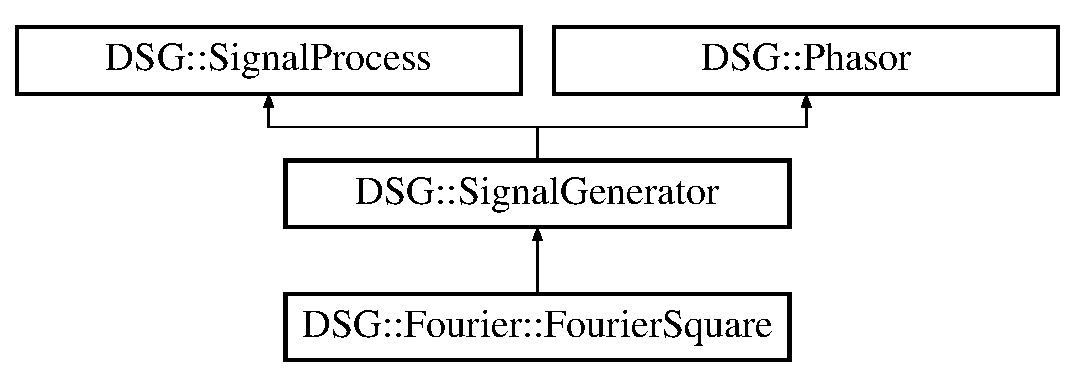
\includegraphics[height=3.000000cm]{class_d_s_g_1_1_fourier_1_1_fourier_square}
\end{center}
\end{figure}
\subsection*{Public Member Functions}
\begin{DoxyCompactItemize}
\item 
\hyperlink{class_d_s_g_1_1_fourier_1_1_fourier_square_a48fa53b8b5ea77013e1bbb2b2467d15e}{Fourier\+Square} ()
\item 
\hyperlink{class_d_s_g_1_1_fourier_1_1_fourier_square_a277316295ca15354a6e507a71cb5f0db}{Fourier\+Square} (\hyperlink{namespace_d_s_g_a4315a061386fa1014fda09b15d3a6973}{D\+S\+G\+::\+D\+S\+G\+Frequency} const \&frequency, \hyperlink{namespace_d_s_g_a44431ce1eb0a7300efdd207bc879e52c}{D\+S\+G\+::\+D\+S\+G\+Phase} const \&offset)
\item 
virtual \hyperlink{class_d_s_g_1_1_fourier_1_1_fourier_square_af78565a799ebfd4be03cc0294dff1f85}{$\sim$\+Fourier\+Square} ()
\item 
virtual bool \hyperlink{class_d_s_g_1_1_fourier_1_1_fourier_square_a05bd0cd3e76ca22e1cede5afb47fbbc4}{Perform} (\hyperlink{namespace_d_s_g_ac39a94cd27ebcd9c1e7502d0c624894a}{D\+S\+G\+::\+D\+S\+G\+Sample} \&signal)
\item 
virtual bool \hyperlink{class_d_s_g_1_1_fourier_1_1_fourier_square_a46028a3615f26876f9c613f983141362}{Perform} (\hyperlink{class_d_s_g_1_1_ring_buffer}{D\+S\+G\+::\+Ring\+Buffer} \&signal)
\item 
virtual \hyperlink{namespace_d_s_g_a4315a061386fa1014fda09b15d3a6973}{D\+S\+G\+::\+D\+S\+G\+Frequency} const \& \hyperlink{class_d_s_g_1_1_fourier_1_1_fourier_square_a120cbb563a518c9412190eaa36cb269f}{Frequency} (\hyperlink{namespace_d_s_g_a4315a061386fa1014fda09b15d3a6973}{D\+S\+G\+::\+D\+S\+G\+Frequency} const \&\hyperlink{class_d_s_g_1_1_fourier_1_1_fourier_square_a5817c7b9b793af6a76278065a67acd9c}{value})
\end{DoxyCompactItemize}
\subsection*{Protected Attributes}
\begin{DoxyCompactItemize}
\item 
unsigned long \hyperlink{class_d_s_g_1_1_fourier_1_1_fourier_square_ac482ccc644bac01f3491503a755b453c}{\+\_\+h}
\item 
const double \hyperlink{class_d_s_g_1_1_fourier_1_1_fourier_square_a974287b077bd7bff2b028dd1af75e3d0}{\+\_\+a}
\item 
double \hyperlink{class_d_s_g_1_1_fourier_1_1_fourier_square_a6e20ab344501c18d79d594ec83f34164}{phs}
\item 
double \hyperlink{class_d_s_g_1_1_fourier_1_1_fourier_square_a5817c7b9b793af6a76278065a67acd9c}{value}
\item 
int \hyperlink{class_d_s_g_1_1_fourier_1_1_fourier_square_ad52c23216a09d1933e5b3289f2d54db2}{i}
\end{DoxyCompactItemize}
\subsection*{Additional Inherited Members}


\subsection{Detailed Description}
\hyperlink{class_d_s_g_1_1_fourier_1_1_fourier_square}{D\+S\+G\+::\+Fourier\+::\+Fourier\+Square} -\/ \hyperlink{namespace_d_s_g_1_1_fourier}{Fourier} Series Square Wave Generator. 

Definition at line \hyperlink{_fourier_square_8h_source_l00034}{34} of file \hyperlink{_fourier_square_8h_source}{Fourier\+Square.\+h}.



\subsection{Constructor \& Destructor Documentation}
\hypertarget{class_d_s_g_1_1_fourier_1_1_fourier_square_a48fa53b8b5ea77013e1bbb2b2467d15e}{\index{D\+S\+G\+::\+Fourier\+::\+Fourier\+Square@{D\+S\+G\+::\+Fourier\+::\+Fourier\+Square}!Fourier\+Square@{Fourier\+Square}}
\index{Fourier\+Square@{Fourier\+Square}!D\+S\+G\+::\+Fourier\+::\+Fourier\+Square@{D\+S\+G\+::\+Fourier\+::\+Fourier\+Square}}
\subsubsection[{Fourier\+Square}]{\setlength{\rightskip}{0pt plus 5cm}D\+S\+G\+::\+Fourier\+::\+Fourier\+Square\+::\+Fourier\+Square (
\begin{DoxyParamCaption}
{}
\end{DoxyParamCaption}
)}}\label{class_d_s_g_1_1_fourier_1_1_fourier_square_a48fa53b8b5ea77013e1bbb2b2467d15e}


Definition at line \hyperlink{_fourier_square_8cpp_source_l00025}{25} of file \hyperlink{_fourier_square_8cpp_source}{Fourier\+Square.\+cpp}.


\begin{DoxyCode}
00025 :\hyperlink{class_d_s_g_1_1_signal_generator}{DSG::SignalGenerator}(),\hyperlink{class_d_s_g_1_1_fourier_1_1_fourier_square_a974287b077bd7bff2b028dd1af75e3d0}{\_a}(3.6/\hyperlink{_p_i_8h_a598a3330b3c21701223ee0ca14316eca}{PI}),\hyperlink{class_d_s_g_1_1_fourier_1_1_fourier_square_a6e20ab344501c18d79d594ec83f34164}{phs}(0),\hyperlink{class_d_s_g_1_1_fourier_1_1_fourier_square_a5817c7b9b793af6a76278065a67acd9c}{value}(0),
      \hyperlink{class_d_s_g_1_1_fourier_1_1_fourier_square_ad52c23216a09d1933e5b3289f2d54db2}{i}(0)\{\}
\end{DoxyCode}
\hypertarget{class_d_s_g_1_1_fourier_1_1_fourier_square_a277316295ca15354a6e507a71cb5f0db}{\index{D\+S\+G\+::\+Fourier\+::\+Fourier\+Square@{D\+S\+G\+::\+Fourier\+::\+Fourier\+Square}!Fourier\+Square@{Fourier\+Square}}
\index{Fourier\+Square@{Fourier\+Square}!D\+S\+G\+::\+Fourier\+::\+Fourier\+Square@{D\+S\+G\+::\+Fourier\+::\+Fourier\+Square}}
\subsubsection[{Fourier\+Square}]{\setlength{\rightskip}{0pt plus 5cm}D\+S\+G\+::\+Fourier\+::\+Fourier\+Square\+::\+Fourier\+Square (
\begin{DoxyParamCaption}
\item[{{\bf D\+S\+G\+::\+D\+S\+G\+Frequency} const \&}]{frequency, }
\item[{{\bf D\+S\+G\+::\+D\+S\+G\+Phase} const \&}]{offset}
\end{DoxyParamCaption}
)}}\label{class_d_s_g_1_1_fourier_1_1_fourier_square_a277316295ca15354a6e507a71cb5f0db}


Definition at line \hyperlink{_fourier_square_8cpp_source_l00026}{26} of file \hyperlink{_fourier_square_8cpp_source}{Fourier\+Square.\+cpp}.


\begin{DoxyCode}
00026                                                                                                 :
      \hyperlink{class_d_s_g_1_1_signal_generator}{DSG::SignalGenerator}(frequency,offset),\hyperlink{class_d_s_g_1_1_fourier_1_1_fourier_square_a974287b077bd7bff2b028dd1af75e3d0}{\_a}(3.6/\hyperlink{_p_i_8h_a598a3330b3c21701223ee0ca14316eca}{PI}),\hyperlink{class_d_s_g_1_1_fourier_1_1_fourier_square_a6e20ab344501c18d79d594ec83f34164}{phs}(0),
      \hyperlink{class_d_s_g_1_1_fourier_1_1_fourier_square_a5817c7b9b793af6a76278065a67acd9c}{value}(0),\hyperlink{class_d_s_g_1_1_fourier_1_1_fourier_square_ad52c23216a09d1933e5b3289f2d54db2}{i}(0)\{
00027     \hyperlink{class_d_s_g_1_1_fourier_1_1_fourier_square_ac482ccc644bac01f3491503a755b453c}{\_h} = \hyperlink{namespace_d_s_g_ab5c4eea42ea10b69cfc32afb83ff1d0d}{MaxHarms}(\hyperlink{class_d_s_g_1_1_signal_generator_a335e7ef058848eca368be51d8544d143}{\_frequency})+1;
00028 \}
\end{DoxyCode}
\hypertarget{class_d_s_g_1_1_fourier_1_1_fourier_square_af78565a799ebfd4be03cc0294dff1f85}{\index{D\+S\+G\+::\+Fourier\+::\+Fourier\+Square@{D\+S\+G\+::\+Fourier\+::\+Fourier\+Square}!````~Fourier\+Square@{$\sim$\+Fourier\+Square}}
\index{````~Fourier\+Square@{$\sim$\+Fourier\+Square}!D\+S\+G\+::\+Fourier\+::\+Fourier\+Square@{D\+S\+G\+::\+Fourier\+::\+Fourier\+Square}}
\subsubsection[{$\sim$\+Fourier\+Square}]{\setlength{\rightskip}{0pt plus 5cm}D\+S\+G\+::\+Fourier\+::\+Fourier\+Square\+::$\sim$\+Fourier\+Square (
\begin{DoxyParamCaption}
{}
\end{DoxyParamCaption}
)\hspace{0.3cm}{\ttfamily [virtual]}}}\label{class_d_s_g_1_1_fourier_1_1_fourier_square_af78565a799ebfd4be03cc0294dff1f85}


Definition at line \hyperlink{_fourier_square_8cpp_source_l00029}{29} of file \hyperlink{_fourier_square_8cpp_source}{Fourier\+Square.\+cpp}.


\begin{DoxyCode}
00029 \{\}\end{DoxyCode}


\subsection{Member Function Documentation}
\hypertarget{class_d_s_g_1_1_fourier_1_1_fourier_square_a120cbb563a518c9412190eaa36cb269f}{\index{D\+S\+G\+::\+Fourier\+::\+Fourier\+Square@{D\+S\+G\+::\+Fourier\+::\+Fourier\+Square}!Frequency@{Frequency}}
\index{Frequency@{Frequency}!D\+S\+G\+::\+Fourier\+::\+Fourier\+Square@{D\+S\+G\+::\+Fourier\+::\+Fourier\+Square}}
\subsubsection[{Frequency}]{\setlength{\rightskip}{0pt plus 5cm}{\bf D\+S\+G\+::\+D\+S\+G\+Frequency} const \& D\+S\+G\+::\+Fourier\+::\+Fourier\+Square\+::\+Frequency (
\begin{DoxyParamCaption}
\item[{{\bf D\+S\+G\+::\+D\+S\+G\+Frequency} const \&}]{value}
\end{DoxyParamCaption}
)\hspace{0.3cm}{\ttfamily [inline]}, {\ttfamily [virtual]}}}\label{class_d_s_g_1_1_fourier_1_1_fourier_square_a120cbb563a518c9412190eaa36cb269f}


Reimplemented from \hyperlink{class_d_s_g_1_1_signal_generator_a30a79888f209d692df3d38f53fc58dfe}{D\+S\+G\+::\+Signal\+Generator}.



Definition at line \hyperlink{_fourier_square_8h_source_l00069}{69} of file \hyperlink{_fourier_square_8h_source}{Fourier\+Square.\+h}.


\begin{DoxyCode}
00069                                                                                                     \{
00070             \hyperlink{class_d_s_g_1_1_signal_generator_a335e7ef058848eca368be51d8544d143}{\_frequency} = \hyperlink{class_d_s_g_1_1_fourier_1_1_fourier_square_a5817c7b9b793af6a76278065a67acd9c}{value};
00071             \hyperlink{class_d_s_g_1_1_signal_generator_a01c046bb52bbb74afd789fdce7978f65}{\_dt} = \hyperlink{class_d_s_g_1_1_signal_generator_a335e7ef058848eca368be51d8544d143}{\_frequency}/\hyperlink{namespace_d_s_g_a72df05177db0412c3590070923f62819}{DSG::SampleRate}();
00072             \hyperlink{class_d_s_g_1_1_fourier_1_1_fourier_square_ac482ccc644bac01f3491503a755b453c}{\_h} = \hyperlink{namespace_d_s_g_ab5c4eea42ea10b69cfc32afb83ff1d0d}{MaxHarms}(\hyperlink{class_d_s_g_1_1_signal_generator_a335e7ef058848eca368be51d8544d143}{\_frequency});
00073             \textcolor{keywordflow}{return} \hyperlink{class_d_s_g_1_1_signal_generator_a335e7ef058848eca368be51d8544d143}{\_frequency};
00074         \}
\end{DoxyCode}
\hypertarget{class_d_s_g_1_1_fourier_1_1_fourier_square_a05bd0cd3e76ca22e1cede5afb47fbbc4}{\index{D\+S\+G\+::\+Fourier\+::\+Fourier\+Square@{D\+S\+G\+::\+Fourier\+::\+Fourier\+Square}!Perform@{Perform}}
\index{Perform@{Perform}!D\+S\+G\+::\+Fourier\+::\+Fourier\+Square@{D\+S\+G\+::\+Fourier\+::\+Fourier\+Square}}
\subsubsection[{Perform}]{\setlength{\rightskip}{0pt plus 5cm}bool D\+S\+G\+::\+Fourier\+::\+Fourier\+Square\+::\+Perform (
\begin{DoxyParamCaption}
\item[{{\bf D\+S\+G\+::\+D\+S\+G\+Sample} \&}]{signal}
\end{DoxyParamCaption}
)\hspace{0.3cm}{\ttfamily [inline]}, {\ttfamily [virtual]}}}\label{class_d_s_g_1_1_fourier_1_1_fourier_square_a05bd0cd3e76ca22e1cede5afb47fbbc4}


Reimplemented from \hyperlink{class_d_s_g_1_1_signal_generator_a46fe75a81a242e191c5049d33ddf4155}{D\+S\+G\+::\+Signal\+Generator}.



Definition at line \hyperlink{_fourier_square_8h_source_l00049}{49} of file \hyperlink{_fourier_square_8h_source}{Fourier\+Square.\+h}.


\begin{DoxyCode}
00049                                                                         \{
00050             \textcolor{comment}{//(\_h/2)+1 Sine Calls Per Sample}
00051             \hyperlink{class_d_s_g_1_1_fourier_1_1_fourier_square_a5817c7b9b793af6a76278065a67acd9c}{value}=\hyperlink{namespace_d_s_g_aad63d316081c7d13a551acf346ee2749}{DSG::Sin}(\hyperlink{class_d_s_g_1_1_signal_generator_a1e23eb94e204b11db75fca030b951065}{\_phasor});\textcolor{comment}{//i=1}
00052             \textcolor{keywordflow}{for} (\hyperlink{class_d_s_g_1_1_fourier_1_1_fourier_square_ad52c23216a09d1933e5b3289f2d54db2}{i}=3; \hyperlink{class_d_s_g_1_1_fourier_1_1_fourier_square_ad52c23216a09d1933e5b3289f2d54db2}{i}<\hyperlink{class_d_s_g_1_1_fourier_1_1_fourier_square_ac482ccc644bac01f3491503a755b453c}{\_h}; \hyperlink{class_d_s_g_1_1_fourier_1_1_fourier_square_ad52c23216a09d1933e5b3289f2d54db2}{i}+=2) \{\textcolor{comment}{//i=3..5..7..}
00053                 \hyperlink{class_d_s_g_1_1_fourier_1_1_fourier_square_a5817c7b9b793af6a76278065a67acd9c}{value} += (1.0/\hyperlink{class_d_s_g_1_1_fourier_1_1_fourier_square_ad52c23216a09d1933e5b3289f2d54db2}{i}) * \hyperlink{namespace_d_s_g_aad63d316081c7d13a551acf346ee2749}{DSG::Sin}(\hyperlink{class_d_s_g_1_1_signal_generator_a1e23eb94e204b11db75fca030b951065}{\_phasor}*\hyperlink{class_d_s_g_1_1_fourier_1_1_fourier_square_ad52c23216a09d1933e5b3289f2d54db2}{i});
00054             \}
00055             \hyperlink{class_d_s_g_1_1_fourier_1_1_fourier_square_a5817c7b9b793af6a76278065a67acd9c}{value}*=\hyperlink{class_d_s_g_1_1_fourier_1_1_fourier_square_a974287b077bd7bff2b028dd1af75e3d0}{\_a};
00056             signal = \hyperlink{class_d_s_g_1_1_fourier_1_1_fourier_square_a5817c7b9b793af6a76278065a67acd9c}{value};
00057             \hyperlink{class_d_s_g_1_1_signal_generator_a4c034c5b9ef3dc7548839288355643d5}{step}();
00058             \textcolor{keywordflow}{return} \textcolor{keyword}{true};
00059         \}
\end{DoxyCode}
\hypertarget{class_d_s_g_1_1_fourier_1_1_fourier_square_a46028a3615f26876f9c613f983141362}{\index{D\+S\+G\+::\+Fourier\+::\+Fourier\+Square@{D\+S\+G\+::\+Fourier\+::\+Fourier\+Square}!Perform@{Perform}}
\index{Perform@{Perform}!D\+S\+G\+::\+Fourier\+::\+Fourier\+Square@{D\+S\+G\+::\+Fourier\+::\+Fourier\+Square}}
\subsubsection[{Perform}]{\setlength{\rightskip}{0pt plus 5cm}bool D\+S\+G\+::\+Fourier\+::\+Fourier\+Square\+::\+Perform (
\begin{DoxyParamCaption}
\item[{{\bf D\+S\+G\+::\+Ring\+Buffer} \&}]{signal}
\end{DoxyParamCaption}
)\hspace{0.3cm}{\ttfamily [inline]}, {\ttfamily [virtual]}}}\label{class_d_s_g_1_1_fourier_1_1_fourier_square_a46028a3615f26876f9c613f983141362}


Reimplemented from \hyperlink{class_d_s_g_1_1_signal_generator_ab050f80e84e6c8b3e354b56930d6a02b}{D\+S\+G\+::\+Signal\+Generator}.



Definition at line \hyperlink{_fourier_square_8h_source_l00060}{60} of file \hyperlink{_fourier_square_8h_source}{Fourier\+Square.\+h}.


\begin{DoxyCode}
00060                                                                          \{
00061             signal.\hyperlink{class_d_s_g_1_1_ring_buffer_ab23c8003d2857809a816068eeb209d60}{Flush}();
00062             \textcolor{keywordflow}{while} (!signal.\hyperlink{class_d_s_g_1_1_ring_buffer_a53ddb04ffcbb5470a8d2b0a3c65b70cb}{Full}()) \{
00063                 \textcolor{keywordflow}{if} (\hyperlink{class_d_s_g_1_1_fourier_1_1_fourier_square_a05bd0cd3e76ca22e1cede5afb47fbbc4}{Perform}(\hyperlink{class_d_s_g_1_1_signal_generator_a28a9b47a1aa0783029f11a19ba0363f2}{\_storage})) \{
00064                     \textcolor{keywordflow}{if}(signal.\hyperlink{class_d_s_g_1_1_ring_buffer_aa5dd2caa0a270173251faee40a43d692}{Write}(\hyperlink{class_d_s_g_1_1_signal_generator_a28a9b47a1aa0783029f11a19ba0363f2}{\_storage}))\{
00065                     \}\textcolor{keywordflow}{else} \textcolor{keywordflow}{return} \textcolor{keyword}{false};
00066                 \}\textcolor{keywordflow}{else} \textcolor{keywordflow}{return} \textcolor{keyword}{false};
00067             \}\textcolor{keywordflow}{return} \textcolor{keyword}{true};
00068         \}
\end{DoxyCode}


\subsection{Member Data Documentation}
\hypertarget{class_d_s_g_1_1_fourier_1_1_fourier_square_a974287b077bd7bff2b028dd1af75e3d0}{\index{D\+S\+G\+::\+Fourier\+::\+Fourier\+Square@{D\+S\+G\+::\+Fourier\+::\+Fourier\+Square}!\+\_\+a@{\+\_\+a}}
\index{\+\_\+a@{\+\_\+a}!D\+S\+G\+::\+Fourier\+::\+Fourier\+Square@{D\+S\+G\+::\+Fourier\+::\+Fourier\+Square}}
\subsubsection[{\+\_\+a}]{\setlength{\rightskip}{0pt plus 5cm}const double D\+S\+G\+::\+Fourier\+::\+Fourier\+Square\+::\+\_\+a\hspace{0.3cm}{\ttfamily [protected]}}}\label{class_d_s_g_1_1_fourier_1_1_fourier_square_a974287b077bd7bff2b028dd1af75e3d0}


Definition at line \hyperlink{_fourier_square_8h_source_l00044}{44} of file \hyperlink{_fourier_square_8h_source}{Fourier\+Square.\+h}.

\hypertarget{class_d_s_g_1_1_fourier_1_1_fourier_square_ac482ccc644bac01f3491503a755b453c}{\index{D\+S\+G\+::\+Fourier\+::\+Fourier\+Square@{D\+S\+G\+::\+Fourier\+::\+Fourier\+Square}!\+\_\+h@{\+\_\+h}}
\index{\+\_\+h@{\+\_\+h}!D\+S\+G\+::\+Fourier\+::\+Fourier\+Square@{D\+S\+G\+::\+Fourier\+::\+Fourier\+Square}}
\subsubsection[{\+\_\+h}]{\setlength{\rightskip}{0pt plus 5cm}unsigned long D\+S\+G\+::\+Fourier\+::\+Fourier\+Square\+::\+\_\+h\hspace{0.3cm}{\ttfamily [protected]}}}\label{class_d_s_g_1_1_fourier_1_1_fourier_square_ac482ccc644bac01f3491503a755b453c}


Definition at line \hyperlink{_fourier_square_8h_source_l00043}{43} of file \hyperlink{_fourier_square_8h_source}{Fourier\+Square.\+h}.

\hypertarget{class_d_s_g_1_1_fourier_1_1_fourier_square_ad52c23216a09d1933e5b3289f2d54db2}{\index{D\+S\+G\+::\+Fourier\+::\+Fourier\+Square@{D\+S\+G\+::\+Fourier\+::\+Fourier\+Square}!i@{i}}
\index{i@{i}!D\+S\+G\+::\+Fourier\+::\+Fourier\+Square@{D\+S\+G\+::\+Fourier\+::\+Fourier\+Square}}
\subsubsection[{i}]{\setlength{\rightskip}{0pt plus 5cm}int D\+S\+G\+::\+Fourier\+::\+Fourier\+Square\+::i\hspace{0.3cm}{\ttfamily [protected]}}}\label{class_d_s_g_1_1_fourier_1_1_fourier_square_ad52c23216a09d1933e5b3289f2d54db2}


Definition at line \hyperlink{_fourier_square_8h_source_l00047}{47} of file \hyperlink{_fourier_square_8h_source}{Fourier\+Square.\+h}.

\hypertarget{class_d_s_g_1_1_fourier_1_1_fourier_square_a6e20ab344501c18d79d594ec83f34164}{\index{D\+S\+G\+::\+Fourier\+::\+Fourier\+Square@{D\+S\+G\+::\+Fourier\+::\+Fourier\+Square}!phs@{phs}}
\index{phs@{phs}!D\+S\+G\+::\+Fourier\+::\+Fourier\+Square@{D\+S\+G\+::\+Fourier\+::\+Fourier\+Square}}
\subsubsection[{phs}]{\setlength{\rightskip}{0pt plus 5cm}double D\+S\+G\+::\+Fourier\+::\+Fourier\+Square\+::phs\hspace{0.3cm}{\ttfamily [protected]}}}\label{class_d_s_g_1_1_fourier_1_1_fourier_square_a6e20ab344501c18d79d594ec83f34164}


Definition at line \hyperlink{_fourier_square_8h_source_l00045}{45} of file \hyperlink{_fourier_square_8h_source}{Fourier\+Square.\+h}.

\hypertarget{class_d_s_g_1_1_fourier_1_1_fourier_square_a5817c7b9b793af6a76278065a67acd9c}{\index{D\+S\+G\+::\+Fourier\+::\+Fourier\+Square@{D\+S\+G\+::\+Fourier\+::\+Fourier\+Square}!value@{value}}
\index{value@{value}!D\+S\+G\+::\+Fourier\+::\+Fourier\+Square@{D\+S\+G\+::\+Fourier\+::\+Fourier\+Square}}
\subsubsection[{value}]{\setlength{\rightskip}{0pt plus 5cm}double D\+S\+G\+::\+Fourier\+::\+Fourier\+Square\+::value\hspace{0.3cm}{\ttfamily [protected]}}}\label{class_d_s_g_1_1_fourier_1_1_fourier_square_a5817c7b9b793af6a76278065a67acd9c}


Definition at line \hyperlink{_fourier_square_8h_source_l00046}{46} of file \hyperlink{_fourier_square_8h_source}{Fourier\+Square.\+h}.



The documentation for this class was generated from the following files\+:\begin{DoxyCompactItemize}
\item 
\hyperlink{_fourier_square_8h}{Fourier\+Square.\+h}\item 
\hyperlink{_fourier_square_8cpp}{Fourier\+Square.\+cpp}\end{DoxyCompactItemize}

\hypertarget{class_d_s_g_1_1_fourier_1_1_fourier_triangle}{\section{D\+S\+G\+:\+:Fourier\+:\+:Fourier\+Triangle Class Reference}
\label{class_d_s_g_1_1_fourier_1_1_fourier_triangle}\index{D\+S\+G\+::\+Fourier\+::\+Fourier\+Triangle@{D\+S\+G\+::\+Fourier\+::\+Fourier\+Triangle}}
}


\hyperlink{class_d_s_g_1_1_fourier_1_1_fourier_triangle}{D\+S\+G\+::\+Fourier\+::\+Fourier\+Triangle} -\/ \hyperlink{namespace_d_s_g_1_1_fourier}{Fourier} Series Triangle Wave Generator.  




{\ttfamily \#include $<$Fourier\+Triangle.\+h$>$}

Inheritance diagram for D\+S\+G\+:\+:Fourier\+:\+:Fourier\+Triangle\+:\begin{figure}[H]
\begin{center}
\leavevmode
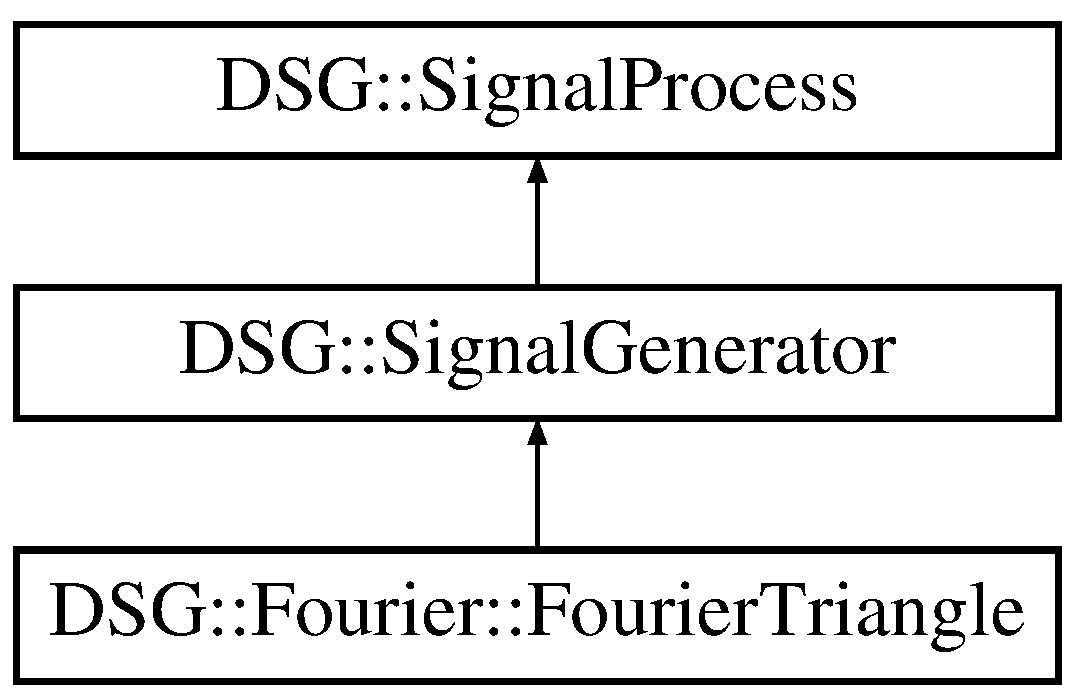
\includegraphics[height=3.000000cm]{class_d_s_g_1_1_fourier_1_1_fourier_triangle}
\end{center}
\end{figure}
\subsection*{Public Member Functions}
\begin{DoxyCompactItemize}
\item 
\hyperlink{class_d_s_g_1_1_fourier_1_1_fourier_triangle_a4129c053eddd87256ae39552a06ce329}{Fourier\+Triangle} ()
\item 
\hyperlink{class_d_s_g_1_1_fourier_1_1_fourier_triangle_abf887c6f5aada92780224511988cb688}{Fourier\+Triangle} (\hyperlink{namespace_d_s_g_a4315a061386fa1014fda09b15d3a6973}{D\+S\+G\+::\+D\+S\+G\+Frequency} const \&frequency, \hyperlink{namespace_d_s_g_a44431ce1eb0a7300efdd207bc879e52c}{D\+S\+G\+::\+D\+S\+G\+Phase} const \&offset)
\item 
virtual \hyperlink{class_d_s_g_1_1_fourier_1_1_fourier_triangle_a780bfb898d144200ff2bfb48849b4d24}{$\sim$\+Fourier\+Triangle} ()
\item 
virtual bool \hyperlink{class_d_s_g_1_1_fourier_1_1_fourier_triangle_ab5b947c1fc1f34a461c863b18e3e877d}{Perform} (\hyperlink{namespace_d_s_g_ac39a94cd27ebcd9c1e7502d0c624894a}{D\+S\+G\+::\+D\+S\+G\+Sample} \&signal)
\item 
virtual bool \hyperlink{class_d_s_g_1_1_fourier_1_1_fourier_triangle_a27b082e69cc7d70223dd3fbc552ba5bc}{Perform} (\hyperlink{class_d_s_g_1_1_ring_buffer}{D\+S\+G\+::\+Ring\+Buffer} \&signal)
\item 
virtual \hyperlink{namespace_d_s_g_a4315a061386fa1014fda09b15d3a6973}{D\+S\+G\+::\+D\+S\+G\+Frequency} const \& \hyperlink{class_d_s_g_1_1_fourier_1_1_fourier_triangle_a278a51ed8af32ea371adc903b9b25039}{Frequency} (\hyperlink{namespace_d_s_g_a4315a061386fa1014fda09b15d3a6973}{D\+S\+G\+::\+D\+S\+G\+Frequency} const \&\hyperlink{class_d_s_g_1_1_fourier_1_1_fourier_triangle_a11216186ce96fc78c7720cad3e01d025}{value})
\end{DoxyCompactItemize}
\subsection*{Protected Attributes}
\begin{DoxyCompactItemize}
\item 
unsigned long \hyperlink{class_d_s_g_1_1_fourier_1_1_fourier_triangle_a6fe21fae0d58d6221602e4bd74c30a80}{\+\_\+h}
\item 
const double \hyperlink{class_d_s_g_1_1_fourier_1_1_fourier_triangle_a64263fc3fa98179d57d34a3f105d8c97}{\+\_\+a}
\item 
double \hyperlink{class_d_s_g_1_1_fourier_1_1_fourier_triangle_a274fb09e2f14f88ec969dcaa7ad423f4}{phs}
\item 
double \hyperlink{class_d_s_g_1_1_fourier_1_1_fourier_triangle_a11216186ce96fc78c7720cad3e01d025}{value}
\item 
int \hyperlink{class_d_s_g_1_1_fourier_1_1_fourier_triangle_a041154af261bce33f4764f60b6606ea4}{i}
\end{DoxyCompactItemize}
\subsection*{Additional Inherited Members}


\subsection{Detailed Description}
\hyperlink{class_d_s_g_1_1_fourier_1_1_fourier_triangle}{D\+S\+G\+::\+Fourier\+::\+Fourier\+Triangle} -\/ \hyperlink{namespace_d_s_g_1_1_fourier}{Fourier} Series Triangle Wave Generator. 

Definition at line \hyperlink{_fourier_triangle_8h_source_l00034}{34} of file \hyperlink{_fourier_triangle_8h_source}{Fourier\+Triangle.\+h}.



\subsection{Constructor \& Destructor Documentation}
\hypertarget{class_d_s_g_1_1_fourier_1_1_fourier_triangle_a4129c053eddd87256ae39552a06ce329}{\index{D\+S\+G\+::\+Fourier\+::\+Fourier\+Triangle@{D\+S\+G\+::\+Fourier\+::\+Fourier\+Triangle}!Fourier\+Triangle@{Fourier\+Triangle}}
\index{Fourier\+Triangle@{Fourier\+Triangle}!D\+S\+G\+::\+Fourier\+::\+Fourier\+Triangle@{D\+S\+G\+::\+Fourier\+::\+Fourier\+Triangle}}
\subsubsection[{Fourier\+Triangle}]{\setlength{\rightskip}{0pt plus 5cm}D\+S\+G\+::\+Fourier\+::\+Fourier\+Triangle\+::\+Fourier\+Triangle (
\begin{DoxyParamCaption}
{}
\end{DoxyParamCaption}
)}}\label{class_d_s_g_1_1_fourier_1_1_fourier_triangle_a4129c053eddd87256ae39552a06ce329}


Definition at line \hyperlink{_fourier_triangle_8cpp_source_l00025}{25} of file \hyperlink{_fourier_triangle_8cpp_source}{Fourier\+Triangle.\+cpp}.


\begin{DoxyCode}
00025 :\hyperlink{class_d_s_g_1_1_signal_generator}{DSG::SignalGenerator}(),\hyperlink{class_d_s_g_1_1_fourier_1_1_fourier_triangle_a64263fc3fa98179d57d34a3f105d8c97}{\_a}(8.0/(\hyperlink{_p_i_8h_a598a3330b3c21701223ee0ca14316eca}{PI}*\hyperlink{_p_i_8h_a598a3330b3c21701223ee0ca14316eca}{PI})),\hyperlink{class_d_s_g_1_1_fourier_1_1_fourier_triangle_a274fb09e2f14f88ec969dcaa7ad423f4}{phs}(0),
      \hyperlink{class_d_s_g_1_1_fourier_1_1_fourier_triangle_a11216186ce96fc78c7720cad3e01d025}{value}(0),\hyperlink{class_d_s_g_1_1_fourier_1_1_fourier_triangle_a041154af261bce33f4764f60b6606ea4}{i}(0)\{\}
\end{DoxyCode}
\hypertarget{class_d_s_g_1_1_fourier_1_1_fourier_triangle_abf887c6f5aada92780224511988cb688}{\index{D\+S\+G\+::\+Fourier\+::\+Fourier\+Triangle@{D\+S\+G\+::\+Fourier\+::\+Fourier\+Triangle}!Fourier\+Triangle@{Fourier\+Triangle}}
\index{Fourier\+Triangle@{Fourier\+Triangle}!D\+S\+G\+::\+Fourier\+::\+Fourier\+Triangle@{D\+S\+G\+::\+Fourier\+::\+Fourier\+Triangle}}
\subsubsection[{Fourier\+Triangle}]{\setlength{\rightskip}{0pt plus 5cm}D\+S\+G\+::\+Fourier\+::\+Fourier\+Triangle\+::\+Fourier\+Triangle (
\begin{DoxyParamCaption}
\item[{{\bf D\+S\+G\+::\+D\+S\+G\+Frequency} const \&}]{frequency, }
\item[{{\bf D\+S\+G\+::\+D\+S\+G\+Phase} const \&}]{offset}
\end{DoxyParamCaption}
)}}\label{class_d_s_g_1_1_fourier_1_1_fourier_triangle_abf887c6f5aada92780224511988cb688}


Definition at line \hyperlink{_fourier_triangle_8cpp_source_l00026}{26} of file \hyperlink{_fourier_triangle_8cpp_source}{Fourier\+Triangle.\+cpp}.


\begin{DoxyCode}
00026                                                                                                     :
      \hyperlink{class_d_s_g_1_1_signal_generator}{DSG::SignalGenerator}(frequency,offset),\hyperlink{class_d_s_g_1_1_fourier_1_1_fourier_triangle_a64263fc3fa98179d57d34a3f105d8c97}{\_a}(8.0/(\hyperlink{_p_i_8h_a598a3330b3c21701223ee0ca14316eca}{PI}*\hyperlink{_p_i_8h_a598a3330b3c21701223ee0ca14316eca}{PI})),
      \hyperlink{class_d_s_g_1_1_fourier_1_1_fourier_triangle_a274fb09e2f14f88ec969dcaa7ad423f4}{phs}(0),\hyperlink{class_d_s_g_1_1_fourier_1_1_fourier_triangle_a11216186ce96fc78c7720cad3e01d025}{value}(0),\hyperlink{class_d_s_g_1_1_fourier_1_1_fourier_triangle_a041154af261bce33f4764f60b6606ea4}{i}(0)\{
00027     \hyperlink{class_d_s_g_1_1_fourier_1_1_fourier_triangle_a6fe21fae0d58d6221602e4bd74c30a80}{\_h} = \hyperlink{namespace_d_s_g_ab5c4eea42ea10b69cfc32afb83ff1d0d}{MaxHarms}(\hyperlink{class_d_s_g_1_1_signal_generator_a335e7ef058848eca368be51d8544d143}{\_frequency})+1;
00028 \}
\end{DoxyCode}
\hypertarget{class_d_s_g_1_1_fourier_1_1_fourier_triangle_a780bfb898d144200ff2bfb48849b4d24}{\index{D\+S\+G\+::\+Fourier\+::\+Fourier\+Triangle@{D\+S\+G\+::\+Fourier\+::\+Fourier\+Triangle}!````~Fourier\+Triangle@{$\sim$\+Fourier\+Triangle}}
\index{````~Fourier\+Triangle@{$\sim$\+Fourier\+Triangle}!D\+S\+G\+::\+Fourier\+::\+Fourier\+Triangle@{D\+S\+G\+::\+Fourier\+::\+Fourier\+Triangle}}
\subsubsection[{$\sim$\+Fourier\+Triangle}]{\setlength{\rightskip}{0pt plus 5cm}D\+S\+G\+::\+Fourier\+::\+Fourier\+Triangle\+::$\sim$\+Fourier\+Triangle (
\begin{DoxyParamCaption}
{}
\end{DoxyParamCaption}
)\hspace{0.3cm}{\ttfamily [virtual]}}}\label{class_d_s_g_1_1_fourier_1_1_fourier_triangle_a780bfb898d144200ff2bfb48849b4d24}


Definition at line \hyperlink{_fourier_triangle_8cpp_source_l00029}{29} of file \hyperlink{_fourier_triangle_8cpp_source}{Fourier\+Triangle.\+cpp}.


\begin{DoxyCode}
00029 \{\}\end{DoxyCode}


\subsection{Member Function Documentation}
\hypertarget{class_d_s_g_1_1_fourier_1_1_fourier_triangle_a278a51ed8af32ea371adc903b9b25039}{\index{D\+S\+G\+::\+Fourier\+::\+Fourier\+Triangle@{D\+S\+G\+::\+Fourier\+::\+Fourier\+Triangle}!Frequency@{Frequency}}
\index{Frequency@{Frequency}!D\+S\+G\+::\+Fourier\+::\+Fourier\+Triangle@{D\+S\+G\+::\+Fourier\+::\+Fourier\+Triangle}}
\subsubsection[{Frequency}]{\setlength{\rightskip}{0pt plus 5cm}{\bf D\+S\+G\+::\+D\+S\+G\+Frequency} const \& D\+S\+G\+::\+Fourier\+::\+Fourier\+Triangle\+::\+Frequency (
\begin{DoxyParamCaption}
\item[{{\bf D\+S\+G\+::\+D\+S\+G\+Frequency} const \&}]{value}
\end{DoxyParamCaption}
)\hspace{0.3cm}{\ttfamily [inline]}, {\ttfamily [virtual]}}}\label{class_d_s_g_1_1_fourier_1_1_fourier_triangle_a278a51ed8af32ea371adc903b9b25039}


Reimplemented from \hyperlink{class_d_s_g_1_1_signal_generator_a30a79888f209d692df3d38f53fc58dfe}{D\+S\+G\+::\+Signal\+Generator}.



Definition at line \hyperlink{_fourier_triangle_8h_source_l00071}{71} of file \hyperlink{_fourier_triangle_8h_source}{Fourier\+Triangle.\+h}.


\begin{DoxyCode}
00071                                                                                                       \{
00072             \hyperlink{class_d_s_g_1_1_signal_generator_a335e7ef058848eca368be51d8544d143}{\_frequency} = \hyperlink{class_d_s_g_1_1_fourier_1_1_fourier_triangle_a11216186ce96fc78c7720cad3e01d025}{value};
00073             \hyperlink{class_d_s_g_1_1_signal_generator_a01c046bb52bbb74afd789fdce7978f65}{\_dt} = \hyperlink{class_d_s_g_1_1_signal_generator_a335e7ef058848eca368be51d8544d143}{\_frequency}/\hyperlink{namespace_d_s_g_a72df05177db0412c3590070923f62819}{DSG::SampleRate}();
00074             \hyperlink{class_d_s_g_1_1_fourier_1_1_fourier_triangle_a6fe21fae0d58d6221602e4bd74c30a80}{\_h} = \hyperlink{namespace_d_s_g_ab5c4eea42ea10b69cfc32afb83ff1d0d}{MaxHarms}(\hyperlink{class_d_s_g_1_1_signal_generator_a335e7ef058848eca368be51d8544d143}{\_frequency});
00075             \textcolor{keywordflow}{return} \hyperlink{class_d_s_g_1_1_signal_generator_a335e7ef058848eca368be51d8544d143}{\_frequency};
00076         \}
\end{DoxyCode}
\hypertarget{class_d_s_g_1_1_fourier_1_1_fourier_triangle_ab5b947c1fc1f34a461c863b18e3e877d}{\index{D\+S\+G\+::\+Fourier\+::\+Fourier\+Triangle@{D\+S\+G\+::\+Fourier\+::\+Fourier\+Triangle}!Perform@{Perform}}
\index{Perform@{Perform}!D\+S\+G\+::\+Fourier\+::\+Fourier\+Triangle@{D\+S\+G\+::\+Fourier\+::\+Fourier\+Triangle}}
\subsubsection[{Perform}]{\setlength{\rightskip}{0pt plus 5cm}bool D\+S\+G\+::\+Fourier\+::\+Fourier\+Triangle\+::\+Perform (
\begin{DoxyParamCaption}
\item[{{\bf D\+S\+G\+::\+D\+S\+G\+Sample} \&}]{signal}
\end{DoxyParamCaption}
)\hspace{0.3cm}{\ttfamily [inline]}, {\ttfamily [virtual]}}}\label{class_d_s_g_1_1_fourier_1_1_fourier_triangle_ab5b947c1fc1f34a461c863b18e3e877d}


Reimplemented from \hyperlink{class_d_s_g_1_1_signal_generator_a46fe75a81a242e191c5049d33ddf4155}{D\+S\+G\+::\+Signal\+Generator}.



Definition at line \hyperlink{_fourier_triangle_8h_source_l00049}{49} of file \hyperlink{_fourier_triangle_8h_source}{Fourier\+Triangle.\+h}.


\begin{DoxyCode}
00049                                                                           \{
00050             \textcolor{comment}{//(\_h/2)+1 Sine Calls Per Sample}
00051             \hyperlink{class_d_s_g_1_1_fourier_1_1_fourier_triangle_a11216186ce96fc78c7720cad3e01d025}{value}=\hyperlink{namespace_d_s_g_aad63d316081c7d13a551acf346ee2749}{DSG::Sin}(\hyperlink{class_d_s_g_1_1_signal_generator_a1e23eb94e204b11db75fca030b951065}{\_phasor});\textcolor{comment}{//i=1}
00052             \textcolor{keywordtype}{double} sgn = -1;
00053             \textcolor{keywordflow}{for} (\hyperlink{class_d_s_g_1_1_fourier_1_1_fourier_triangle_a041154af261bce33f4764f60b6606ea4}{i}=3; \hyperlink{class_d_s_g_1_1_fourier_1_1_fourier_triangle_a041154af261bce33f4764f60b6606ea4}{i}<\hyperlink{class_d_s_g_1_1_fourier_1_1_fourier_triangle_a6fe21fae0d58d6221602e4bd74c30a80}{\_h}; \hyperlink{class_d_s_g_1_1_fourier_1_1_fourier_triangle_a041154af261bce33f4764f60b6606ea4}{i}+=2) \{\textcolor{comment}{//i=3..5..7..}
00054                 \hyperlink{class_d_s_g_1_1_fourier_1_1_fourier_triangle_a11216186ce96fc78c7720cad3e01d025}{value} += sgn * (1.0/(\hyperlink{class_d_s_g_1_1_fourier_1_1_fourier_triangle_a041154af261bce33f4764f60b6606ea4}{i}*\hyperlink{class_d_s_g_1_1_fourier_1_1_fourier_triangle_a041154af261bce33f4764f60b6606ea4}{i})) * \hyperlink{namespace_d_s_g_aad63d316081c7d13a551acf346ee2749}{DSG::Sin}(\hyperlink{class_d_s_g_1_1_signal_generator_a1e23eb94e204b11db75fca030b951065}{\_phasor}*
      \hyperlink{class_d_s_g_1_1_fourier_1_1_fourier_triangle_a041154af261bce33f4764f60b6606ea4}{i});
00055                 sgn*=-1;
00056             \}
00057             \hyperlink{class_d_s_g_1_1_fourier_1_1_fourier_triangle_a11216186ce96fc78c7720cad3e01d025}{value}*=\hyperlink{class_d_s_g_1_1_fourier_1_1_fourier_triangle_a64263fc3fa98179d57d34a3f105d8c97}{\_a};
00058             signal = \hyperlink{class_d_s_g_1_1_fourier_1_1_fourier_triangle_a11216186ce96fc78c7720cad3e01d025}{value};
00059             \hyperlink{class_d_s_g_1_1_signal_generator_a4c034c5b9ef3dc7548839288355643d5}{step}();
00060             \textcolor{keywordflow}{return} \textcolor{keyword}{true};
00061         \}
\end{DoxyCode}
\hypertarget{class_d_s_g_1_1_fourier_1_1_fourier_triangle_a27b082e69cc7d70223dd3fbc552ba5bc}{\index{D\+S\+G\+::\+Fourier\+::\+Fourier\+Triangle@{D\+S\+G\+::\+Fourier\+::\+Fourier\+Triangle}!Perform@{Perform}}
\index{Perform@{Perform}!D\+S\+G\+::\+Fourier\+::\+Fourier\+Triangle@{D\+S\+G\+::\+Fourier\+::\+Fourier\+Triangle}}
\subsubsection[{Perform}]{\setlength{\rightskip}{0pt plus 5cm}bool D\+S\+G\+::\+Fourier\+::\+Fourier\+Triangle\+::\+Perform (
\begin{DoxyParamCaption}
\item[{{\bf D\+S\+G\+::\+Ring\+Buffer} \&}]{signal}
\end{DoxyParamCaption}
)\hspace{0.3cm}{\ttfamily [inline]}, {\ttfamily [virtual]}}}\label{class_d_s_g_1_1_fourier_1_1_fourier_triangle_a27b082e69cc7d70223dd3fbc552ba5bc}


Reimplemented from \hyperlink{class_d_s_g_1_1_signal_generator_ab050f80e84e6c8b3e354b56930d6a02b}{D\+S\+G\+::\+Signal\+Generator}.



Definition at line \hyperlink{_fourier_triangle_8h_source_l00062}{62} of file \hyperlink{_fourier_triangle_8h_source}{Fourier\+Triangle.\+h}.


\begin{DoxyCode}
00062                                                                            \{
00063             signal.\hyperlink{class_d_s_g_1_1_ring_buffer_ab23c8003d2857809a816068eeb209d60}{Flush}();
00064             \textcolor{keywordflow}{while} (!signal.\hyperlink{class_d_s_g_1_1_ring_buffer_a53ddb04ffcbb5470a8d2b0a3c65b70cb}{Full}()) \{
00065                 \textcolor{keywordflow}{if} (\hyperlink{class_d_s_g_1_1_fourier_1_1_fourier_triangle_ab5b947c1fc1f34a461c863b18e3e877d}{Perform}(\hyperlink{class_d_s_g_1_1_signal_generator_a28a9b47a1aa0783029f11a19ba0363f2}{\_storage})) \{
00066                     \textcolor{keywordflow}{if}(signal.\hyperlink{class_d_s_g_1_1_ring_buffer_aa5dd2caa0a270173251faee40a43d692}{Write}(\hyperlink{class_d_s_g_1_1_signal_generator_a28a9b47a1aa0783029f11a19ba0363f2}{\_storage}))\{
00067                     \}\textcolor{keywordflow}{else} \textcolor{keywordflow}{return} \textcolor{keyword}{false};
00068                 \}\textcolor{keywordflow}{else} \textcolor{keywordflow}{return} \textcolor{keyword}{false};
00069             \}\textcolor{keywordflow}{return} \textcolor{keyword}{true};
00070         \}
\end{DoxyCode}


\subsection{Member Data Documentation}
\hypertarget{class_d_s_g_1_1_fourier_1_1_fourier_triangle_a64263fc3fa98179d57d34a3f105d8c97}{\index{D\+S\+G\+::\+Fourier\+::\+Fourier\+Triangle@{D\+S\+G\+::\+Fourier\+::\+Fourier\+Triangle}!\+\_\+a@{\+\_\+a}}
\index{\+\_\+a@{\+\_\+a}!D\+S\+G\+::\+Fourier\+::\+Fourier\+Triangle@{D\+S\+G\+::\+Fourier\+::\+Fourier\+Triangle}}
\subsubsection[{\+\_\+a}]{\setlength{\rightskip}{0pt plus 5cm}const double D\+S\+G\+::\+Fourier\+::\+Fourier\+Triangle\+::\+\_\+a\hspace{0.3cm}{\ttfamily [protected]}}}\label{class_d_s_g_1_1_fourier_1_1_fourier_triangle_a64263fc3fa98179d57d34a3f105d8c97}


Definition at line \hyperlink{_fourier_triangle_8h_source_l00044}{44} of file \hyperlink{_fourier_triangle_8h_source}{Fourier\+Triangle.\+h}.

\hypertarget{class_d_s_g_1_1_fourier_1_1_fourier_triangle_a6fe21fae0d58d6221602e4bd74c30a80}{\index{D\+S\+G\+::\+Fourier\+::\+Fourier\+Triangle@{D\+S\+G\+::\+Fourier\+::\+Fourier\+Triangle}!\+\_\+h@{\+\_\+h}}
\index{\+\_\+h@{\+\_\+h}!D\+S\+G\+::\+Fourier\+::\+Fourier\+Triangle@{D\+S\+G\+::\+Fourier\+::\+Fourier\+Triangle}}
\subsubsection[{\+\_\+h}]{\setlength{\rightskip}{0pt plus 5cm}unsigned long D\+S\+G\+::\+Fourier\+::\+Fourier\+Triangle\+::\+\_\+h\hspace{0.3cm}{\ttfamily [protected]}}}\label{class_d_s_g_1_1_fourier_1_1_fourier_triangle_a6fe21fae0d58d6221602e4bd74c30a80}


Definition at line \hyperlink{_fourier_triangle_8h_source_l00043}{43} of file \hyperlink{_fourier_triangle_8h_source}{Fourier\+Triangle.\+h}.

\hypertarget{class_d_s_g_1_1_fourier_1_1_fourier_triangle_a041154af261bce33f4764f60b6606ea4}{\index{D\+S\+G\+::\+Fourier\+::\+Fourier\+Triangle@{D\+S\+G\+::\+Fourier\+::\+Fourier\+Triangle}!i@{i}}
\index{i@{i}!D\+S\+G\+::\+Fourier\+::\+Fourier\+Triangle@{D\+S\+G\+::\+Fourier\+::\+Fourier\+Triangle}}
\subsubsection[{i}]{\setlength{\rightskip}{0pt plus 5cm}int D\+S\+G\+::\+Fourier\+::\+Fourier\+Triangle\+::i\hspace{0.3cm}{\ttfamily [protected]}}}\label{class_d_s_g_1_1_fourier_1_1_fourier_triangle_a041154af261bce33f4764f60b6606ea4}


Definition at line \hyperlink{_fourier_triangle_8h_source_l00047}{47} of file \hyperlink{_fourier_triangle_8h_source}{Fourier\+Triangle.\+h}.

\hypertarget{class_d_s_g_1_1_fourier_1_1_fourier_triangle_a274fb09e2f14f88ec969dcaa7ad423f4}{\index{D\+S\+G\+::\+Fourier\+::\+Fourier\+Triangle@{D\+S\+G\+::\+Fourier\+::\+Fourier\+Triangle}!phs@{phs}}
\index{phs@{phs}!D\+S\+G\+::\+Fourier\+::\+Fourier\+Triangle@{D\+S\+G\+::\+Fourier\+::\+Fourier\+Triangle}}
\subsubsection[{phs}]{\setlength{\rightskip}{0pt plus 5cm}double D\+S\+G\+::\+Fourier\+::\+Fourier\+Triangle\+::phs\hspace{0.3cm}{\ttfamily [protected]}}}\label{class_d_s_g_1_1_fourier_1_1_fourier_triangle_a274fb09e2f14f88ec969dcaa7ad423f4}


Definition at line \hyperlink{_fourier_triangle_8h_source_l00045}{45} of file \hyperlink{_fourier_triangle_8h_source}{Fourier\+Triangle.\+h}.

\hypertarget{class_d_s_g_1_1_fourier_1_1_fourier_triangle_a11216186ce96fc78c7720cad3e01d025}{\index{D\+S\+G\+::\+Fourier\+::\+Fourier\+Triangle@{D\+S\+G\+::\+Fourier\+::\+Fourier\+Triangle}!value@{value}}
\index{value@{value}!D\+S\+G\+::\+Fourier\+::\+Fourier\+Triangle@{D\+S\+G\+::\+Fourier\+::\+Fourier\+Triangle}}
\subsubsection[{value}]{\setlength{\rightskip}{0pt plus 5cm}double D\+S\+G\+::\+Fourier\+::\+Fourier\+Triangle\+::value\hspace{0.3cm}{\ttfamily [protected]}}}\label{class_d_s_g_1_1_fourier_1_1_fourier_triangle_a11216186ce96fc78c7720cad3e01d025}


Definition at line \hyperlink{_fourier_triangle_8h_source_l00046}{46} of file \hyperlink{_fourier_triangle_8h_source}{Fourier\+Triangle.\+h}.



The documentation for this class was generated from the following files\+:\begin{DoxyCompactItemize}
\item 
\hyperlink{_fourier_triangle_8h}{Fourier\+Triangle.\+h}\item 
\hyperlink{_fourier_triangle_8cpp}{Fourier\+Triangle.\+cpp}\end{DoxyCompactItemize}

\hypertarget{class_d_s_g_1_1_l_u_t}{\section{D\+S\+G\+:\+:L\+U\+T$<$ element, size $>$ Class Template Reference}
\label{class_d_s_g_1_1_l_u_t}\index{D\+S\+G\+::\+L\+U\+T$<$ element, size $>$@{D\+S\+G\+::\+L\+U\+T$<$ element, size $>$}}
}
Inheritance diagram for D\+S\+G\+:\+:L\+U\+T$<$ element, size $>$\+:\begin{figure}[H]
\begin{center}
\leavevmode
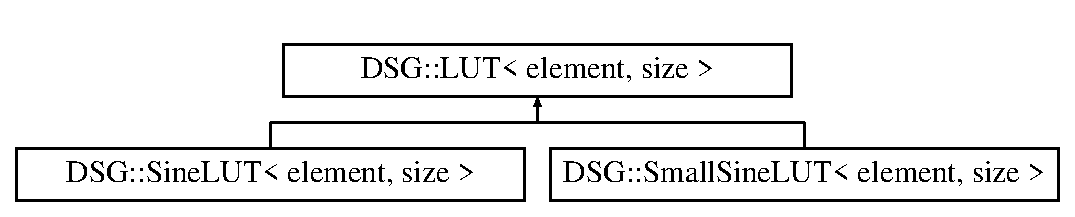
\includegraphics[height=2.000000cm]{class_d_s_g_1_1_l_u_t}
\end{center}
\end{figure}
\subsection*{Public Member Functions}
\begin{DoxyCompactItemize}
\item 
\hypertarget{class_d_s_g_1_1_l_u_t_a5f3bc252bd650fae13046e7959b94f81}{element const \& {\bfseries operator\mbox{[}$\,$\mbox{]}} (unsigned long const \&index)}\label{class_d_s_g_1_1_l_u_t_a5f3bc252bd650fae13046e7959b94f81}

\item 
\hypertarget{class_d_s_g_1_1_l_u_t_a131c3cf974754270699fdcda74f2e694}{virtual element const \& {\bfseries operator()} (double const \&x)}\label{class_d_s_g_1_1_l_u_t_a131c3cf974754270699fdcda74f2e694}

\item 
\hypertarget{class_d_s_g_1_1_l_u_t_a2d1a2112f9e960c7b70882a19d670ff9}{unsigned long const \& {\bfseries Size} () const }\label{class_d_s_g_1_1_l_u_t_a2d1a2112f9e960c7b70882a19d670ff9}

\end{DoxyCompactItemize}
\subsection*{Protected Attributes}
\begin{DoxyCompactItemize}
\item 
\hypertarget{class_d_s_g_1_1_l_u_t_ac8b23bbb7ce259d4ceb1c6fa93a7f29f}{element {\bfseries \+\_\+table} \mbox{[}size\mbox{]}}\label{class_d_s_g_1_1_l_u_t_ac8b23bbb7ce259d4ceb1c6fa93a7f29f}

\item 
\hypertarget{class_d_s_g_1_1_l_u_t_a87c352b5eaea2188955213c0f4ae9799}{const unsigned long {\bfseries \+\_\+size}}\label{class_d_s_g_1_1_l_u_t_a87c352b5eaea2188955213c0f4ae9799}

\end{DoxyCompactItemize}


The documentation for this class was generated from the following file\+:\begin{DoxyCompactItemize}
\item 
/\+Users/alexanderzywicki/\+Documents/\+D\+S\+G/src/L\+U\+T.\+h\end{DoxyCompactItemize}

\hypertarget{class_d_s_g_1_1_ring_buffer}{\section{D\+S\+G\+:\+:Ring\+Buffer Class Reference}
\label{class_d_s_g_1_1_ring_buffer}\index{D\+S\+G\+::\+Ring\+Buffer@{D\+S\+G\+::\+Ring\+Buffer}}
}


\hyperlink{class_d_s_g_1_1_ring_buffer}{D\+S\+G\+::\+Ring\+Buffer} -\/ Circular \hyperlink{class_d_s_g_1_1_buffer}{Buffer} of Audio.  




{\ttfamily \#include $<$Ring\+Buffer.\+h$>$}

Inheritance diagram for D\+S\+G\+:\+:Ring\+Buffer\+:\begin{figure}[H]
\begin{center}
\leavevmode
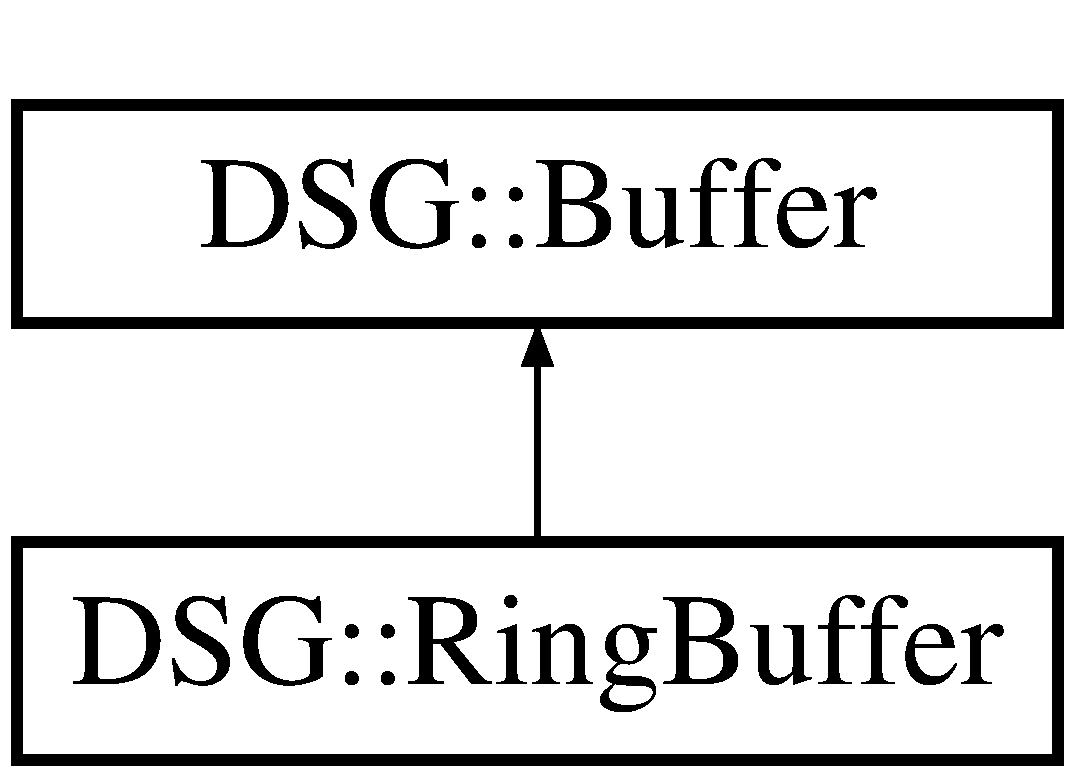
\includegraphics[height=2.000000cm]{class_d_s_g_1_1_ring_buffer}
\end{center}
\end{figure}
\subsection*{Public Member Functions}
\begin{DoxyCompactItemize}
\item 
\hyperlink{class_d_s_g_1_1_ring_buffer_a3136c9debb3c422adb1d5835e11b2b99}{Ring\+Buffer} ()
\item 
\hyperlink{class_d_s_g_1_1_ring_buffer_ae9859fd3ad18961de494d8b50fe4763e}{Ring\+Buffer} (const size\+\_\+t size)
\item 
\hyperlink{class_d_s_g_1_1_ring_buffer_ab09f32dacee49df3281c6701b7a4d737}{Ring\+Buffer} (\hyperlink{class_d_s_g_1_1_ring_buffer}{Ring\+Buffer} \&buffer)
\item 
\hyperlink{class_d_s_g_1_1_ring_buffer}{Ring\+Buffer} \& \hyperlink{class_d_s_g_1_1_ring_buffer_a892fbcc12b2dca5b04ead96a09299e73}{operator=} (\hyperlink{class_d_s_g_1_1_ring_buffer}{Ring\+Buffer} \&buffer)
\item 
virtual \hyperlink{class_d_s_g_1_1_ring_buffer_a771d30b04b6f0313c203530685fbeb3a}{$\sim$\+Ring\+Buffer} ()
\item 
bool \hyperlink{class_d_s_g_1_1_ring_buffer_aa5dd2caa0a270173251faee40a43d692}{Write} (const \hyperlink{namespace_d_s_g_ac39a94cd27ebcd9c1e7502d0c624894a}{D\+S\+G\+Sample} \&elem)
\item 
bool \hyperlink{class_d_s_g_1_1_ring_buffer_a6b2848a64f15c7b0c320779582fa0fbe}{Read} (\hyperlink{namespace_d_s_g_ac39a94cd27ebcd9c1e7502d0c624894a}{D\+S\+G\+::\+D\+S\+G\+Sample} \&elem)
\item 
size\+\_\+t const \& \hyperlink{class_d_s_g_1_1_ring_buffer_a9bd79b0a6dff618b205e396c101ee070}{Count} () const 
\item 
bool \hyperlink{class_d_s_g_1_1_ring_buffer_a53ddb04ffcbb5470a8d2b0a3c65b70cb}{Full} () const 
\item 
bool \hyperlink{class_d_s_g_1_1_ring_buffer_ac1346f5842d08b988a5297abe4089b96}{Empty} () const 
\item 
void \hyperlink{class_d_s_g_1_1_ring_buffer_ab23c8003d2857809a816068eeb209d60}{Flush} ()
\end{DoxyCompactItemize}
\subsection*{Protected Member Functions}
\begin{DoxyCompactItemize}
\item 
size\+\_\+t \hyperlink{class_d_s_g_1_1_ring_buffer_a6d7a76a4c9b38ccde46344662e08c9e5}{next} (size\+\_\+t current)
\item 
size\+\_\+t \hyperlink{class_d_s_g_1_1_ring_buffer_aaf481e139011e91b111cc048e726cafb}{make\+\_\+pow\+\_\+2} (size\+\_\+t number)
\end{DoxyCompactItemize}
\subsection*{Protected Attributes}
\begin{DoxyCompactItemize}
\item 
std\+::atomic$<$ size\+\_\+t $>$ \hyperlink{class_d_s_g_1_1_ring_buffer_a78bd7704fd059b745bc82421e1062123}{\+\_\+write}
\item 
std\+::atomic$<$ size\+\_\+t $>$ \hyperlink{class_d_s_g_1_1_ring_buffer_aa71bb75a5d24700be795a30e1a135a54}{\+\_\+read}
\item 
size\+\_\+t \hyperlink{class_d_s_g_1_1_ring_buffer_af6d0e1658a1f1aa298218b890e458f2f}{\+\_\+count}
\item 
size\+\_\+t \hyperlink{class_d_s_g_1_1_ring_buffer_a2fba2ff6ee3886101f0f58b0fd7f3641}{M\+A\+S\+K}
\item 
size\+\_\+t \hyperlink{class_d_s_g_1_1_ring_buffer_a703434b6afb87f1f9a05750278a822e3}{write}
\item 
size\+\_\+t \hyperlink{class_d_s_g_1_1_ring_buffer_a34bc659c286c8913e318c0e8c0777204}{read}
\end{DoxyCompactItemize}
\subsection*{Friends}
\begin{DoxyCompactItemize}
\item 
bool \hyperlink{class_d_s_g_1_1_ring_buffer_ab2e393fa39dc9b012eee8fe461e506cc}{operator$>$$>$} (\hyperlink{namespace_d_s_g_ac39a94cd27ebcd9c1e7502d0c624894a}{D\+S\+G\+::\+D\+S\+G\+Sample} const \&signal, \hyperlink{class_d_s_g_1_1_ring_buffer}{D\+S\+G\+::\+Ring\+Buffer} \&buffer)
\item 
bool \hyperlink{class_d_s_g_1_1_ring_buffer_a9eaa68fffdd0fcdccdccc0ee4a1ac711}{operator$<$$<$} (\hyperlink{namespace_d_s_g_ac39a94cd27ebcd9c1e7502d0c624894a}{D\+S\+G\+::\+D\+S\+G\+Sample} \&signal, \hyperlink{class_d_s_g_1_1_ring_buffer}{D\+S\+G\+::\+Ring\+Buffer} \&buffer)
\end{DoxyCompactItemize}


\subsection{Detailed Description}
\hyperlink{class_d_s_g_1_1_ring_buffer}{D\+S\+G\+::\+Ring\+Buffer} -\/ Circular \hyperlink{class_d_s_g_1_1_buffer}{Buffer} of Audio. 

Definition at line \hyperlink{_ring_buffer_8h_source_l00035}{35} of file \hyperlink{_ring_buffer_8h_source}{Ring\+Buffer.\+h}.



\subsection{Constructor \& Destructor Documentation}
\hypertarget{class_d_s_g_1_1_ring_buffer_a3136c9debb3c422adb1d5835e11b2b99}{\index{D\+S\+G\+::\+Ring\+Buffer@{D\+S\+G\+::\+Ring\+Buffer}!Ring\+Buffer@{Ring\+Buffer}}
\index{Ring\+Buffer@{Ring\+Buffer}!D\+S\+G\+::\+Ring\+Buffer@{D\+S\+G\+::\+Ring\+Buffer}}
\subsubsection[{Ring\+Buffer}]{\setlength{\rightskip}{0pt plus 5cm}D\+S\+G\+::\+Ring\+Buffer\+::\+Ring\+Buffer (
\begin{DoxyParamCaption}
{}
\end{DoxyParamCaption}
)}}\label{class_d_s_g_1_1_ring_buffer_a3136c9debb3c422adb1d5835e11b2b99}


Definition at line \hyperlink{_ring_buffer_8cpp_source_l00025}{25} of file \hyperlink{_ring_buffer_8cpp_source}{Ring\+Buffer.\+cpp}.


\begin{DoxyCode}
00025 :\hyperlink{class_d_s_g_1_1_buffer_aa764dd8c389dcff51de08cb81fafeb86}{Buffer}(0),\hyperlink{class_d_s_g_1_1_ring_buffer_aa71bb75a5d24700be795a30e1a135a54}{\_read}(0),\hyperlink{class_d_s_g_1_1_ring_buffer_a78bd7704fd059b745bc82421e1062123}{\_write}(0),\hyperlink{class_d_s_g_1_1_ring_buffer_af6d0e1658a1f1aa298218b890e458f2f}{\_count}(0),\hyperlink{class_d_s_g_1_1_ring_buffer_a2fba2ff6ee3886101f0f58b0fd7f3641}{MASK}(0)\{\}
\end{DoxyCode}
\hypertarget{class_d_s_g_1_1_ring_buffer_ae9859fd3ad18961de494d8b50fe4763e}{\index{D\+S\+G\+::\+Ring\+Buffer@{D\+S\+G\+::\+Ring\+Buffer}!Ring\+Buffer@{Ring\+Buffer}}
\index{Ring\+Buffer@{Ring\+Buffer}!D\+S\+G\+::\+Ring\+Buffer@{D\+S\+G\+::\+Ring\+Buffer}}
\subsubsection[{Ring\+Buffer}]{\setlength{\rightskip}{0pt plus 5cm}D\+S\+G\+::\+Ring\+Buffer\+::\+Ring\+Buffer (
\begin{DoxyParamCaption}
\item[{const size\+\_\+t}]{size}
\end{DoxyParamCaption}
)}}\label{class_d_s_g_1_1_ring_buffer_ae9859fd3ad18961de494d8b50fe4763e}


Definition at line \hyperlink{_ring_buffer_8cpp_source_l00026}{26} of file \hyperlink{_ring_buffer_8cpp_source}{Ring\+Buffer.\+cpp}.


\begin{DoxyCode}
00026                                            :\hyperlink{class_d_s_g_1_1_buffer_aa764dd8c389dcff51de08cb81fafeb86}{Buffer}(\hyperlink{class_d_s_g_1_1_ring_buffer_aaf481e139011e91b111cc048e726cafb}{make\_pow\_2}(size)),
      \hyperlink{class_d_s_g_1_1_ring_buffer_aa71bb75a5d24700be795a30e1a135a54}{\_read}(0),\hyperlink{class_d_s_g_1_1_ring_buffer_a78bd7704fd059b745bc82421e1062123}{\_write}(0),\hyperlink{class_d_s_g_1_1_ring_buffer_af6d0e1658a1f1aa298218b890e458f2f}{\_count}(0)\{
00027     \hyperlink{class_d_s_g_1_1_ring_buffer_a2fba2ff6ee3886101f0f58b0fd7f3641}{MASK} = this->\hyperlink{class_d_s_g_1_1_buffer_a4e2fef9ed617af2554b25c999def8f71}{\_size}-1;
00028 \}
\end{DoxyCode}
\hypertarget{class_d_s_g_1_1_ring_buffer_ab09f32dacee49df3281c6701b7a4d737}{\index{D\+S\+G\+::\+Ring\+Buffer@{D\+S\+G\+::\+Ring\+Buffer}!Ring\+Buffer@{Ring\+Buffer}}
\index{Ring\+Buffer@{Ring\+Buffer}!D\+S\+G\+::\+Ring\+Buffer@{D\+S\+G\+::\+Ring\+Buffer}}
\subsubsection[{Ring\+Buffer}]{\setlength{\rightskip}{0pt plus 5cm}D\+S\+G\+::\+Ring\+Buffer\+::\+Ring\+Buffer (
\begin{DoxyParamCaption}
\item[{{\bf Ring\+Buffer} \&}]{buffer}
\end{DoxyParamCaption}
)}}\label{class_d_s_g_1_1_ring_buffer_ab09f32dacee49df3281c6701b7a4d737}


Definition at line \hyperlink{_ring_buffer_8cpp_source_l00029}{29} of file \hyperlink{_ring_buffer_8cpp_source}{Ring\+Buffer.\+cpp}.


\begin{DoxyCode}
00029                                             :\hyperlink{class_d_s_g_1_1_buffer_aa764dd8c389dcff51de08cb81fafeb86}{Buffer}(buffer)\{
00030     \hyperlink{class_d_s_g_1_1_ring_buffer_a78bd7704fd059b745bc82421e1062123}{\_write}.store(buffer.\_write.load(std::memory\_order\_acquire));
00031     \hyperlink{class_d_s_g_1_1_ring_buffer_aa71bb75a5d24700be795a30e1a135a54}{\_read}.store(buffer.\_read.load(std::memory\_order\_acquire));
00032     \hyperlink{class_d_s_g_1_1_ring_buffer_af6d0e1658a1f1aa298218b890e458f2f}{\_count} = buffer.\_count;
00033     \hyperlink{class_d_s_g_1_1_ring_buffer_a2fba2ff6ee3886101f0f58b0fd7f3641}{MASK} = buffer.\_size-1;
00034 \}
\end{DoxyCode}
\hypertarget{class_d_s_g_1_1_ring_buffer_a771d30b04b6f0313c203530685fbeb3a}{\index{D\+S\+G\+::\+Ring\+Buffer@{D\+S\+G\+::\+Ring\+Buffer}!````~Ring\+Buffer@{$\sim$\+Ring\+Buffer}}
\index{````~Ring\+Buffer@{$\sim$\+Ring\+Buffer}!D\+S\+G\+::\+Ring\+Buffer@{D\+S\+G\+::\+Ring\+Buffer}}
\subsubsection[{$\sim$\+Ring\+Buffer}]{\setlength{\rightskip}{0pt plus 5cm}D\+S\+G\+::\+Ring\+Buffer\+::$\sim$\+Ring\+Buffer (
\begin{DoxyParamCaption}
{}
\end{DoxyParamCaption}
)\hspace{0.3cm}{\ttfamily [virtual]}}}\label{class_d_s_g_1_1_ring_buffer_a771d30b04b6f0313c203530685fbeb3a}


Definition at line \hyperlink{_ring_buffer_8cpp_source_l00043}{43} of file \hyperlink{_ring_buffer_8cpp_source}{Ring\+Buffer.\+cpp}.


\begin{DoxyCode}
00043 \{\hyperlink{class_d_s_g_1_1_ring_buffer_ab23c8003d2857809a816068eeb209d60}{Flush}();\}
\end{DoxyCode}


\subsection{Member Function Documentation}
\hypertarget{class_d_s_g_1_1_ring_buffer_a9bd79b0a6dff618b205e396c101ee070}{\index{D\+S\+G\+::\+Ring\+Buffer@{D\+S\+G\+::\+Ring\+Buffer}!Count@{Count}}
\index{Count@{Count}!D\+S\+G\+::\+Ring\+Buffer@{D\+S\+G\+::\+Ring\+Buffer}}
\subsubsection[{Count}]{\setlength{\rightskip}{0pt plus 5cm}size\+\_\+t const \& D\+S\+G\+::\+Ring\+Buffer\+::\+Count (
\begin{DoxyParamCaption}
{}
\end{DoxyParamCaption}
) const\hspace{0.3cm}{\ttfamily [inline]}}}\label{class_d_s_g_1_1_ring_buffer_a9bd79b0a6dff618b205e396c101ee070}


Definition at line \hyperlink{_ring_buffer_8h_source_l00106}{106} of file \hyperlink{_ring_buffer_8h_source}{Ring\+Buffer.\+h}.


\begin{DoxyCode}
00106                                                   \{
00107         \textcolor{keywordflow}{return} \hyperlink{class_d_s_g_1_1_ring_buffer_af6d0e1658a1f1aa298218b890e458f2f}{\_count};
00108     \}
\end{DoxyCode}
\hypertarget{class_d_s_g_1_1_ring_buffer_ac1346f5842d08b988a5297abe4089b96}{\index{D\+S\+G\+::\+Ring\+Buffer@{D\+S\+G\+::\+Ring\+Buffer}!Empty@{Empty}}
\index{Empty@{Empty}!D\+S\+G\+::\+Ring\+Buffer@{D\+S\+G\+::\+Ring\+Buffer}}
\subsubsection[{Empty}]{\setlength{\rightskip}{0pt plus 5cm}bool D\+S\+G\+::\+Ring\+Buffer\+::\+Empty (
\begin{DoxyParamCaption}
{}
\end{DoxyParamCaption}
) const\hspace{0.3cm}{\ttfamily [inline]}}}\label{class_d_s_g_1_1_ring_buffer_ac1346f5842d08b988a5297abe4089b96}


Definition at line \hyperlink{_ring_buffer_8h_source_l00080}{80} of file \hyperlink{_ring_buffer_8h_source}{Ring\+Buffer.\+h}.


\begin{DoxyCode}
00080                                          \{
00081         \textcolor{keywordflow}{return} \hyperlink{class_d_s_g_1_1_ring_buffer_af6d0e1658a1f1aa298218b890e458f2f}{\_count}==0;
00082     \}
\end{DoxyCode}
\hypertarget{class_d_s_g_1_1_ring_buffer_ab23c8003d2857809a816068eeb209d60}{\index{D\+S\+G\+::\+Ring\+Buffer@{D\+S\+G\+::\+Ring\+Buffer}!Flush@{Flush}}
\index{Flush@{Flush}!D\+S\+G\+::\+Ring\+Buffer@{D\+S\+G\+::\+Ring\+Buffer}}
\subsubsection[{Flush}]{\setlength{\rightskip}{0pt plus 5cm}void D\+S\+G\+::\+Ring\+Buffer\+::\+Flush (
\begin{DoxyParamCaption}
{}
\end{DoxyParamCaption}
)\hspace{0.3cm}{\ttfamily [inline]}}}\label{class_d_s_g_1_1_ring_buffer_ab23c8003d2857809a816068eeb209d60}


Definition at line \hyperlink{_ring_buffer_8h_source_l00083}{83} of file \hyperlink{_ring_buffer_8h_source}{Ring\+Buffer.\+h}.


\begin{DoxyCode}
00083                                     \{
00084         \hyperlink{class_d_s_g_1_1_ring_buffer_a78bd7704fd059b745bc82421e1062123}{\_write}.store(0,std::memory\_order\_relaxed);
00085         \hyperlink{class_d_s_g_1_1_ring_buffer_aa71bb75a5d24700be795a30e1a135a54}{\_read}.store(0,std::memory\_order\_relaxed);
00086         \hyperlink{class_d_s_g_1_1_ring_buffer_af6d0e1658a1f1aa298218b890e458f2f}{\_count}=0;
00087     \}
\end{DoxyCode}
\hypertarget{class_d_s_g_1_1_ring_buffer_a53ddb04ffcbb5470a8d2b0a3c65b70cb}{\index{D\+S\+G\+::\+Ring\+Buffer@{D\+S\+G\+::\+Ring\+Buffer}!Full@{Full}}
\index{Full@{Full}!D\+S\+G\+::\+Ring\+Buffer@{D\+S\+G\+::\+Ring\+Buffer}}
\subsubsection[{Full}]{\setlength{\rightskip}{0pt plus 5cm}bool D\+S\+G\+::\+Ring\+Buffer\+::\+Full (
\begin{DoxyParamCaption}
{}
\end{DoxyParamCaption}
) const\hspace{0.3cm}{\ttfamily [inline]}}}\label{class_d_s_g_1_1_ring_buffer_a53ddb04ffcbb5470a8d2b0a3c65b70cb}


Definition at line \hyperlink{_ring_buffer_8h_source_l00077}{77} of file \hyperlink{_ring_buffer_8h_source}{Ring\+Buffer.\+h}.


\begin{DoxyCode}
00077                                         \{
00078         \textcolor{keywordflow}{return} \hyperlink{class_d_s_g_1_1_ring_buffer_af6d0e1658a1f1aa298218b890e458f2f}{\_count}==this->\hyperlink{class_d_s_g_1_1_buffer_a4e2fef9ed617af2554b25c999def8f71}{\_size};
00079     \}
\end{DoxyCode}
\hypertarget{class_d_s_g_1_1_ring_buffer_aaf481e139011e91b111cc048e726cafb}{\index{D\+S\+G\+::\+Ring\+Buffer@{D\+S\+G\+::\+Ring\+Buffer}!make\+\_\+pow\+\_\+2@{make\+\_\+pow\+\_\+2}}
\index{make\+\_\+pow\+\_\+2@{make\+\_\+pow\+\_\+2}!D\+S\+G\+::\+Ring\+Buffer@{D\+S\+G\+::\+Ring\+Buffer}}
\subsubsection[{make\+\_\+pow\+\_\+2}]{\setlength{\rightskip}{0pt plus 5cm}size\+\_\+t D\+S\+G\+::\+Ring\+Buffer\+::make\+\_\+pow\+\_\+2 (
\begin{DoxyParamCaption}
\item[{size\+\_\+t}]{number}
\end{DoxyParamCaption}
)\hspace{0.3cm}{\ttfamily [inline]}, {\ttfamily [protected]}}}\label{class_d_s_g_1_1_ring_buffer_aaf481e139011e91b111cc048e726cafb}


Definition at line \hyperlink{_ring_buffer_8h_source_l00111}{111} of file \hyperlink{_ring_buffer_8h_source}{Ring\+Buffer.\+h}.


\begin{DoxyCode}
00111                                                         \{
00112         \textcolor{keywordflow}{return} pow(2, ceil(log(number)/log(2)));
00113     \}
\end{DoxyCode}
\hypertarget{class_d_s_g_1_1_ring_buffer_a6d7a76a4c9b38ccde46344662e08c9e5}{\index{D\+S\+G\+::\+Ring\+Buffer@{D\+S\+G\+::\+Ring\+Buffer}!next@{next}}
\index{next@{next}!D\+S\+G\+::\+Ring\+Buffer@{D\+S\+G\+::\+Ring\+Buffer}}
\subsubsection[{next}]{\setlength{\rightskip}{0pt plus 5cm}size\+\_\+t D\+S\+G\+::\+Ring\+Buffer\+::next (
\begin{DoxyParamCaption}
\item[{size\+\_\+t}]{current}
\end{DoxyParamCaption}
)\hspace{0.3cm}{\ttfamily [inline]}, {\ttfamily [protected]}}}\label{class_d_s_g_1_1_ring_buffer_a6d7a76a4c9b38ccde46344662e08c9e5}


Definition at line \hyperlink{_ring_buffer_8h_source_l00110}{110} of file \hyperlink{_ring_buffer_8h_source}{Ring\+Buffer.\+h}.


\begin{DoxyCode}
00110 \{\textcolor{keywordflow}{return} (current+1) & \hyperlink{class_d_s_g_1_1_ring_buffer_a2fba2ff6ee3886101f0f58b0fd7f3641}{MASK};\}
\end{DoxyCode}
\hypertarget{class_d_s_g_1_1_ring_buffer_a892fbcc12b2dca5b04ead96a09299e73}{\index{D\+S\+G\+::\+Ring\+Buffer@{D\+S\+G\+::\+Ring\+Buffer}!operator=@{operator=}}
\index{operator=@{operator=}!D\+S\+G\+::\+Ring\+Buffer@{D\+S\+G\+::\+Ring\+Buffer}}
\subsubsection[{operator=}]{\setlength{\rightskip}{0pt plus 5cm}{\bf D\+S\+G\+::\+Ring\+Buffer} \& D\+S\+G\+::\+Ring\+Buffer\+::operator= (
\begin{DoxyParamCaption}
\item[{{\bf Ring\+Buffer} \&}]{buffer}
\end{DoxyParamCaption}
)}}\label{class_d_s_g_1_1_ring_buffer_a892fbcc12b2dca5b04ead96a09299e73}


Definition at line \hyperlink{_ring_buffer_8cpp_source_l00035}{35} of file \hyperlink{_ring_buffer_8cpp_source}{Ring\+Buffer.\+cpp}.


\begin{DoxyCode}
00035                                                            \{
00036     \hyperlink{class_d_s_g_1_1_buffer_a977d572a7d402ff6bf991d7c5c0cc6a7}{Buffer::operator=}(buffer);
00037     \hyperlink{class_d_s_g_1_1_ring_buffer_a78bd7704fd059b745bc82421e1062123}{\_write}.store(buffer.\_write.load(std::memory\_order\_acquire));
00038     \hyperlink{class_d_s_g_1_1_ring_buffer_aa71bb75a5d24700be795a30e1a135a54}{\_read}.store(buffer.\_read.load(std::memory\_order\_acquire));
00039     \hyperlink{class_d_s_g_1_1_ring_buffer_af6d0e1658a1f1aa298218b890e458f2f}{\_count} = buffer.\_count;
00040     \hyperlink{class_d_s_g_1_1_ring_buffer_a2fba2ff6ee3886101f0f58b0fd7f3641}{MASK} = buffer.\_size-1;
00041     \textcolor{keywordflow}{return} *\textcolor{keyword}{this};
00042 \}
\end{DoxyCode}
\hypertarget{class_d_s_g_1_1_ring_buffer_a6b2848a64f15c7b0c320779582fa0fbe}{\index{D\+S\+G\+::\+Ring\+Buffer@{D\+S\+G\+::\+Ring\+Buffer}!Read@{Read}}
\index{Read@{Read}!D\+S\+G\+::\+Ring\+Buffer@{D\+S\+G\+::\+Ring\+Buffer}}
\subsubsection[{Read}]{\setlength{\rightskip}{0pt plus 5cm}bool D\+S\+G\+::\+Ring\+Buffer\+::\+Read (
\begin{DoxyParamCaption}
\item[{{\bf D\+S\+G\+::\+D\+S\+G\+Sample} \&}]{elem}
\end{DoxyParamCaption}
)\hspace{0.3cm}{\ttfamily [inline]}}}\label{class_d_s_g_1_1_ring_buffer_a6b2848a64f15c7b0c320779582fa0fbe}


Definition at line \hyperlink{_ring_buffer_8h_source_l00097}{97} of file \hyperlink{_ring_buffer_8h_source}{Ring\+Buffer.\+h}.


\begin{DoxyCode}
00097                                                   \{
00098         \textcolor{keywordflow}{if} (!\hyperlink{class_d_s_g_1_1_ring_buffer_ac1346f5842d08b988a5297abe4089b96}{Empty}()) \{
00099             \hyperlink{class_d_s_g_1_1_ring_buffer_a34bc659c286c8913e318c0e8c0777204}{read} = \hyperlink{class_d_s_g_1_1_ring_buffer_aa71bb75a5d24700be795a30e1a135a54}{\_read}.load(std::memory\_order\_acquire);
00100             \hyperlink{class_d_s_g_1_1_ring_buffer_aa71bb75a5d24700be795a30e1a135a54}{\_read}.store(\hyperlink{class_d_s_g_1_1_ring_buffer_a6d7a76a4c9b38ccde46344662e08c9e5}{next}(\hyperlink{class_d_s_g_1_1_ring_buffer_a34bc659c286c8913e318c0e8c0777204}{read}),std::memory\_order\_release);
00101             elem = this->\hyperlink{class_d_s_g_1_1_buffer_ae4a4db8fe44b62db18d6a7855b5773f9}{\_buffer}[\hyperlink{class_d_s_g_1_1_ring_buffer_a34bc659c286c8913e318c0e8c0777204}{read}];
00102             --\hyperlink{class_d_s_g_1_1_ring_buffer_af6d0e1658a1f1aa298218b890e458f2f}{\_count};
00103             \textcolor{keywordflow}{return} \textcolor{keyword}{true};
00104         \}\textcolor{keywordflow}{else} \textcolor{keywordflow}{return} \textcolor{keyword}{false};
00105     \}
\end{DoxyCode}
\hypertarget{class_d_s_g_1_1_ring_buffer_aa5dd2caa0a270173251faee40a43d692}{\index{D\+S\+G\+::\+Ring\+Buffer@{D\+S\+G\+::\+Ring\+Buffer}!Write@{Write}}
\index{Write@{Write}!D\+S\+G\+::\+Ring\+Buffer@{D\+S\+G\+::\+Ring\+Buffer}}
\subsubsection[{Write}]{\setlength{\rightskip}{0pt plus 5cm}bool D\+S\+G\+::\+Ring\+Buffer\+::\+Write (
\begin{DoxyParamCaption}
\item[{const {\bf D\+S\+G\+Sample} \&}]{elem}
\end{DoxyParamCaption}
)\hspace{0.3cm}{\ttfamily [inline]}}}\label{class_d_s_g_1_1_ring_buffer_aa5dd2caa0a270173251faee40a43d692}


Definition at line \hyperlink{_ring_buffer_8h_source_l00088}{88} of file \hyperlink{_ring_buffer_8h_source}{Ring\+Buffer.\+h}.


\begin{DoxyCode}
00088                                                          \{
00089         \textcolor{keywordflow}{if} (!\hyperlink{class_d_s_g_1_1_ring_buffer_a53ddb04ffcbb5470a8d2b0a3c65b70cb}{Full}()) \{
00090             \hyperlink{class_d_s_g_1_1_ring_buffer_a703434b6afb87f1f9a05750278a822e3}{write} = \hyperlink{class_d_s_g_1_1_ring_buffer_a78bd7704fd059b745bc82421e1062123}{\_write}.load(std::memory\_order\_acquire);
00091             \hyperlink{class_d_s_g_1_1_ring_buffer_a78bd7704fd059b745bc82421e1062123}{\_write}.store(\hyperlink{class_d_s_g_1_1_ring_buffer_a6d7a76a4c9b38ccde46344662e08c9e5}{next}(\hyperlink{class_d_s_g_1_1_ring_buffer_a703434b6afb87f1f9a05750278a822e3}{write}),std::memory\_order\_release);
00092             this->\hyperlink{class_d_s_g_1_1_buffer_ae4a4db8fe44b62db18d6a7855b5773f9}{\_buffer}[\hyperlink{class_d_s_g_1_1_ring_buffer_a703434b6afb87f1f9a05750278a822e3}{write}] = elem;
00093             ++\hyperlink{class_d_s_g_1_1_ring_buffer_af6d0e1658a1f1aa298218b890e458f2f}{\_count};
00094             \textcolor{keywordflow}{return} \textcolor{keyword}{true};
00095         \}\textcolor{keywordflow}{else} \textcolor{keywordflow}{return} \textcolor{keyword}{false};
00096     \}
\end{DoxyCode}


\subsection{Friends And Related Function Documentation}
\hypertarget{class_d_s_g_1_1_ring_buffer_a9eaa68fffdd0fcdccdccc0ee4a1ac711}{\index{D\+S\+G\+::\+Ring\+Buffer@{D\+S\+G\+::\+Ring\+Buffer}!operator$<$$<$@{operator$<$$<$}}
\index{operator$<$$<$@{operator$<$$<$}!D\+S\+G\+::\+Ring\+Buffer@{D\+S\+G\+::\+Ring\+Buffer}}
\subsubsection[{operator$<$$<$}]{\setlength{\rightskip}{0pt plus 5cm}bool operator$<$$<$ (
\begin{DoxyParamCaption}
\item[{{\bf D\+S\+G\+::\+D\+S\+G\+Sample} \&}]{signal, }
\item[{{\bf D\+S\+G\+::\+Ring\+Buffer} \&}]{buffer}
\end{DoxyParamCaption}
)\hspace{0.3cm}{\ttfamily [friend]}}}\label{class_d_s_g_1_1_ring_buffer_a9eaa68fffdd0fcdccdccc0ee4a1ac711}


Definition at line \hyperlink{_ring_buffer_8h_source_l00060}{60} of file \hyperlink{_ring_buffer_8h_source}{Ring\+Buffer.\+h}.


\begin{DoxyCode}
00060                                                                           \{
00061             \textcolor{keywordflow}{return} buffer.\hyperlink{class_d_s_g_1_1_ring_buffer_a6b2848a64f15c7b0c320779582fa0fbe}{Read}(signal);
00062         \}
\end{DoxyCode}
\hypertarget{class_d_s_g_1_1_ring_buffer_ab2e393fa39dc9b012eee8fe461e506cc}{\index{D\+S\+G\+::\+Ring\+Buffer@{D\+S\+G\+::\+Ring\+Buffer}!operator$>$$>$@{operator$>$$>$}}
\index{operator$>$$>$@{operator$>$$>$}!D\+S\+G\+::\+Ring\+Buffer@{D\+S\+G\+::\+Ring\+Buffer}}
\subsubsection[{operator$>$$>$}]{\setlength{\rightskip}{0pt plus 5cm}bool operator$>$$>$ (
\begin{DoxyParamCaption}
\item[{{\bf D\+S\+G\+::\+D\+S\+G\+Sample} const \&}]{signal, }
\item[{{\bf D\+S\+G\+::\+Ring\+Buffer} \&}]{buffer}
\end{DoxyParamCaption}
)\hspace{0.3cm}{\ttfamily [friend]}}}\label{class_d_s_g_1_1_ring_buffer_ab2e393fa39dc9b012eee8fe461e506cc}


Definition at line \hyperlink{_ring_buffer_8h_source_l00057}{57} of file \hyperlink{_ring_buffer_8h_source}{Ring\+Buffer.\+h}.


\begin{DoxyCode}
00057                                                                                 \{
00058             \textcolor{keywordflow}{return} buffer.\hyperlink{class_d_s_g_1_1_ring_buffer_aa5dd2caa0a270173251faee40a43d692}{Write}(signal);
00059         \}
\end{DoxyCode}


\subsection{Member Data Documentation}
\hypertarget{class_d_s_g_1_1_ring_buffer_af6d0e1658a1f1aa298218b890e458f2f}{\index{D\+S\+G\+::\+Ring\+Buffer@{D\+S\+G\+::\+Ring\+Buffer}!\+\_\+count@{\+\_\+count}}
\index{\+\_\+count@{\+\_\+count}!D\+S\+G\+::\+Ring\+Buffer@{D\+S\+G\+::\+Ring\+Buffer}}
\subsubsection[{\+\_\+count}]{\setlength{\rightskip}{0pt plus 5cm}size\+\_\+t D\+S\+G\+::\+Ring\+Buffer\+::\+\_\+count\hspace{0.3cm}{\ttfamily [protected]}}}\label{class_d_s_g_1_1_ring_buffer_af6d0e1658a1f1aa298218b890e458f2f}


Definition at line \hyperlink{_ring_buffer_8h_source_l00039}{39} of file \hyperlink{_ring_buffer_8h_source}{Ring\+Buffer.\+h}.

\hypertarget{class_d_s_g_1_1_ring_buffer_aa71bb75a5d24700be795a30e1a135a54}{\index{D\+S\+G\+::\+Ring\+Buffer@{D\+S\+G\+::\+Ring\+Buffer}!\+\_\+read@{\+\_\+read}}
\index{\+\_\+read@{\+\_\+read}!D\+S\+G\+::\+Ring\+Buffer@{D\+S\+G\+::\+Ring\+Buffer}}
\subsubsection[{\+\_\+read}]{\setlength{\rightskip}{0pt plus 5cm}std\+::atomic$<$size\+\_\+t$>$ D\+S\+G\+::\+Ring\+Buffer\+::\+\_\+read\hspace{0.3cm}{\ttfamily [protected]}}}\label{class_d_s_g_1_1_ring_buffer_aa71bb75a5d24700be795a30e1a135a54}


Definition at line \hyperlink{_ring_buffer_8h_source_l00038}{38} of file \hyperlink{_ring_buffer_8h_source}{Ring\+Buffer.\+h}.

\hypertarget{class_d_s_g_1_1_ring_buffer_a78bd7704fd059b745bc82421e1062123}{\index{D\+S\+G\+::\+Ring\+Buffer@{D\+S\+G\+::\+Ring\+Buffer}!\+\_\+write@{\+\_\+write}}
\index{\+\_\+write@{\+\_\+write}!D\+S\+G\+::\+Ring\+Buffer@{D\+S\+G\+::\+Ring\+Buffer}}
\subsubsection[{\+\_\+write}]{\setlength{\rightskip}{0pt plus 5cm}std\+::atomic$<$size\+\_\+t$>$ D\+S\+G\+::\+Ring\+Buffer\+::\+\_\+write\hspace{0.3cm}{\ttfamily [protected]}}}\label{class_d_s_g_1_1_ring_buffer_a78bd7704fd059b745bc82421e1062123}


Definition at line \hyperlink{_ring_buffer_8h_source_l00037}{37} of file \hyperlink{_ring_buffer_8h_source}{Ring\+Buffer.\+h}.

\hypertarget{class_d_s_g_1_1_ring_buffer_a2fba2ff6ee3886101f0f58b0fd7f3641}{\index{D\+S\+G\+::\+Ring\+Buffer@{D\+S\+G\+::\+Ring\+Buffer}!M\+A\+S\+K@{M\+A\+S\+K}}
\index{M\+A\+S\+K@{M\+A\+S\+K}!D\+S\+G\+::\+Ring\+Buffer@{D\+S\+G\+::\+Ring\+Buffer}}
\subsubsection[{M\+A\+S\+K}]{\setlength{\rightskip}{0pt plus 5cm}size\+\_\+t D\+S\+G\+::\+Ring\+Buffer\+::\+M\+A\+S\+K\hspace{0.3cm}{\ttfamily [protected]}}}\label{class_d_s_g_1_1_ring_buffer_a2fba2ff6ee3886101f0f58b0fd7f3641}


Definition at line \hyperlink{_ring_buffer_8h_source_l00040}{40} of file \hyperlink{_ring_buffer_8h_source}{Ring\+Buffer.\+h}.

\hypertarget{class_d_s_g_1_1_ring_buffer_a34bc659c286c8913e318c0e8c0777204}{\index{D\+S\+G\+::\+Ring\+Buffer@{D\+S\+G\+::\+Ring\+Buffer}!read@{read}}
\index{read@{read}!D\+S\+G\+::\+Ring\+Buffer@{D\+S\+G\+::\+Ring\+Buffer}}
\subsubsection[{read}]{\setlength{\rightskip}{0pt plus 5cm}size\+\_\+t D\+S\+G\+::\+Ring\+Buffer\+::read\hspace{0.3cm}{\ttfamily [protected]}}}\label{class_d_s_g_1_1_ring_buffer_a34bc659c286c8913e318c0e8c0777204}


Definition at line \hyperlink{_ring_buffer_8h_source_l00042}{42} of file \hyperlink{_ring_buffer_8h_source}{Ring\+Buffer.\+h}.

\hypertarget{class_d_s_g_1_1_ring_buffer_a703434b6afb87f1f9a05750278a822e3}{\index{D\+S\+G\+::\+Ring\+Buffer@{D\+S\+G\+::\+Ring\+Buffer}!write@{write}}
\index{write@{write}!D\+S\+G\+::\+Ring\+Buffer@{D\+S\+G\+::\+Ring\+Buffer}}
\subsubsection[{write}]{\setlength{\rightskip}{0pt plus 5cm}size\+\_\+t D\+S\+G\+::\+Ring\+Buffer\+::write\hspace{0.3cm}{\ttfamily [protected]}}}\label{class_d_s_g_1_1_ring_buffer_a703434b6afb87f1f9a05750278a822e3}


Definition at line \hyperlink{_ring_buffer_8h_source_l00041}{41} of file \hyperlink{_ring_buffer_8h_source}{Ring\+Buffer.\+h}.



The documentation for this class was generated from the following files\+:\begin{DoxyCompactItemize}
\item 
\hyperlink{_ring_buffer_8h}{Ring\+Buffer.\+h}\item 
\hyperlink{_ring_buffer_8cpp}{Ring\+Buffer.\+cpp}\end{DoxyCompactItemize}

\hypertarget{class_d_s_g_1_1_signal_generator}{\section{D\+S\+G\+:\+:Signal\+Generator Class Reference}
\label{class_d_s_g_1_1_signal_generator}\index{D\+S\+G\+::\+Signal\+Generator@{D\+S\+G\+::\+Signal\+Generator}}
}


\hyperlink{class_d_s_g_1_1_signal_generator}{D\+S\+G\+::\+Signal\+Generator} -\/ Extends D\+S\+G\+::\+Signal Process With Tools For Signal Generation.  




{\ttfamily \#include $<$Signal\+Generator.\+h$>$}

Inheritance diagram for D\+S\+G\+:\+:Signal\+Generator\+:\begin{figure}[H]
\begin{center}
\leavevmode
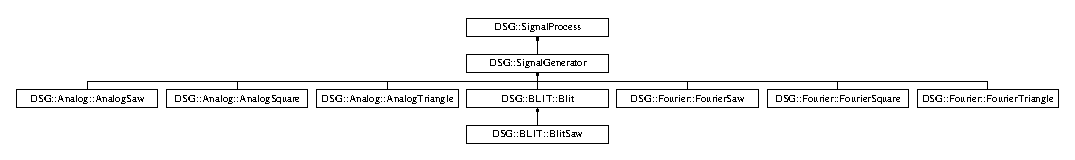
\includegraphics[height=12.000000cm]{class_d_s_g_1_1_signal_generator}
\end{center}
\end{figure}
\subsection*{Public Member Functions}
\begin{DoxyCompactItemize}
\item 
\hyperlink{class_d_s_g_1_1_signal_generator_a13ebda67fcdc880ef41aff501cc23fc3}{Signal\+Generator} ()
\item 
\hyperlink{class_d_s_g_1_1_signal_generator_a4036fceff5c05a3711b8516d850c414c}{Signal\+Generator} (\hyperlink{namespace_d_s_g_a4315a061386fa1014fda09b15d3a6973}{D\+S\+G\+::\+D\+S\+G\+Frequency} const \&frequency, \hyperlink{namespace_d_s_g_a44431ce1eb0a7300efdd207bc879e52c}{D\+S\+G\+::\+D\+S\+G\+Phase} const \&offset)
\item 
virtual \hyperlink{class_d_s_g_1_1_signal_generator_a7b52d391974bc36a19fdcf617ad976cb}{$\sim$\+Signal\+Generator} ()
\item 
virtual bool \hyperlink{class_d_s_g_1_1_signal_generator_a46fe75a81a242e191c5049d33ddf4155}{Perform} (\hyperlink{namespace_d_s_g_ac39a94cd27ebcd9c1e7502d0c624894a}{D\+S\+G\+::\+D\+S\+G\+Sample} \&signal)
\item 
virtual bool \hyperlink{class_d_s_g_1_1_signal_generator_ab050f80e84e6c8b3e354b56930d6a02b}{Perform} (\hyperlink{class_d_s_g_1_1_ring_buffer}{D\+S\+G\+::\+Ring\+Buffer} \&signal)
\item 
virtual \hyperlink{namespace_d_s_g_a4315a061386fa1014fda09b15d3a6973}{D\+S\+G\+::\+D\+S\+G\+Frequency} const \& \hyperlink{class_d_s_g_1_1_signal_generator_a4e6b3c43e76e53f8cd337ad699c464cb}{Frequency} ()
\item 
virtual \hyperlink{namespace_d_s_g_a4315a061386fa1014fda09b15d3a6973}{D\+S\+G\+::\+D\+S\+G\+Frequency} const \& \hyperlink{class_d_s_g_1_1_signal_generator_a30a79888f209d692df3d38f53fc58dfe}{Frequency} (\hyperlink{namespace_d_s_g_a4315a061386fa1014fda09b15d3a6973}{D\+S\+G\+::\+D\+S\+G\+Frequency} const \&value)
\item 
virtual \hyperlink{namespace_d_s_g_a44431ce1eb0a7300efdd207bc879e52c}{D\+S\+G\+::\+D\+S\+G\+Phase} const \& \hyperlink{class_d_s_g_1_1_signal_generator_a17cc4287b2838c6b6194fd43d02e7c00}{Phase} ()
\item 
virtual \hyperlink{namespace_d_s_g_a44431ce1eb0a7300efdd207bc879e52c}{D\+S\+G\+::\+D\+S\+G\+Phase} const \& \hyperlink{class_d_s_g_1_1_signal_generator_a315a3d3fca83eab7030af77dba63a564}{Phase} (\hyperlink{namespace_d_s_g_a44431ce1eb0a7300efdd207bc879e52c}{D\+S\+G\+::\+D\+S\+G\+Phase} const \&value)
\end{DoxyCompactItemize}
\subsection*{Protected Member Functions}
\begin{DoxyCompactItemize}
\item 
void \hyperlink{class_d_s_g_1_1_signal_generator_a4c034c5b9ef3dc7548839288355643d5}{step} ()
\item 
void \hyperlink{class_d_s_g_1_1_signal_generator_a7070f6be04dfd70170328e908b759cd3}{sync} ()
\end{DoxyCompactItemize}
\subsection*{Protected Attributes}
\begin{DoxyCompactItemize}
\item 
\hyperlink{namespace_d_s_g_a4315a061386fa1014fda09b15d3a6973}{D\+S\+G\+::\+D\+S\+G\+Frequency} \hyperlink{class_d_s_g_1_1_signal_generator_a335e7ef058848eca368be51d8544d143}{\+\_\+frequency}
\item 
\hyperlink{namespace_d_s_g_a44431ce1eb0a7300efdd207bc879e52c}{D\+S\+G\+::\+D\+S\+G\+Phase} \hyperlink{class_d_s_g_1_1_signal_generator_a01c046bb52bbb74afd789fdce7978f65}{\+\_\+dt}
\item 
\hyperlink{namespace_d_s_g_a44431ce1eb0a7300efdd207bc879e52c}{D\+S\+G\+::\+D\+S\+G\+Phase} \hyperlink{class_d_s_g_1_1_signal_generator_a12850f2c05838e2234602bd4fde87732}{\+\_\+offset}
\item 
\hyperlink{namespace_d_s_g_a44431ce1eb0a7300efdd207bc879e52c}{D\+S\+G\+::\+D\+S\+G\+Phase} \hyperlink{class_d_s_g_1_1_signal_generator_a1e23eb94e204b11db75fca030b951065}{\+\_\+phasor}
\item 
\hyperlink{namespace_d_s_g_ac39a94cd27ebcd9c1e7502d0c624894a}{D\+S\+G\+::\+D\+S\+G\+Sample} \hyperlink{class_d_s_g_1_1_signal_generator_a28a9b47a1aa0783029f11a19ba0363f2}{\+\_\+storage}
\end{DoxyCompactItemize}


\subsection{Detailed Description}
\hyperlink{class_d_s_g_1_1_signal_generator}{D\+S\+G\+::\+Signal\+Generator} -\/ Extends D\+S\+G\+::\+Signal Process With Tools For Signal Generation. 

Definition at line \hyperlink{_signal_generator_8h_source_l00033}{33} of file \hyperlink{_signal_generator_8h_source}{Signal\+Generator.\+h}.



\subsection{Constructor \& Destructor Documentation}
\hypertarget{class_d_s_g_1_1_signal_generator_a13ebda67fcdc880ef41aff501cc23fc3}{\index{D\+S\+G\+::\+Signal\+Generator@{D\+S\+G\+::\+Signal\+Generator}!Signal\+Generator@{Signal\+Generator}}
\index{Signal\+Generator@{Signal\+Generator}!D\+S\+G\+::\+Signal\+Generator@{D\+S\+G\+::\+Signal\+Generator}}
\subsubsection[{Signal\+Generator}]{\setlength{\rightskip}{0pt plus 5cm}D\+S\+G\+::\+Signal\+Generator\+::\+Signal\+Generator (
\begin{DoxyParamCaption}
{}
\end{DoxyParamCaption}
)}}\label{class_d_s_g_1_1_signal_generator_a13ebda67fcdc880ef41aff501cc23fc3}


Definition at line \hyperlink{_signal_generator_8cpp_source_l00025}{25} of file \hyperlink{_signal_generator_8cpp_source}{Signal\+Generator.\+cpp}.


\begin{DoxyCode}
00025 :\hyperlink{class_d_s_g_1_1_signal_process}{DSG::SignalProcess}(),\hyperlink{class_d_s_g_1_1_signal_generator_a1e23eb94e204b11db75fca030b951065}{\_phasor}(0),\hyperlink{class_d_s_g_1_1_signal_generator_a335e7ef058848eca368be51d8544d143}{\_frequency}(0),
      \hyperlink{class_d_s_g_1_1_signal_generator_a01c046bb52bbb74afd789fdce7978f65}{\_dt}(0),\hyperlink{class_d_s_g_1_1_signal_generator_a12850f2c05838e2234602bd4fde87732}{\_offset}(0)\{\}
\end{DoxyCode}
\hypertarget{class_d_s_g_1_1_signal_generator_a4036fceff5c05a3711b8516d850c414c}{\index{D\+S\+G\+::\+Signal\+Generator@{D\+S\+G\+::\+Signal\+Generator}!Signal\+Generator@{Signal\+Generator}}
\index{Signal\+Generator@{Signal\+Generator}!D\+S\+G\+::\+Signal\+Generator@{D\+S\+G\+::\+Signal\+Generator}}
\subsubsection[{Signal\+Generator}]{\setlength{\rightskip}{0pt plus 5cm}D\+S\+G\+::\+Signal\+Generator\+::\+Signal\+Generator (
\begin{DoxyParamCaption}
\item[{{\bf D\+S\+G\+::\+D\+S\+G\+Frequency} const \&}]{frequency, }
\item[{{\bf D\+S\+G\+::\+D\+S\+G\+Phase} const \&}]{offset}
\end{DoxyParamCaption}
)}}\label{class_d_s_g_1_1_signal_generator_a4036fceff5c05a3711b8516d850c414c}


Definition at line \hyperlink{_signal_generator_8cpp_source_l00026}{26} of file \hyperlink{_signal_generator_8cpp_source}{Signal\+Generator.\+cpp}.


\begin{DoxyCode}
00026                                                                                              :
      \hyperlink{class_d_s_g_1_1_signal_generator_a1e23eb94e204b11db75fca030b951065}{\_phasor}(0),\hyperlink{class_d_s_g_1_1_signal_generator_a335e7ef058848eca368be51d8544d143}{\_frequency}(frequency),\hyperlink{class_d_s_g_1_1_signal_generator_a01c046bb52bbb74afd789fdce7978f65}{\_dt}(0),\hyperlink{class_d_s_g_1_1_signal_generator_a12850f2c05838e2234602bd4fde87732}{\_offset}(offset)\{
00027     \hyperlink{class_d_s_g_1_1_signal_generator_a4e6b3c43e76e53f8cd337ad699c464cb}{Frequency}(frequency);
00028     \hyperlink{class_d_s_g_1_1_signal_generator_a17cc4287b2838c6b6194fd43d02e7c00}{Phase}(offset);
00029 \}
\end{DoxyCode}
\hypertarget{class_d_s_g_1_1_signal_generator_a7b52d391974bc36a19fdcf617ad976cb}{\index{D\+S\+G\+::\+Signal\+Generator@{D\+S\+G\+::\+Signal\+Generator}!````~Signal\+Generator@{$\sim$\+Signal\+Generator}}
\index{````~Signal\+Generator@{$\sim$\+Signal\+Generator}!D\+S\+G\+::\+Signal\+Generator@{D\+S\+G\+::\+Signal\+Generator}}
\subsubsection[{$\sim$\+Signal\+Generator}]{\setlength{\rightskip}{0pt plus 5cm}D\+S\+G\+::\+Signal\+Generator\+::$\sim$\+Signal\+Generator (
\begin{DoxyParamCaption}
{}
\end{DoxyParamCaption}
)\hspace{0.3cm}{\ttfamily [virtual]}}}\label{class_d_s_g_1_1_signal_generator_a7b52d391974bc36a19fdcf617ad976cb}


Definition at line \hyperlink{_signal_generator_8cpp_source_l00030}{30} of file \hyperlink{_signal_generator_8cpp_source}{Signal\+Generator.\+cpp}.


\begin{DoxyCode}
00030 \{\}\end{DoxyCode}


\subsection{Member Function Documentation}
\hypertarget{class_d_s_g_1_1_signal_generator_a4e6b3c43e76e53f8cd337ad699c464cb}{\index{D\+S\+G\+::\+Signal\+Generator@{D\+S\+G\+::\+Signal\+Generator}!Frequency@{Frequency}}
\index{Frequency@{Frequency}!D\+S\+G\+::\+Signal\+Generator@{D\+S\+G\+::\+Signal\+Generator}}
\subsubsection[{Frequency}]{\setlength{\rightskip}{0pt plus 5cm}{\bf D\+S\+G\+::\+D\+S\+G\+Frequency} const \& D\+S\+G\+::\+Signal\+Generator\+::\+Frequency (
\begin{DoxyParamCaption}
{}
\end{DoxyParamCaption}
)\hspace{0.3cm}{\ttfamily [inline]}, {\ttfamily [virtual]}}}\label{class_d_s_g_1_1_signal_generator_a4e6b3c43e76e53f8cd337ad699c464cb}


Definition at line \hyperlink{_signal_generator_8h_source_l00070}{70} of file \hyperlink{_signal_generator_8h_source}{Signal\+Generator.\+h}.


\begin{DoxyCode}
00070                                                            \{
00071     \textcolor{keywordflow}{return} \hyperlink{class_d_s_g_1_1_signal_generator_a335e7ef058848eca368be51d8544d143}{\_frequency};
00072 \}
\end{DoxyCode}
\hypertarget{class_d_s_g_1_1_signal_generator_a30a79888f209d692df3d38f53fc58dfe}{\index{D\+S\+G\+::\+Signal\+Generator@{D\+S\+G\+::\+Signal\+Generator}!Frequency@{Frequency}}
\index{Frequency@{Frequency}!D\+S\+G\+::\+Signal\+Generator@{D\+S\+G\+::\+Signal\+Generator}}
\subsubsection[{Frequency}]{\setlength{\rightskip}{0pt plus 5cm}{\bf D\+S\+G\+::\+D\+S\+G\+Frequency} const \& D\+S\+G\+::\+Signal\+Generator\+::\+Frequency (
\begin{DoxyParamCaption}
\item[{{\bf D\+S\+G\+::\+D\+S\+G\+Frequency} const \&}]{value}
\end{DoxyParamCaption}
)\hspace{0.3cm}{\ttfamily [inline]}, {\ttfamily [virtual]}}}\label{class_d_s_g_1_1_signal_generator_a30a79888f209d692df3d38f53fc58dfe}


Reimplemented in \hyperlink{class_d_s_g_1_1_b_l_i_t_1_1_blit_a933f8f9f324a4fde4f9e2b69473d88ed}{D\+S\+G\+::\+B\+L\+I\+T\+::\+Blit}, \hyperlink{class_d_s_g_1_1_b_l_i_t_1_1_blit_saw_a290d01796efca84b73eb61a3bc419ebb}{D\+S\+G\+::\+B\+L\+I\+T\+::\+Blit\+Saw}, \hyperlink{class_d_s_g_1_1_fourier_1_1_fourier_saw_afa3d86f404be3665f10c74fe9286ef10}{D\+S\+G\+::\+Fourier\+::\+Fourier\+Saw}, \hyperlink{class_d_s_g_1_1_fourier_1_1_fourier_square_a120cbb563a518c9412190eaa36cb269f}{D\+S\+G\+::\+Fourier\+::\+Fourier\+Square}, and \hyperlink{class_d_s_g_1_1_fourier_1_1_fourier_triangle_a278a51ed8af32ea371adc903b9b25039}{D\+S\+G\+::\+Fourier\+::\+Fourier\+Triangle}.



Definition at line \hyperlink{_signal_generator_8h_source_l00073}{73} of file \hyperlink{_signal_generator_8h_source}{Signal\+Generator.\+h}.


\begin{DoxyCode}
00073                                                                                        \{
00074     \hyperlink{class_d_s_g_1_1_signal_generator_a335e7ef058848eca368be51d8544d143}{\_frequency} = DSG::EnforceBounds<0, 20000,DSG::DSGSample>(value);
00075     \hyperlink{class_d_s_g_1_1_signal_generator_a01c046bb52bbb74afd789fdce7978f65}{\_dt} = \hyperlink{class_d_s_g_1_1_signal_generator_a335e7ef058848eca368be51d8544d143}{\_frequency}/\hyperlink{namespace_d_s_g_a72df05177db0412c3590070923f62819}{DSG::SampleRate}();
00076     \textcolor{keywordflow}{return} \hyperlink{class_d_s_g_1_1_signal_generator_a335e7ef058848eca368be51d8544d143}{\_frequency};
00077 \}
\end{DoxyCode}
\hypertarget{class_d_s_g_1_1_signal_generator_a46fe75a81a242e191c5049d33ddf4155}{\index{D\+S\+G\+::\+Signal\+Generator@{D\+S\+G\+::\+Signal\+Generator}!Perform@{Perform}}
\index{Perform@{Perform}!D\+S\+G\+::\+Signal\+Generator@{D\+S\+G\+::\+Signal\+Generator}}
\subsubsection[{Perform}]{\setlength{\rightskip}{0pt plus 5cm}bool D\+S\+G\+::\+Signal\+Generator\+::\+Perform (
\begin{DoxyParamCaption}
\item[{{\bf D\+S\+G\+::\+D\+S\+G\+Sample} \&}]{signal}
\end{DoxyParamCaption}
)\hspace{0.3cm}{\ttfamily [inline]}, {\ttfamily [virtual]}}}\label{class_d_s_g_1_1_signal_generator_a46fe75a81a242e191c5049d33ddf4155}


Implements \hyperlink{class_d_s_g_1_1_signal_process_af73d246c460915db7a9be7e3ef36844d}{D\+S\+G\+::\+Signal\+Process}.



Reimplemented in \hyperlink{class_d_s_g_1_1_fourier_1_1_fourier_series_generator_aa4768d44397b5fab5a30cb86068e161a}{D\+S\+G\+::\+Fourier\+::\+Fourier\+Series\+Generator}, \hyperlink{class_d_s_g_1_1_b_l_i_t_1_1_blit_adfd7c8891b4c4dbd0530a2780781b2bd}{D\+S\+G\+::\+B\+L\+I\+T\+::\+Blit}, \hyperlink{class_d_s_g_1_1_d_p_w_1_1_d_p_w_saw_a8d0bffad58e9bce19fe737302de749ed}{D\+S\+G\+::\+D\+P\+W\+::\+D\+P\+W\+Saw$<$ order $>$}, \hyperlink{class_d_s_g_1_1_e_p_t_r_1_1_e_p_t_r_saw_aa253efa41cca56f334ccb0fd32c2cd56}{D\+S\+G\+::\+E\+P\+T\+R\+::\+E\+P\+T\+R\+Saw}, \hyperlink{class_d_s_g_1_1_analog_1_1_analog_saw_a8d36e77c09ba84128e786c7bb14cddda}{D\+S\+G\+::\+Analog\+::\+Analog\+Saw}, \hyperlink{class_d_s_g_1_1_analog_1_1_analog_square_a784aa17d266704647789b972cf880e9f}{D\+S\+G\+::\+Analog\+::\+Analog\+Square}, \hyperlink{class_d_s_g_1_1_analog_1_1_analog_triangle_a9b2484f3eb4c4ad545cb88b8833be124}{D\+S\+G\+::\+Analog\+::\+Analog\+Triangle}, \hyperlink{class_d_s_g_1_1_b_l_i_t_1_1_blit_saw_ae24821c51b23b9fe9220a620e558af04}{D\+S\+G\+::\+B\+L\+I\+T\+::\+Blit\+Saw}, \hyperlink{class_d_s_g_1_1_fourier_1_1_fourier_saw_a33061612ff24180f12e9a2c29dfaa116}{D\+S\+G\+::\+Fourier\+::\+Fourier\+Saw}, \hyperlink{class_d_s_g_1_1_fourier_1_1_fourier_square_a05bd0cd3e76ca22e1cede5afb47fbbc4}{D\+S\+G\+::\+Fourier\+::\+Fourier\+Square}, \hyperlink{class_d_s_g_1_1_fourier_1_1_fourier_triangle_ab5b947c1fc1f34a461c863b18e3e877d}{D\+S\+G\+::\+Fourier\+::\+Fourier\+Triangle}, and \hyperlink{class_d_s_g_1_1_generic_generator_addcd9abbbf0e31f0af2ff18217a08302}{D\+S\+G\+::\+Generic\+Generator}.



Definition at line \hyperlink{_signal_generator_8h_source_l00062}{62} of file \hyperlink{_signal_generator_8h_source}{Signal\+Generator.\+h}.


\begin{DoxyCode}
00062                                                            \{
00063     signal=0;
00064     \textcolor{keywordflow}{return} \textcolor{keyword}{false};
00065 \}
\end{DoxyCode}
\hypertarget{class_d_s_g_1_1_signal_generator_ab050f80e84e6c8b3e354b56930d6a02b}{\index{D\+S\+G\+::\+Signal\+Generator@{D\+S\+G\+::\+Signal\+Generator}!Perform@{Perform}}
\index{Perform@{Perform}!D\+S\+G\+::\+Signal\+Generator@{D\+S\+G\+::\+Signal\+Generator}}
\subsubsection[{Perform}]{\setlength{\rightskip}{0pt plus 5cm}bool D\+S\+G\+::\+Signal\+Generator\+::\+Perform (
\begin{DoxyParamCaption}
\item[{{\bf D\+S\+G\+::\+Ring\+Buffer} \&}]{signal}
\end{DoxyParamCaption}
)\hspace{0.3cm}{\ttfamily [inline]}, {\ttfamily [virtual]}}}\label{class_d_s_g_1_1_signal_generator_ab050f80e84e6c8b3e354b56930d6a02b}


Implements \hyperlink{class_d_s_g_1_1_signal_process_a2c8ff3487d9c43f9eace1d9192d4a37e}{D\+S\+G\+::\+Signal\+Process}.



Reimplemented in \hyperlink{class_d_s_g_1_1_d_p_w_1_1_d_p_w_saw_a03548019c5ec057f5980a4bd99a0d3f0}{D\+S\+G\+::\+D\+P\+W\+::\+D\+P\+W\+Saw$<$ order $>$}, \hyperlink{class_d_s_g_1_1_fourier_1_1_fourier_series_generator_adce79a239104570f8a6565e708fb70a7}{D\+S\+G\+::\+Fourier\+::\+Fourier\+Series\+Generator}, \hyperlink{class_d_s_g_1_1_b_l_i_t_1_1_blit_aab7c67ff8f059c8367ba316cf8cd5436}{D\+S\+G\+::\+B\+L\+I\+T\+::\+Blit}, \hyperlink{class_d_s_g_1_1_e_p_t_r_1_1_e_p_t_r_saw_a9dbefaeeb74e30e722bb5d8ea767cdca}{D\+S\+G\+::\+E\+P\+T\+R\+::\+E\+P\+T\+R\+Saw}, \hyperlink{class_d_s_g_1_1_analog_1_1_analog_saw_a38f091059d924c9141fee3e27522e7e1}{D\+S\+G\+::\+Analog\+::\+Analog\+Saw}, \hyperlink{class_d_s_g_1_1_analog_1_1_analog_square_af4d41d5894ae02e920c61e06cf041c60}{D\+S\+G\+::\+Analog\+::\+Analog\+Square}, \hyperlink{class_d_s_g_1_1_analog_1_1_analog_triangle_a568c994e0f83f6a01d813357259a8f37}{D\+S\+G\+::\+Analog\+::\+Analog\+Triangle}, \hyperlink{class_d_s_g_1_1_b_l_i_t_1_1_blit_saw_ad2edba8ed83558e76afed6ec1d5cf4d6}{D\+S\+G\+::\+B\+L\+I\+T\+::\+Blit\+Saw}, \hyperlink{class_d_s_g_1_1_fourier_1_1_fourier_saw_ac890d9f0af523b63b96b07e6696a32b7}{D\+S\+G\+::\+Fourier\+::\+Fourier\+Saw}, \hyperlink{class_d_s_g_1_1_fourier_1_1_fourier_square_a46028a3615f26876f9c613f983141362}{D\+S\+G\+::\+Fourier\+::\+Fourier\+Square}, \hyperlink{class_d_s_g_1_1_fourier_1_1_fourier_triangle_a27b082e69cc7d70223dd3fbc552ba5bc}{D\+S\+G\+::\+Fourier\+::\+Fourier\+Triangle}, and \hyperlink{class_d_s_g_1_1_generic_generator_a886544537d2f77243ec42dad9f124a8d}{D\+S\+G\+::\+Generic\+Generator}.



Definition at line \hyperlink{_signal_generator_8h_source_l00066}{66} of file \hyperlink{_signal_generator_8h_source}{Signal\+Generator.\+h}.


\begin{DoxyCode}
00066                                                             \{
00067     signal.\hyperlink{class_d_s_g_1_1_ring_buffer_ab23c8003d2857809a816068eeb209d60}{Flush}();
00068     \textcolor{keywordflow}{return} \textcolor{keyword}{false};
00069 \}
\end{DoxyCode}
\hypertarget{class_d_s_g_1_1_signal_generator_a17cc4287b2838c6b6194fd43d02e7c00}{\index{D\+S\+G\+::\+Signal\+Generator@{D\+S\+G\+::\+Signal\+Generator}!Phase@{Phase}}
\index{Phase@{Phase}!D\+S\+G\+::\+Signal\+Generator@{D\+S\+G\+::\+Signal\+Generator}}
\subsubsection[{Phase}]{\setlength{\rightskip}{0pt plus 5cm}{\bf D\+S\+G\+::\+D\+S\+G\+Phase} const \& D\+S\+G\+::\+Signal\+Generator\+::\+Phase (
\begin{DoxyParamCaption}
{}
\end{DoxyParamCaption}
)\hspace{0.3cm}{\ttfamily [inline]}, {\ttfamily [virtual]}}}\label{class_d_s_g_1_1_signal_generator_a17cc4287b2838c6b6194fd43d02e7c00}


Definition at line \hyperlink{_signal_generator_8h_source_l00078}{78} of file \hyperlink{_signal_generator_8h_source}{Signal\+Generator.\+h}.


\begin{DoxyCode}
00078                                                    \{
00079     \textcolor{keywordflow}{return} \hyperlink{class_d_s_g_1_1_signal_generator_a12850f2c05838e2234602bd4fde87732}{\_offset};
00080 \}
\end{DoxyCode}
\hypertarget{class_d_s_g_1_1_signal_generator_a315a3d3fca83eab7030af77dba63a564}{\index{D\+S\+G\+::\+Signal\+Generator@{D\+S\+G\+::\+Signal\+Generator}!Phase@{Phase}}
\index{Phase@{Phase}!D\+S\+G\+::\+Signal\+Generator@{D\+S\+G\+::\+Signal\+Generator}}
\subsubsection[{Phase}]{\setlength{\rightskip}{0pt plus 5cm}{\bf D\+S\+G\+::\+D\+S\+G\+Phase} const \& D\+S\+G\+::\+Signal\+Generator\+::\+Phase (
\begin{DoxyParamCaption}
\item[{{\bf D\+S\+G\+::\+D\+S\+G\+Phase} const \&}]{value}
\end{DoxyParamCaption}
)\hspace{0.3cm}{\ttfamily [inline]}, {\ttfamily [virtual]}}}\label{class_d_s_g_1_1_signal_generator_a315a3d3fca83eab7030af77dba63a564}


Definition at line \hyperlink{_signal_generator_8h_source_l00081}{81} of file \hyperlink{_signal_generator_8h_source}{Signal\+Generator.\+h}.


\begin{DoxyCode}
00081                                                                            \{
00082     \hyperlink{class_d_s_g_1_1_signal_generator_a12850f2c05838e2234602bd4fde87732}{\_offset}-=value;
00083     \hyperlink{class_d_s_g_1_1_signal_generator_a1e23eb94e204b11db75fca030b951065}{\_phasor}-=\hyperlink{class_d_s_g_1_1_signal_generator_a12850f2c05838e2234602bd4fde87732}{\_offset};
00084     \hyperlink{class_d_s_g_1_1_signal_generator_a12850f2c05838e2234602bd4fde87732}{\_offset}=value;
00085     \textcolor{keywordflow}{return} \hyperlink{class_d_s_g_1_1_signal_generator_a12850f2c05838e2234602bd4fde87732}{\_offset};
00086 \}
\end{DoxyCode}
\hypertarget{class_d_s_g_1_1_signal_generator_a4c034c5b9ef3dc7548839288355643d5}{\index{D\+S\+G\+::\+Signal\+Generator@{D\+S\+G\+::\+Signal\+Generator}!step@{step}}
\index{step@{step}!D\+S\+G\+::\+Signal\+Generator@{D\+S\+G\+::\+Signal\+Generator}}
\subsubsection[{step}]{\setlength{\rightskip}{0pt plus 5cm}void D\+S\+G\+::\+Signal\+Generator\+::step (
\begin{DoxyParamCaption}
{}
\end{DoxyParamCaption}
)\hspace{0.3cm}{\ttfamily [inline]}, {\ttfamily [protected]}}}\label{class_d_s_g_1_1_signal_generator_a4c034c5b9ef3dc7548839288355643d5}


Definition at line \hyperlink{_signal_generator_8h_source_l00087}{87} of file \hyperlink{_signal_generator_8h_source}{Signal\+Generator.\+h}.


\begin{DoxyCode}
00087                                     \{
00088     \hyperlink{class_d_s_g_1_1_signal_generator_a1e23eb94e204b11db75fca030b951065}{\_phasor}+=\hyperlink{class_d_s_g_1_1_signal_generator_a01c046bb52bbb74afd789fdce7978f65}{\_dt};
00089     \hyperlink{class_d_s_g_1_1_signal_generator_a1e23eb94e204b11db75fca030b951065}{\_phasor}>1.0 ? --\hyperlink{class_d_s_g_1_1_signal_generator_a1e23eb94e204b11db75fca030b951065}{\_phasor}:0;
00090 \}
\end{DoxyCode}
\hypertarget{class_d_s_g_1_1_signal_generator_a7070f6be04dfd70170328e908b759cd3}{\index{D\+S\+G\+::\+Signal\+Generator@{D\+S\+G\+::\+Signal\+Generator}!sync@{sync}}
\index{sync@{sync}!D\+S\+G\+::\+Signal\+Generator@{D\+S\+G\+::\+Signal\+Generator}}
\subsubsection[{sync}]{\setlength{\rightskip}{0pt plus 5cm}void D\+S\+G\+::\+Signal\+Generator\+::sync (
\begin{DoxyParamCaption}
{}
\end{DoxyParamCaption}
)\hspace{0.3cm}{\ttfamily [inline]}, {\ttfamily [protected]}}}\label{class_d_s_g_1_1_signal_generator_a7070f6be04dfd70170328e908b759cd3}


Definition at line \hyperlink{_signal_generator_8h_source_l00091}{91} of file \hyperlink{_signal_generator_8h_source}{Signal\+Generator.\+h}.


\begin{DoxyCode}
00091                                     \{
00092     \hyperlink{class_d_s_g_1_1_signal_generator_a1e23eb94e204b11db75fca030b951065}{\_phasor}=\hyperlink{class_d_s_g_1_1_signal_generator_a12850f2c05838e2234602bd4fde87732}{\_offset};
00093 \}
\end{DoxyCode}


\subsection{Member Data Documentation}
\hypertarget{class_d_s_g_1_1_signal_generator_a01c046bb52bbb74afd789fdce7978f65}{\index{D\+S\+G\+::\+Signal\+Generator@{D\+S\+G\+::\+Signal\+Generator}!\+\_\+dt@{\+\_\+dt}}
\index{\+\_\+dt@{\+\_\+dt}!D\+S\+G\+::\+Signal\+Generator@{D\+S\+G\+::\+Signal\+Generator}}
\subsubsection[{\+\_\+dt}]{\setlength{\rightskip}{0pt plus 5cm}{\bf D\+S\+G\+::\+D\+S\+G\+Phase} D\+S\+G\+::\+Signal\+Generator\+::\+\_\+dt\hspace{0.3cm}{\ttfamily [protected]}}}\label{class_d_s_g_1_1_signal_generator_a01c046bb52bbb74afd789fdce7978f65}


Definition at line \hyperlink{_signal_generator_8h_source_l00051}{51} of file \hyperlink{_signal_generator_8h_source}{Signal\+Generator.\+h}.

\hypertarget{class_d_s_g_1_1_signal_generator_a335e7ef058848eca368be51d8544d143}{\index{D\+S\+G\+::\+Signal\+Generator@{D\+S\+G\+::\+Signal\+Generator}!\+\_\+frequency@{\+\_\+frequency}}
\index{\+\_\+frequency@{\+\_\+frequency}!D\+S\+G\+::\+Signal\+Generator@{D\+S\+G\+::\+Signal\+Generator}}
\subsubsection[{\+\_\+frequency}]{\setlength{\rightskip}{0pt plus 5cm}{\bf D\+S\+G\+::\+D\+S\+G\+Frequency} D\+S\+G\+::\+Signal\+Generator\+::\+\_\+frequency\hspace{0.3cm}{\ttfamily [protected]}}}\label{class_d_s_g_1_1_signal_generator_a335e7ef058848eca368be51d8544d143}


Definition at line \hyperlink{_signal_generator_8h_source_l00050}{50} of file \hyperlink{_signal_generator_8h_source}{Signal\+Generator.\+h}.

\hypertarget{class_d_s_g_1_1_signal_generator_a12850f2c05838e2234602bd4fde87732}{\index{D\+S\+G\+::\+Signal\+Generator@{D\+S\+G\+::\+Signal\+Generator}!\+\_\+offset@{\+\_\+offset}}
\index{\+\_\+offset@{\+\_\+offset}!D\+S\+G\+::\+Signal\+Generator@{D\+S\+G\+::\+Signal\+Generator}}
\subsubsection[{\+\_\+offset}]{\setlength{\rightskip}{0pt plus 5cm}{\bf D\+S\+G\+::\+D\+S\+G\+Phase} D\+S\+G\+::\+Signal\+Generator\+::\+\_\+offset\hspace{0.3cm}{\ttfamily [protected]}}}\label{class_d_s_g_1_1_signal_generator_a12850f2c05838e2234602bd4fde87732}


Definition at line \hyperlink{_signal_generator_8h_source_l00052}{52} of file \hyperlink{_signal_generator_8h_source}{Signal\+Generator.\+h}.

\hypertarget{class_d_s_g_1_1_signal_generator_a1e23eb94e204b11db75fca030b951065}{\index{D\+S\+G\+::\+Signal\+Generator@{D\+S\+G\+::\+Signal\+Generator}!\+\_\+phasor@{\+\_\+phasor}}
\index{\+\_\+phasor@{\+\_\+phasor}!D\+S\+G\+::\+Signal\+Generator@{D\+S\+G\+::\+Signal\+Generator}}
\subsubsection[{\+\_\+phasor}]{\setlength{\rightskip}{0pt plus 5cm}{\bf D\+S\+G\+::\+D\+S\+G\+Phase} D\+S\+G\+::\+Signal\+Generator\+::\+\_\+phasor\hspace{0.3cm}{\ttfamily [protected]}}}\label{class_d_s_g_1_1_signal_generator_a1e23eb94e204b11db75fca030b951065}


Definition at line \hyperlink{_signal_generator_8h_source_l00053}{53} of file \hyperlink{_signal_generator_8h_source}{Signal\+Generator.\+h}.

\hypertarget{class_d_s_g_1_1_signal_generator_a28a9b47a1aa0783029f11a19ba0363f2}{\index{D\+S\+G\+::\+Signal\+Generator@{D\+S\+G\+::\+Signal\+Generator}!\+\_\+storage@{\+\_\+storage}}
\index{\+\_\+storage@{\+\_\+storage}!D\+S\+G\+::\+Signal\+Generator@{D\+S\+G\+::\+Signal\+Generator}}
\subsubsection[{\+\_\+storage}]{\setlength{\rightskip}{0pt plus 5cm}{\bf D\+S\+G\+::\+D\+S\+G\+Sample} D\+S\+G\+::\+Signal\+Generator\+::\+\_\+storage\hspace{0.3cm}{\ttfamily [protected]}}}\label{class_d_s_g_1_1_signal_generator_a28a9b47a1aa0783029f11a19ba0363f2}


Definition at line \hyperlink{_signal_generator_8h_source_l00054}{54} of file \hyperlink{_signal_generator_8h_source}{Signal\+Generator.\+h}.



The documentation for this class was generated from the following files\+:\begin{DoxyCompactItemize}
\item 
\hyperlink{_signal_generator_8h}{Signal\+Generator.\+h}\item 
\hyperlink{_signal_generator_8cpp}{Signal\+Generator.\+cpp}\end{DoxyCompactItemize}

\hypertarget{class_d_s_g_1_1_signal_process}{\section{D\+S\+G\+:\+:Signal\+Process Class Reference}
\label{class_d_s_g_1_1_signal_process}\index{D\+S\+G\+::\+Signal\+Process@{D\+S\+G\+::\+Signal\+Process}}
}


\hyperlink{class_d_s_g_1_1_signal_process}{D\+S\+G\+::\+Signal\+Process} -\/ Defines Base Interface For Audio Processing.  




{\ttfamily \#include $<$Signal\+Process.\+h$>$}

Inheritance diagram for D\+S\+G\+:\+:Signal\+Process\+:\begin{figure}[H]
\begin{center}
\leavevmode
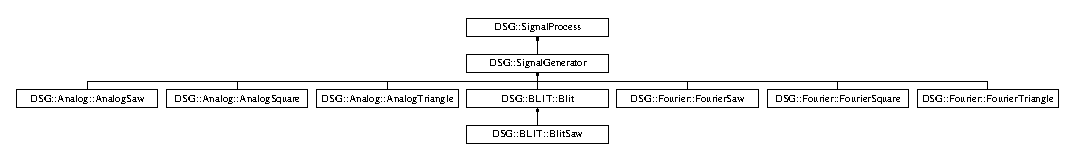
\includegraphics[height=1.702128cm]{class_d_s_g_1_1_signal_process}
\end{center}
\end{figure}
\subsection*{Public Member Functions}
\begin{DoxyCompactItemize}
\item 
\hypertarget{class_d_s_g_1_1_signal_process_af73d246c460915db7a9be7e3ef36844d}{virtual bool {\bfseries Perform} (D\+S\+G\+::\+D\+S\+G\+Sample \&signal)=0}\label{class_d_s_g_1_1_signal_process_af73d246c460915db7a9be7e3ef36844d}

\item 
\hypertarget{class_d_s_g_1_1_signal_process_a2c8ff3487d9c43f9eace1d9192d4a37e}{virtual bool {\bfseries Perform} (\hyperlink{class_d_s_g_1_1_ring_buffer}{D\+S\+G\+::\+Ring\+Buffer} \&signal)=0}\label{class_d_s_g_1_1_signal_process_a2c8ff3487d9c43f9eace1d9192d4a37e}

\end{DoxyCompactItemize}


\subsection{Detailed Description}
\hyperlink{class_d_s_g_1_1_signal_process}{D\+S\+G\+::\+Signal\+Process} -\/ Defines Base Interface For Audio Processing. 

The documentation for this class was generated from the following files\+:\begin{DoxyCompactItemize}
\item 
/\+Users/alexanderzywicki/\+Documents/\+D\+S\+G/src/Signal\+Process.\+h\item 
/\+Users/alexanderzywicki/\+Documents/\+D\+S\+G/src/Signal\+Process.\+cpp\end{DoxyCompactItemize}

\hypertarget{class_d_s_g_1_1_sine_l_u_t}{\section{D\+S\+G\+:\+:Sine\+L\+U\+T$<$ element, size $>$ Class Template Reference}
\label{class_d_s_g_1_1_sine_l_u_t}\index{D\+S\+G\+::\+Sine\+L\+U\+T$<$ element, size $>$@{D\+S\+G\+::\+Sine\+L\+U\+T$<$ element, size $>$}}
}
Inheritance diagram for D\+S\+G\+:\+:Sine\+L\+U\+T$<$ element, size $>$\+:\begin{figure}[H]
\begin{center}
\leavevmode
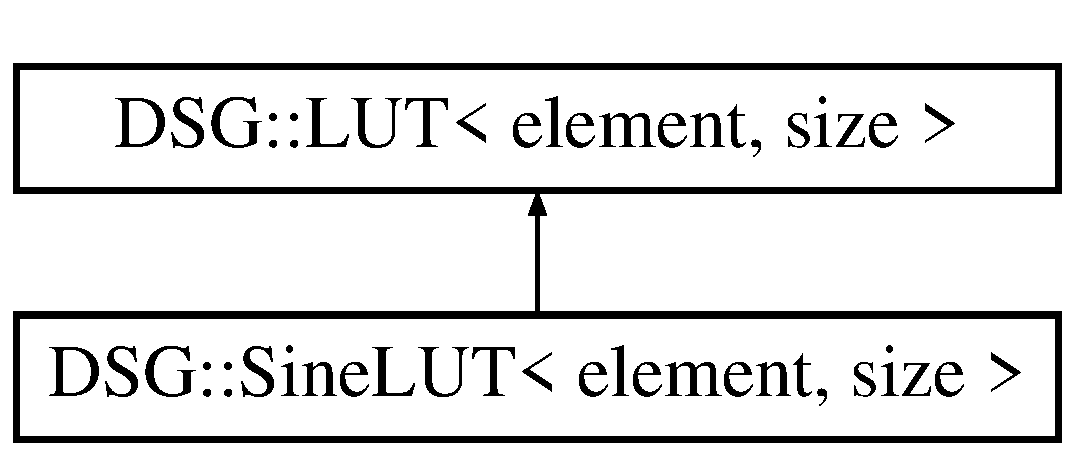
\includegraphics[height=2.000000cm]{class_d_s_g_1_1_sine_l_u_t}
\end{center}
\end{figure}
\subsection*{Public Member Functions}
\begin{DoxyCompactItemize}
\item 
\hypertarget{class_d_s_g_1_1_sine_l_u_t_a1373f5663138855be2ea01999b6d6ac8}{virtual element const \& {\bfseries operator()} (double const \&x)}\label{class_d_s_g_1_1_sine_l_u_t_a1373f5663138855be2ea01999b6d6ac8}

\end{DoxyCompactItemize}
\subsection*{Protected Attributes}
\begin{DoxyCompactItemize}
\item 
\hypertarget{class_d_s_g_1_1_sine_l_u_t_ae780e53f58e2c7dc0568ee96f2d5598b}{double {\bfseries phs}}\label{class_d_s_g_1_1_sine_l_u_t_ae780e53f58e2c7dc0568ee96f2d5598b}

\end{DoxyCompactItemize}


The documentation for this class was generated from the following file\+:\begin{DoxyCompactItemize}
\item 
/\+Users/alexanderzywicki/\+Documents/\+D\+S\+G/src/Sine\+L\+U\+T.\+h\end{DoxyCompactItemize}

\hypertarget{class_d_s_g_1_1_small_sine_l_u_t}{\section{D\+S\+G\+:\+:Small\+Sine\+L\+U\+T$<$ element, size $>$ Class Template Reference}
\label{class_d_s_g_1_1_small_sine_l_u_t}\index{D\+S\+G\+::\+Small\+Sine\+L\+U\+T$<$ element, size $>$@{D\+S\+G\+::\+Small\+Sine\+L\+U\+T$<$ element, size $>$}}
}
Inheritance diagram for D\+S\+G\+:\+:Small\+Sine\+L\+U\+T$<$ element, size $>$\+:\begin{figure}[H]
\begin{center}
\leavevmode
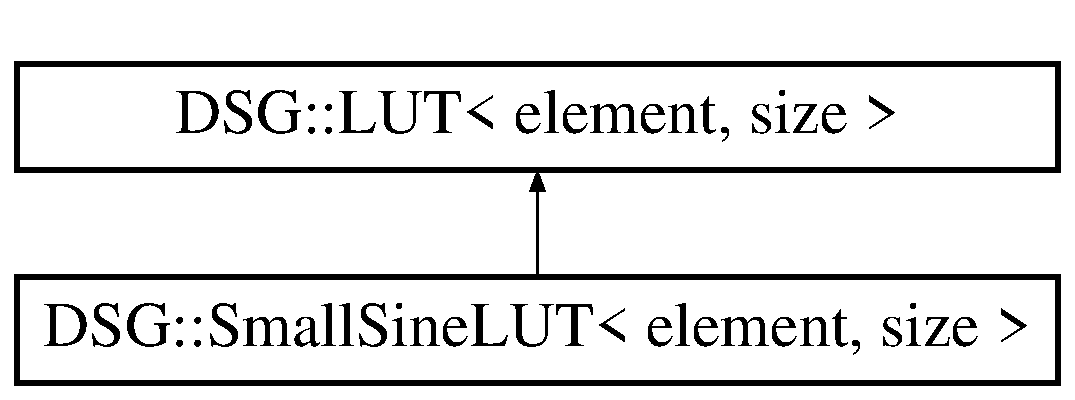
\includegraphics[height=2.000000cm]{class_d_s_g_1_1_small_sine_l_u_t}
\end{center}
\end{figure}
\subsection*{Public Member Functions}
\begin{DoxyCompactItemize}
\item 
\hypertarget{class_d_s_g_1_1_small_sine_l_u_t_a411742ddafa9551ea099f644dd88e75e}{virtual element {\bfseries operator()} (double const \&x)}\label{class_d_s_g_1_1_small_sine_l_u_t_a411742ddafa9551ea099f644dd88e75e}

\end{DoxyCompactItemize}
\subsection*{Protected Member Functions}
\begin{DoxyCompactItemize}
\item 
\hypertarget{class_d_s_g_1_1_small_sine_l_u_t_a3c0e550d2bc8b96ab430a4c290254d70}{void {\bfseries fill} ()}\label{class_d_s_g_1_1_small_sine_l_u_t_a3c0e550d2bc8b96ab430a4c290254d70}

\item 
\hypertarget{class_d_s_g_1_1_small_sine_l_u_t_a2835eea620f319931b60af632b696d9d}{element const \& {\bfseries lookup} (double index)}\label{class_d_s_g_1_1_small_sine_l_u_t_a2835eea620f319931b60af632b696d9d}

\end{DoxyCompactItemize}
\subsection*{Additional Inherited Members}


The documentation for this class was generated from the following file\+:\begin{DoxyCompactItemize}
\item 
/\+Users/alexanderzywicki/\+Documents/\+D\+S\+G/src/Sine\+L\+U\+T.\+h\end{DoxyCompactItemize}

\hypertarget{class_d_s_g_1_1_small_sine_l_u_t_3_01int32__t_00_01size_01_4}{\section{D\+S\+G\+:\+:Small\+Sine\+L\+U\+T$<$ int32\+\_\+t, size $>$ Class Template Reference}
\label{class_d_s_g_1_1_small_sine_l_u_t_3_01int32__t_00_01size_01_4}\index{D\+S\+G\+::\+Small\+Sine\+L\+U\+T$<$ int32\+\_\+t, size $>$@{D\+S\+G\+::\+Small\+Sine\+L\+U\+T$<$ int32\+\_\+t, size $>$}}
}
Inheritance diagram for D\+S\+G\+:\+:Small\+Sine\+L\+U\+T$<$ int32\+\_\+t, size $>$\+:\begin{figure}[H]
\begin{center}
\leavevmode
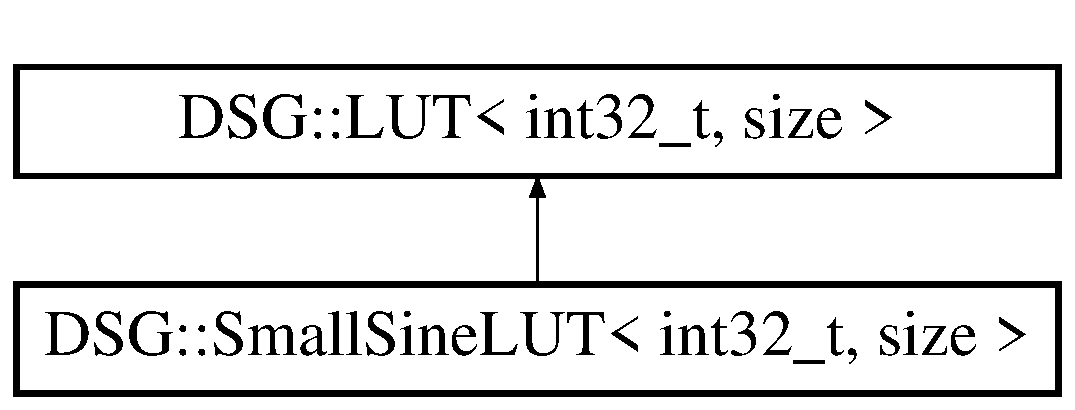
\includegraphics[height=2.000000cm]{class_d_s_g_1_1_small_sine_l_u_t_3_01int32__t_00_01size_01_4}
\end{center}
\end{figure}
\subsection*{Public Member Functions}
\begin{DoxyCompactItemize}
\item 
\hypertarget{class_d_s_g_1_1_small_sine_l_u_t_3_01int32__t_00_01size_01_4_a63873dafa3ddb5c6c36fa2c2c1ab5bf7}{virtual int32\+\_\+t {\bfseries operator()} (double const \&x)}\label{class_d_s_g_1_1_small_sine_l_u_t_3_01int32__t_00_01size_01_4_a63873dafa3ddb5c6c36fa2c2c1ab5bf7}

\end{DoxyCompactItemize}
\subsection*{Protected Member Functions}
\begin{DoxyCompactItemize}
\item 
\hypertarget{class_d_s_g_1_1_small_sine_l_u_t_3_01int32__t_00_01size_01_4_a5f08d4c634a95d05edb6dec411df4270}{void {\bfseries fill} ()}\label{class_d_s_g_1_1_small_sine_l_u_t_3_01int32__t_00_01size_01_4_a5f08d4c634a95d05edb6dec411df4270}

\item 
\hypertarget{class_d_s_g_1_1_small_sine_l_u_t_3_01int32__t_00_01size_01_4_ab2ba369359e94c52febf2dbff7abdc67}{int32\+\_\+t const \& {\bfseries lookup} (double \&\&index)}\label{class_d_s_g_1_1_small_sine_l_u_t_3_01int32__t_00_01size_01_4_ab2ba369359e94c52febf2dbff7abdc67}

\end{DoxyCompactItemize}
\subsection*{Additional Inherited Members}


The documentation for this class was generated from the following file\+:\begin{DoxyCompactItemize}
\item 
/\+Users/alexanderzywicki/\+Documents/\+D\+S\+G/src/Sine\+L\+U\+T.\+h\end{DoxyCompactItemize}

%--- End generated contents ---

% Index
\newpage
\phantomsection
\addcontentsline{toc}{chapter}{Index}
\printindex

\end{document}
